\section{Signal modelling}
\label{sec:signal_model}

The parameterization of \mfl distributions based on simulated samples for signals are described in this section.
Several signal models are studied, including heavy Higgs like narrow-width signal (NWA) and large-width signal (LWA), as well as the modelling of Randall-Sundrum graviton (RSG) signal.

%% ========================================================================================================================
%% NWA

\subsection{Modelling of narrow-width signal}
\label{sec:signal_nwa}

For narrow-width (NWA) signal, the \mfl width is totally determined by detector resolution, which is modelled 
by the sum of a Crystal Ball ($\mathcal{C}$) function~\cite{CrystalBall1,CrystalBall2} and a Gaussian ($\mathcal{G}$) function:

\begin{equation}
    \label{eq:cb_plus_g}
    P_{s} (\mfl) = f_{\mathcal{C}} \cdot \mathcal{C}(\mfl; \mu, \sigma_{\mathcal{C}}, \alpha_{\mathcal{C}}, n_{\mathcal{C}})
                   + (1 - f_{\mathcal{C}}) \cdot \mathcal{G}(\mfl; \mu, \sigma_{\mathcal{G}})
\end{equation}

The two functions share the same central value $\mu$, while the resolution parameters, $\sigma_{\mathcal{C}}$ and $\sigma_{\mathcal{G}}$, are different.
In the Crystal Ball function, the parameters $\alpha_{\mathcal{C}}$ and $n_{\mathcal{C}}$ model the shape of non-Gaussian tail,
and the fraction parameter $f_{\mathcal{C}}$ is used to ensure the relative normalization between two functions.

The parameters are obtained by fitting to signal MC simulations combining the mc16a, mc16d and mc16e campaigns for each category at each mass points from 200~\gev~ to 2000~\gev~ respectively,
and the shape of ggF and VBF signals are found to be similar.
Figure~\ref{fig:ggf_mass_signalParam_2mu2e} shows the \mfl distribution and fitted curves for ggF production at mass from 200~\gev~ to 2000~\gev~ in 2$e$2$\mu$ channel as examples.

\begin{figure}[htbp]
    \centering
    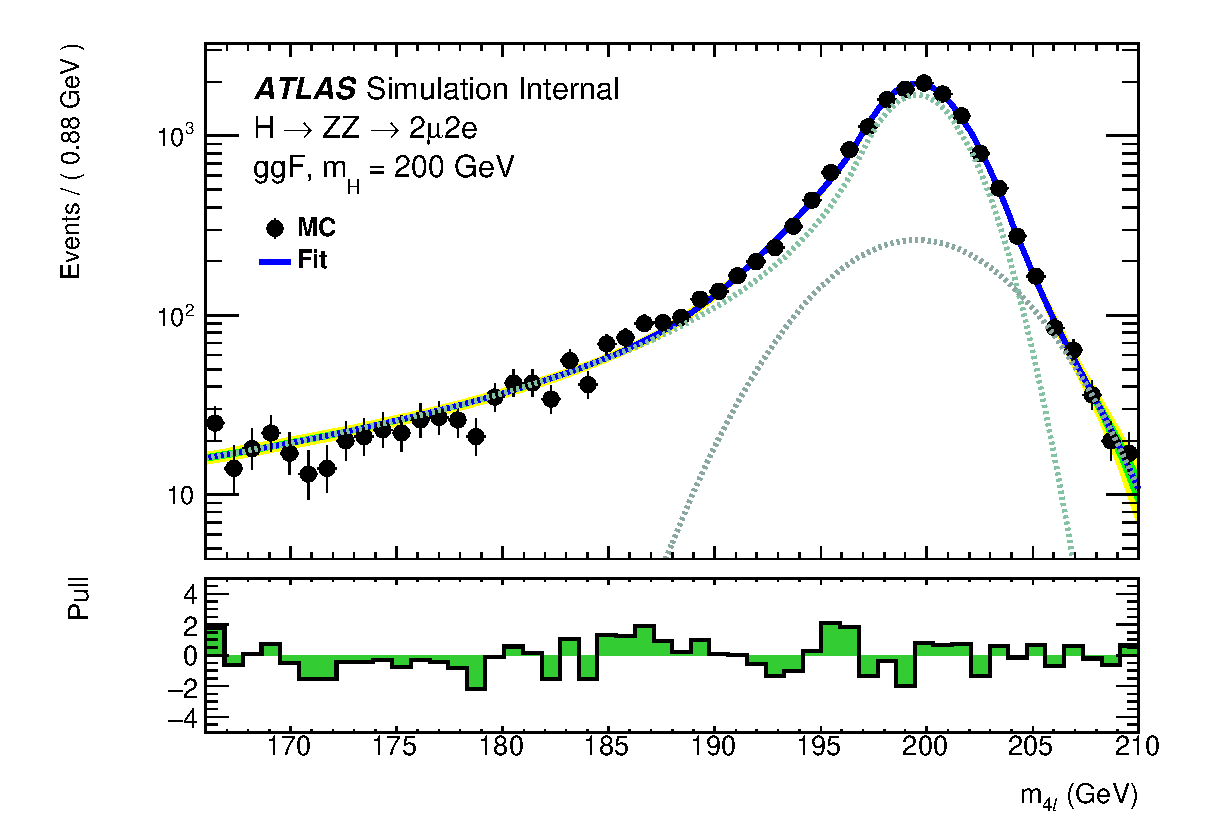
\includegraphics[width=0.32\textwidth]{figures/HMHZZ/signal/NWA//ggf_mass_signal_200_H4l_2mu2e.eps}
    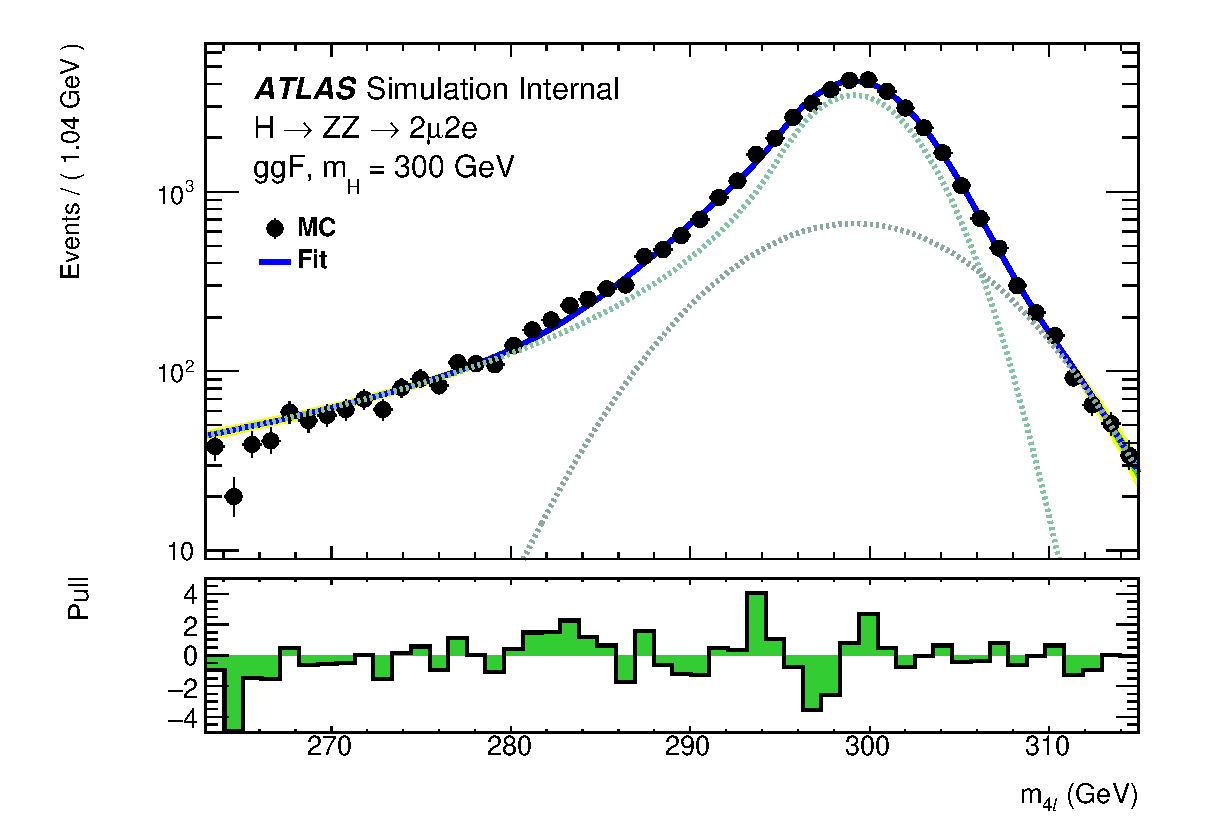
\includegraphics[width=0.32\textwidth]{figures/HMHZZ/signal/NWA//ggf_mass_signal_300_H4l_2mu2e.eps}
    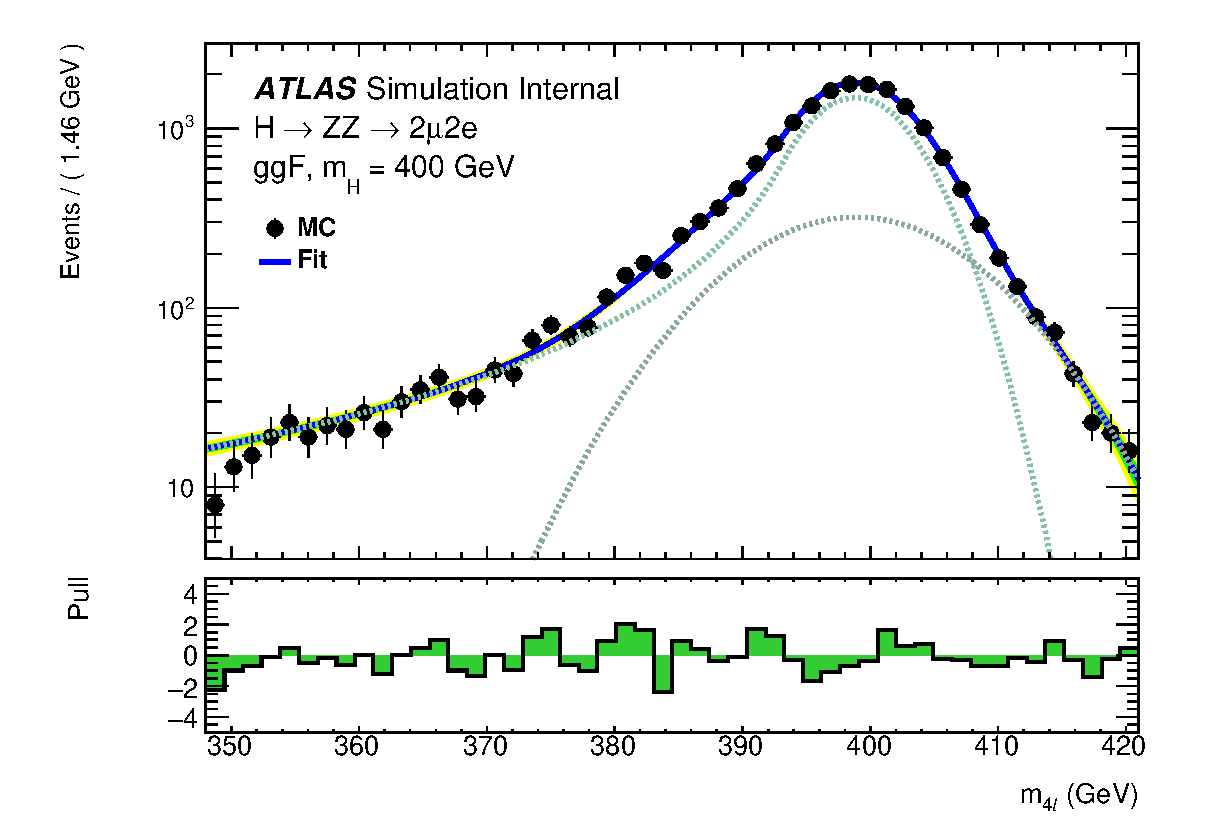
\includegraphics[width=0.32\textwidth]{figures/HMHZZ/signal/NWA//ggf_mass_signal_400_H4l_2mu2e.eps}\\
    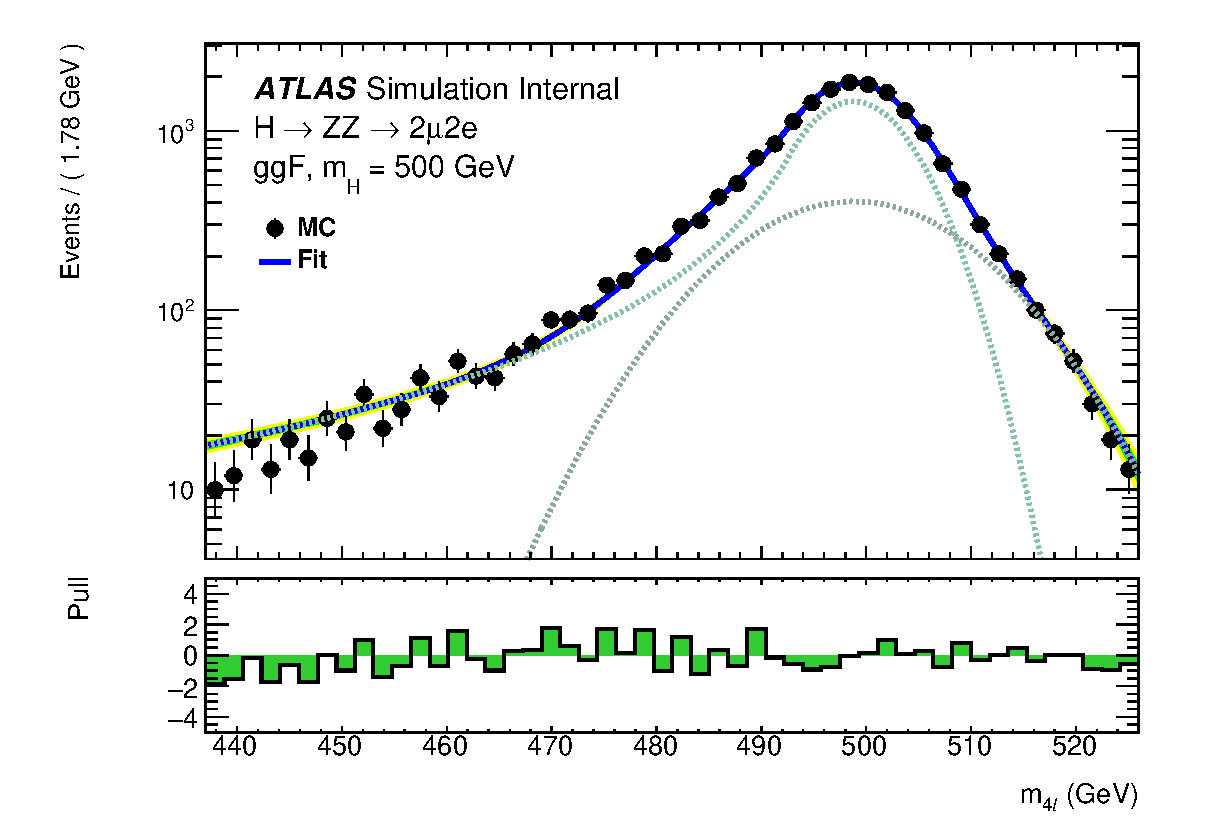
\includegraphics[width=0.32\textwidth]{figures/HMHZZ/signal/NWA//ggf_mass_signal_500_H4l_2mu2e.eps}
    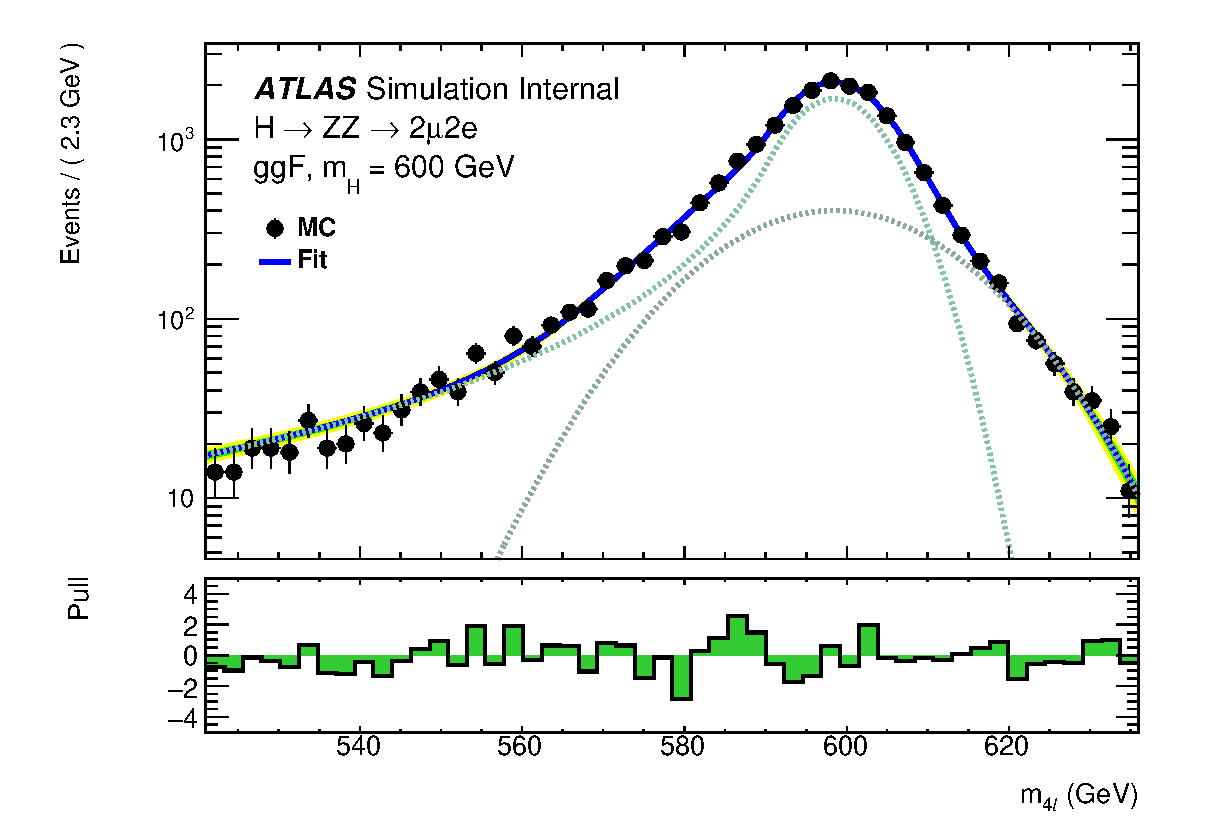
\includegraphics[width=0.32\textwidth]{figures/HMHZZ/signal/NWA//ggf_mass_signal_600_H4l_2mu2e.eps}
    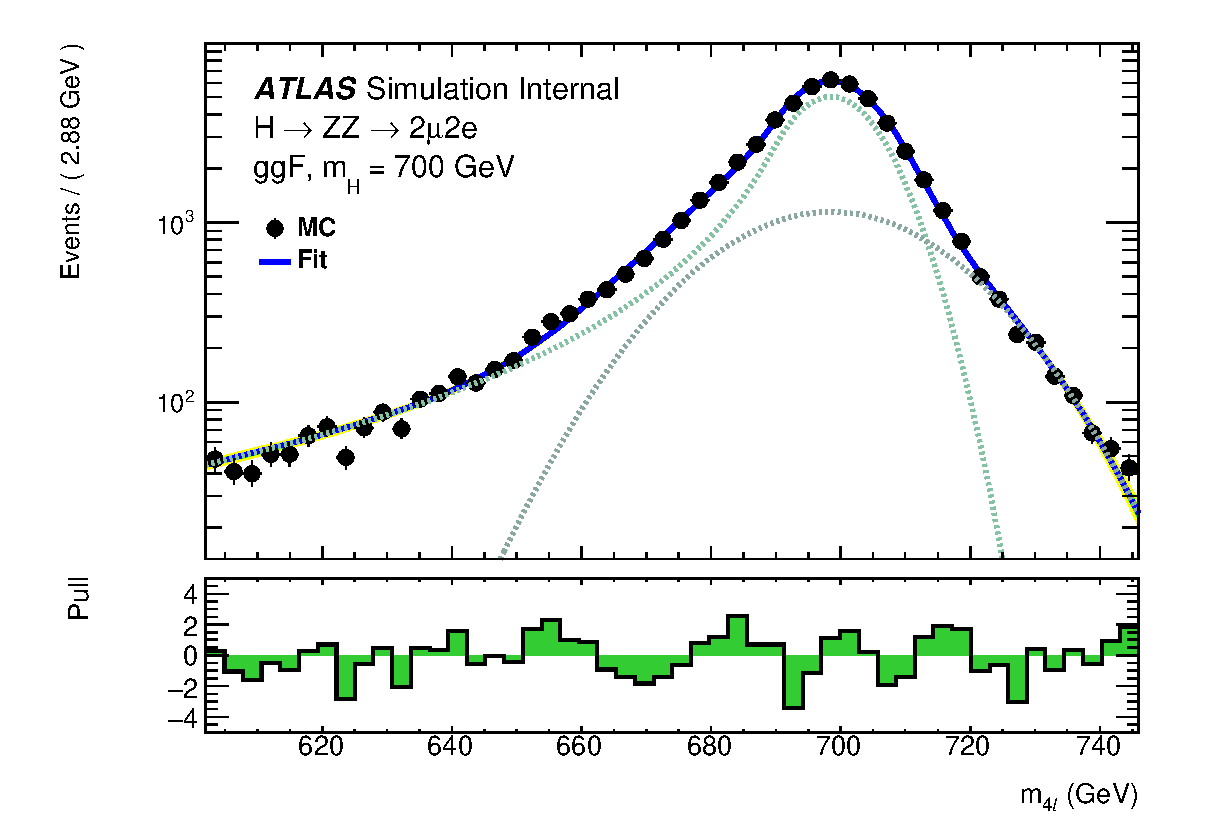
\includegraphics[width=0.32\textwidth]{figures/HMHZZ/signal/NWA//ggf_mass_signal_700_H4l_2mu2e.eps}\\
    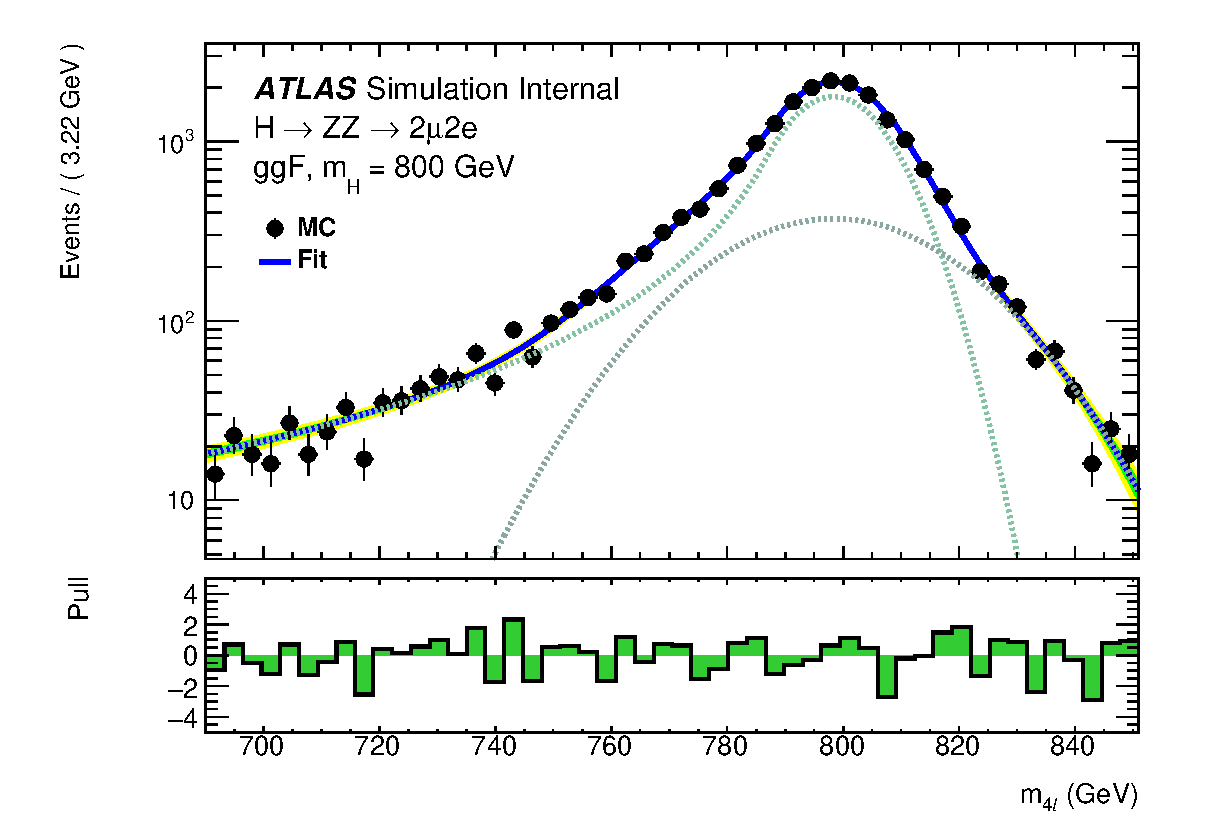
\includegraphics[width=0.32\textwidth]{figures/HMHZZ/signal/NWA//ggf_mass_signal_800_H4l_2mu2e.eps}
    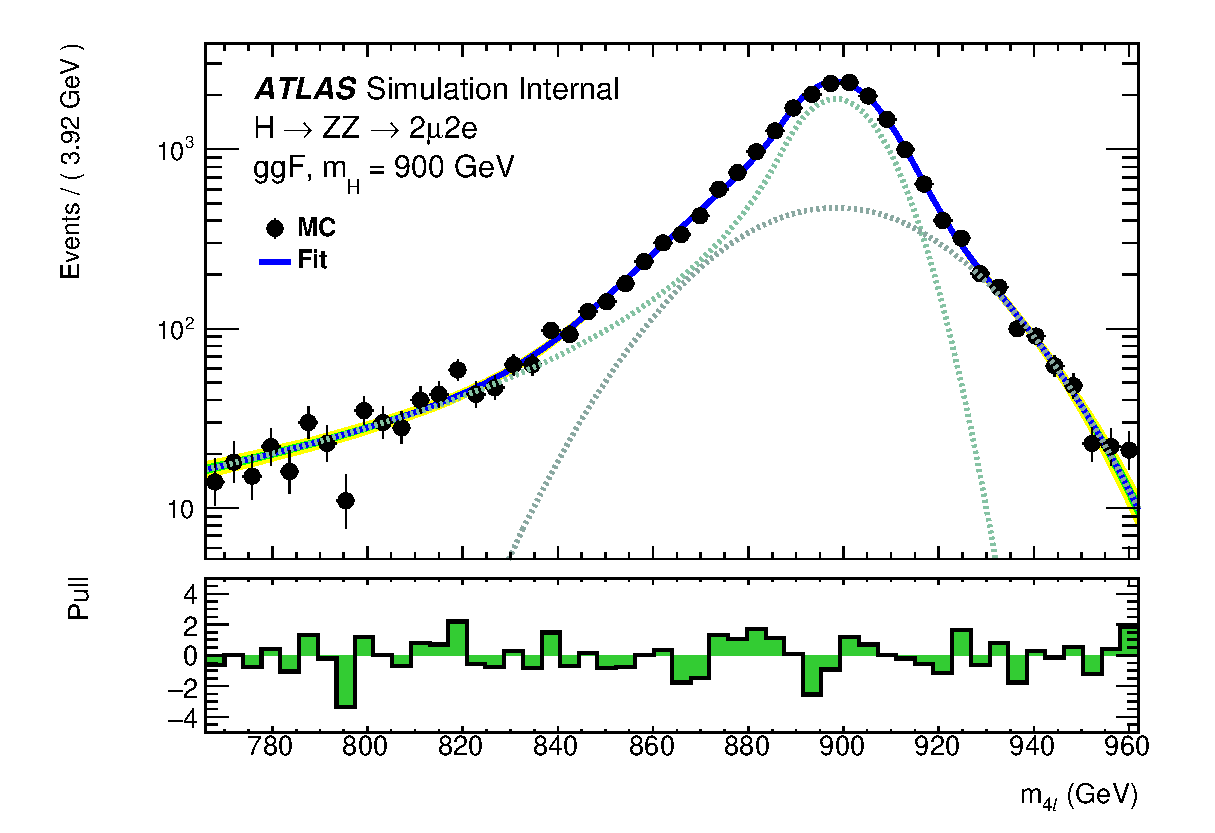
\includegraphics[width=0.32\textwidth]{figures/HMHZZ/signal/NWA//ggf_mass_signal_900_H4l_2mu2e.eps}
    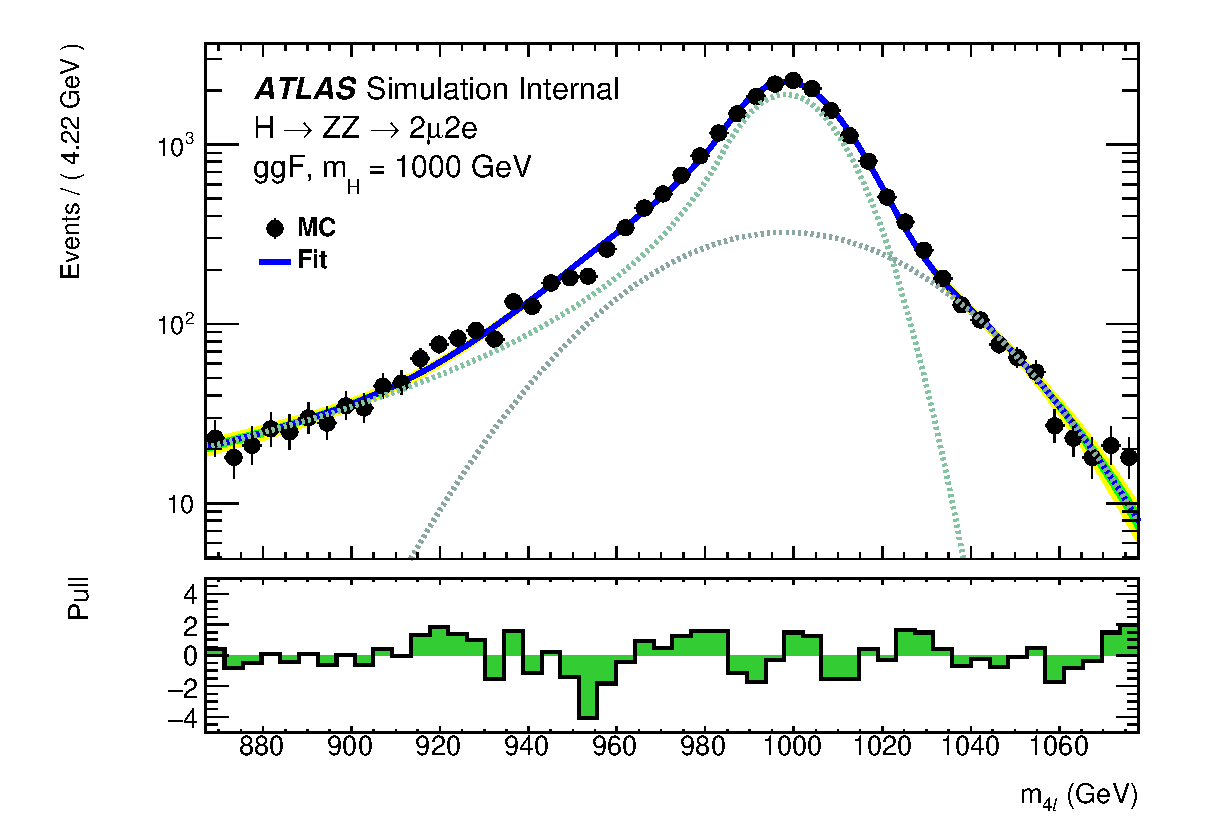
\includegraphics[width=0.32\textwidth]{figures/HMHZZ/signal/NWA//ggf_mass_signal_1000_H4l_2mu2e.eps}\\
    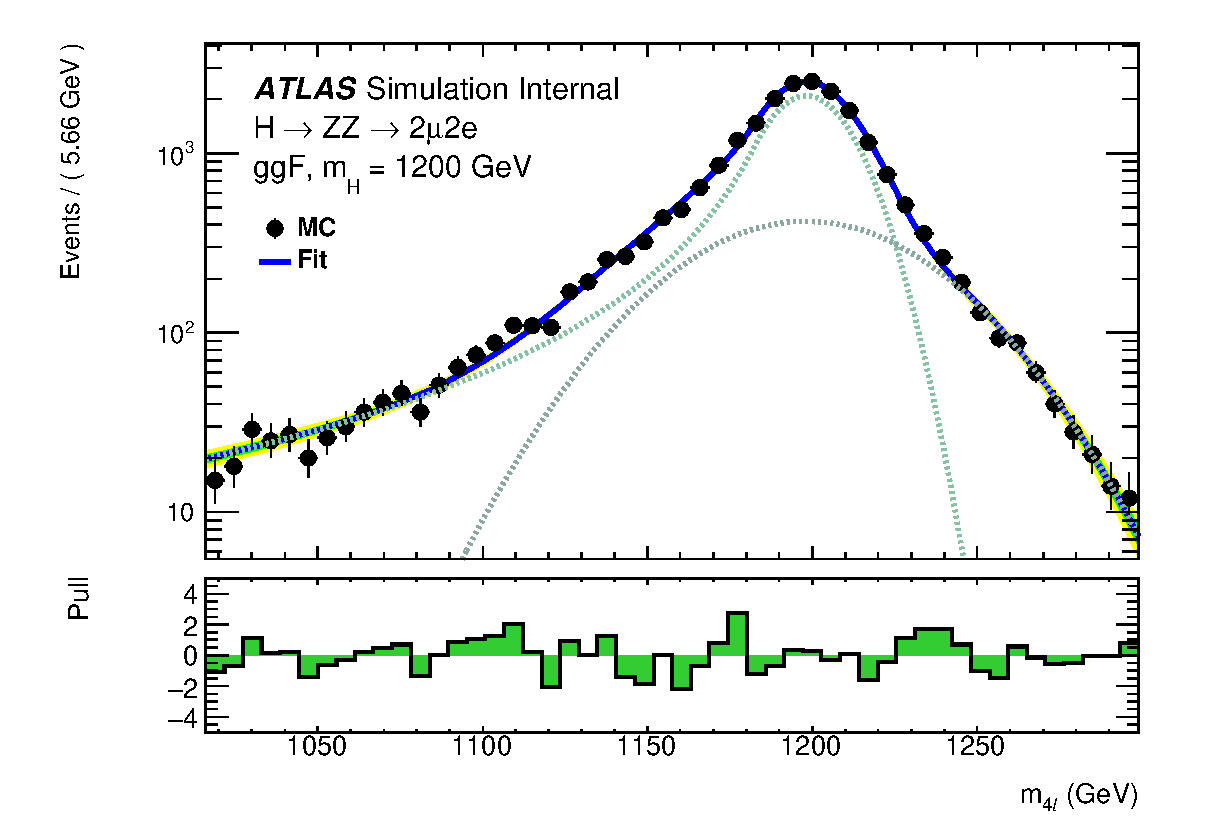
\includegraphics[width=0.32\textwidth]{figures/HMHZZ/signal/NWA//ggf_mass_signal_1200_H4l_2mu2e.eps}
    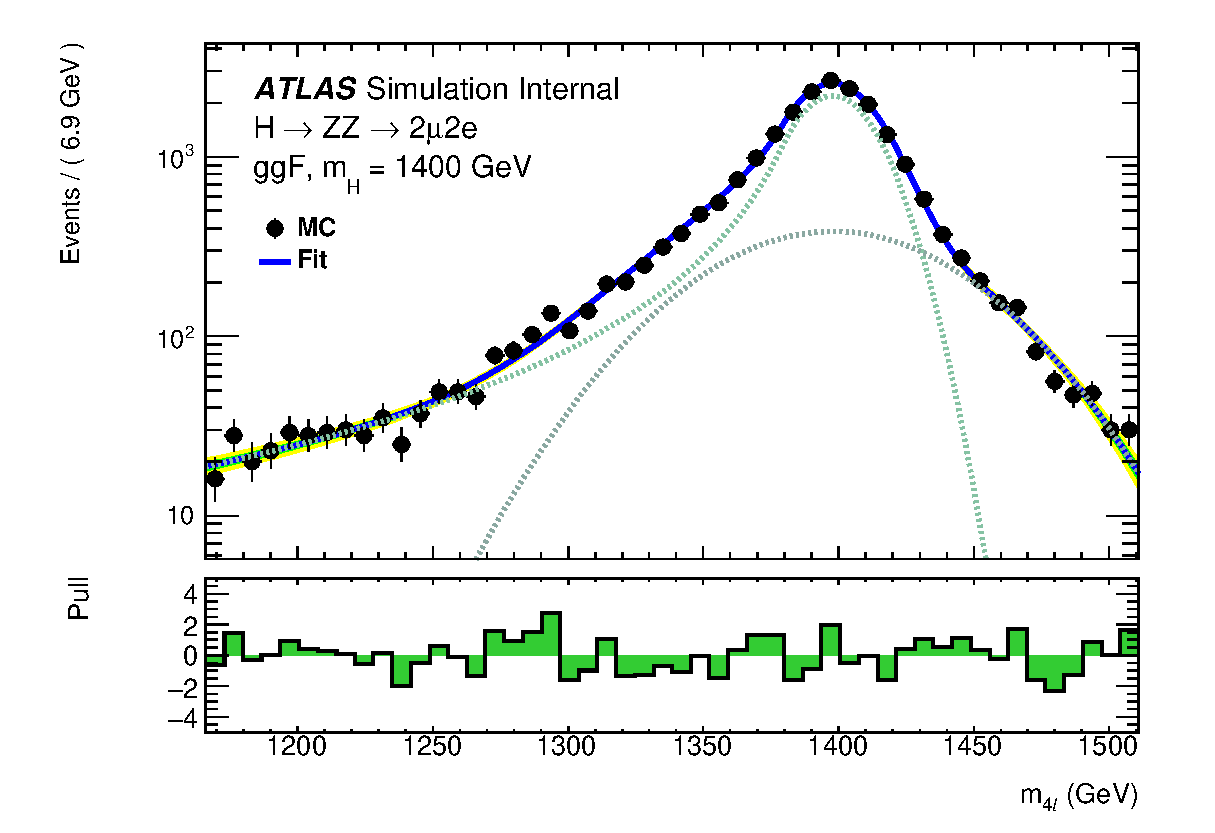
\includegraphics[width=0.32\textwidth]{figures/HMHZZ/signal/NWA//ggf_mass_signal_1400_H4l_2mu2e.eps}
    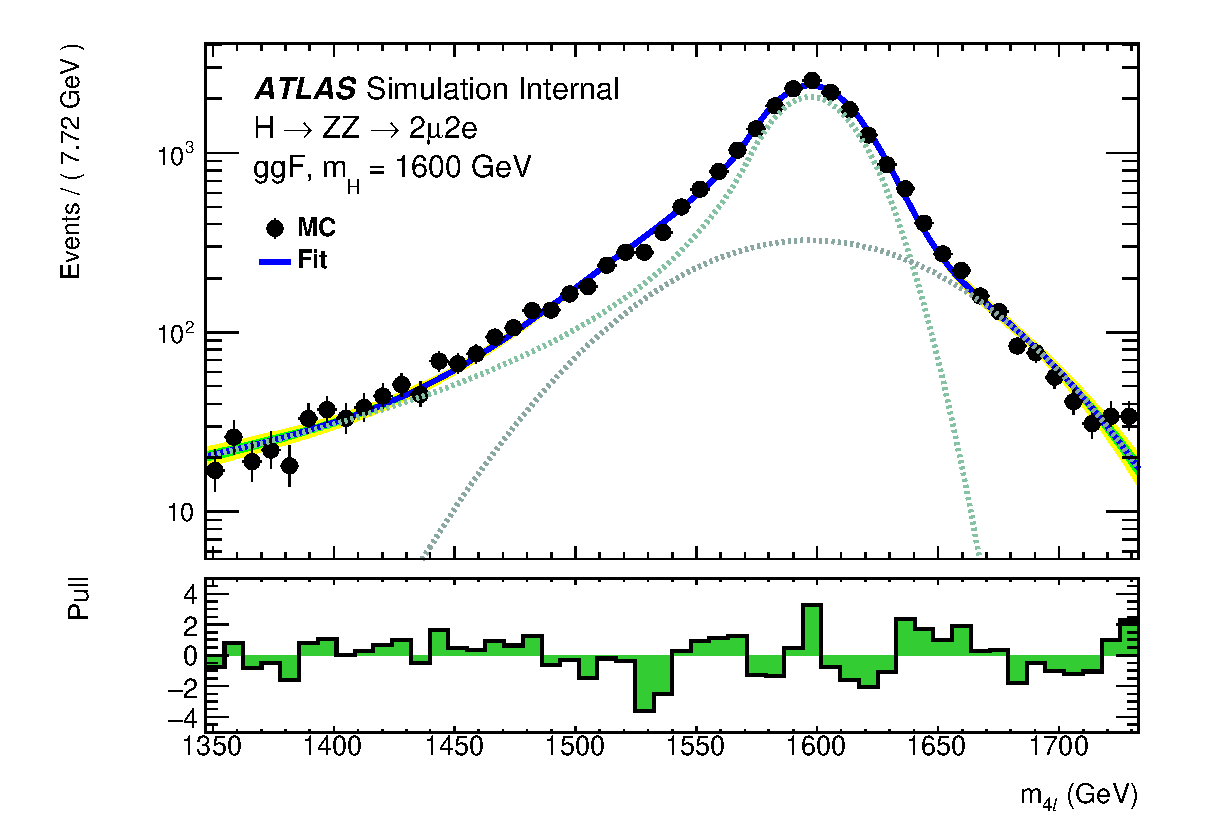
\includegraphics[width=0.32\textwidth]{figures/HMHZZ/signal/NWA//ggf_mass_signal_1600_H4l_2mu2e.eps}\\
    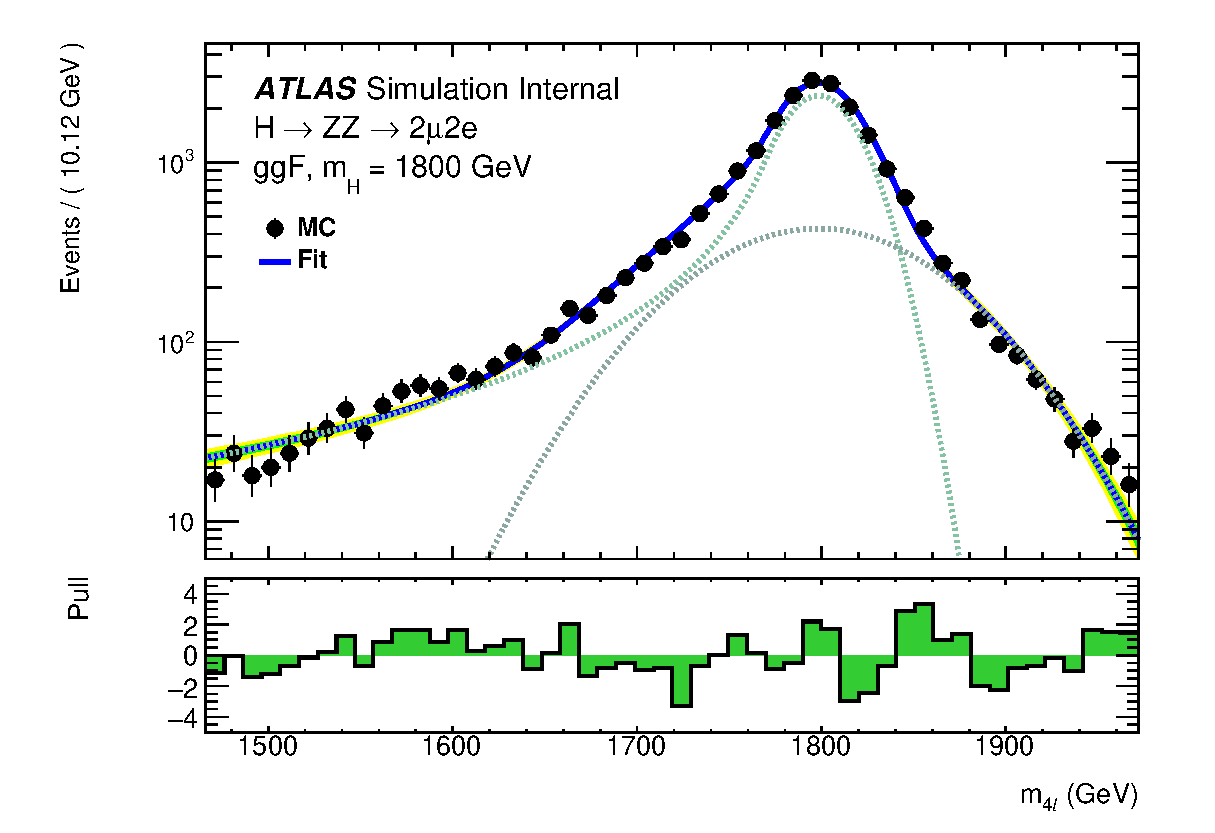
\includegraphics[width=0.32\textwidth]{figures/HMHZZ/signal/NWA//ggf_mass_signal_1800_H4l_2mu2e.eps}
    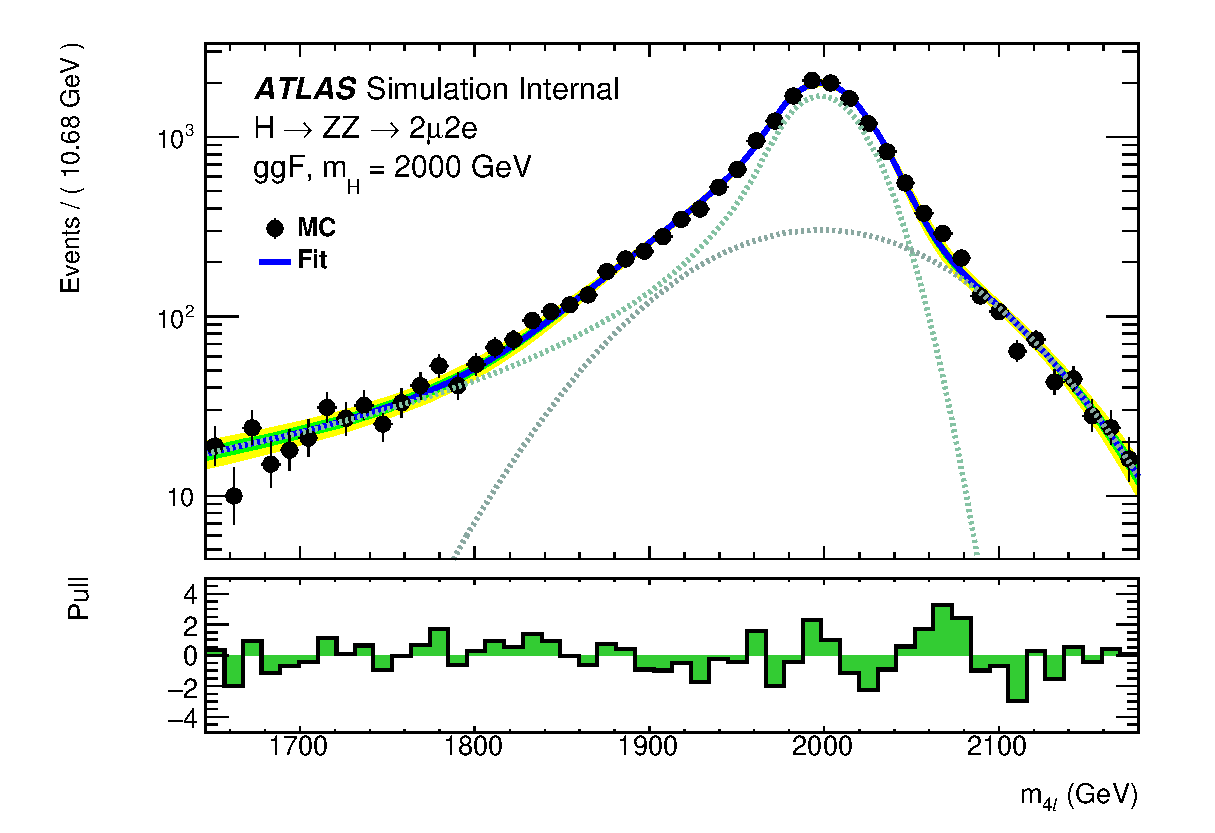
\includegraphics[width=0.32\textwidth]{figures/HMHZZ/signal/NWA//ggf_mass_signal_2000_H4l_2mu2e.eps}
    \caption{Distributions of the $m_{2\mu 2e}$ and fit projection for signal samples between 200 to 3000~\gev for ggF production mode. 
    Three MC campaigns, mc16a, mc16d and mc16e, are combined. 
    The lower panel in each plot shows the pull distribution.}
    \label{fig:ggf_mass_signalParam_2mu2e}
\end{figure}

Then the $\mathcal{C}+\mathcal{G}$ parameters are fitted with a polynomial function as the function of generated mass points (\mH), as an example shown in figure~\ref{fig:ggf_fitParams_interpolation_2mu2e} for ggF production in 2$e$2$\mu$ channel.
The fitting quality can be measured by the Pearson's $\chi^2$, which is within 3 (2) for 2$e$2$\mu$ (4$e$ and 4$\mu$) channel.

\begin{figure}[htbp]
    \centering
    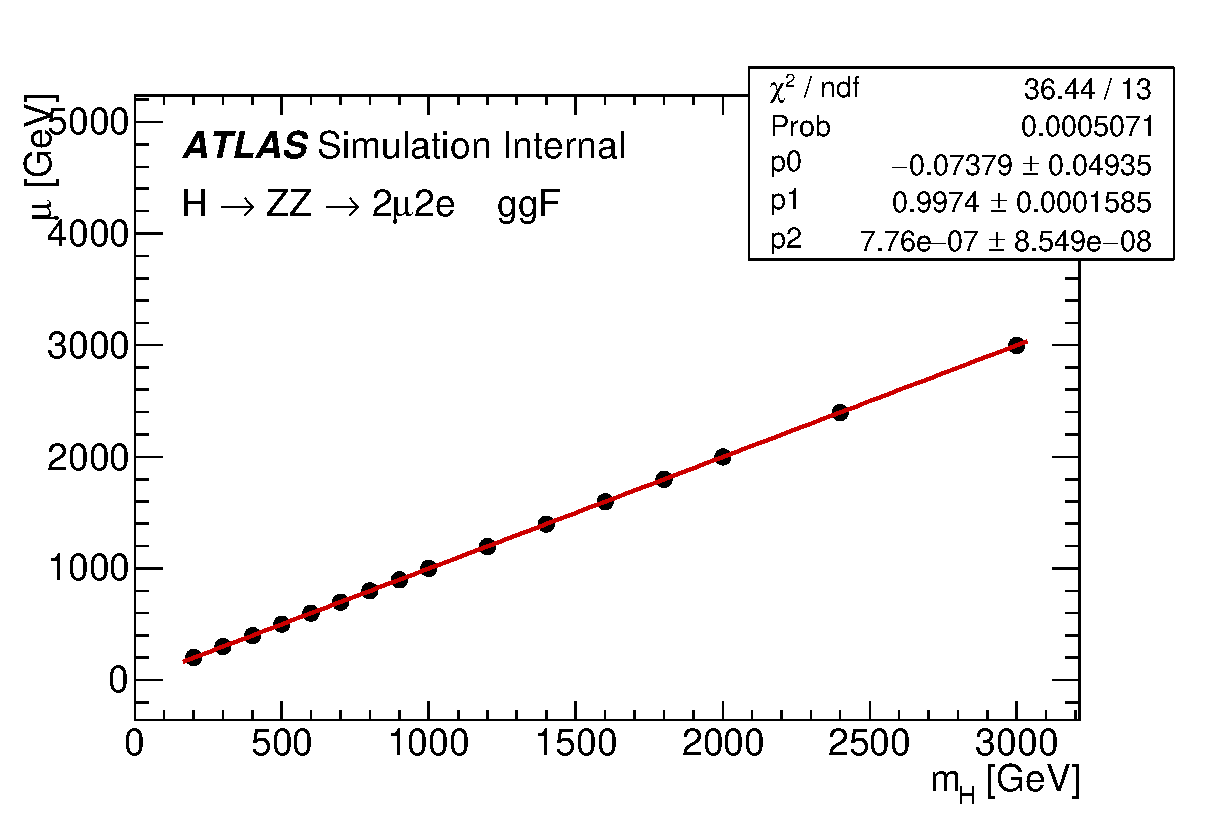
\includegraphics[width=0.32\textwidth]{figures/HMHZZ/signal/NWA//ggf_graph_mass_mean_2mu2e_fit.eps}
    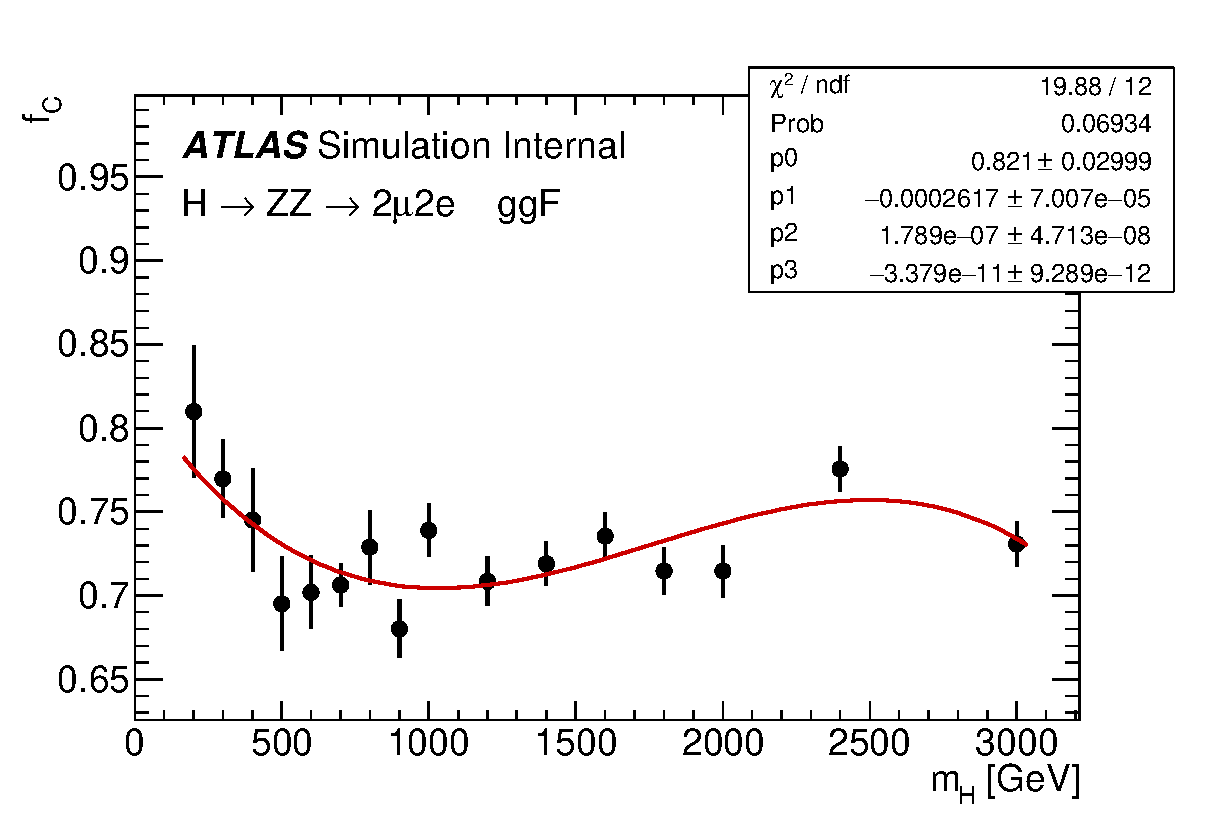
\includegraphics[width=0.32\textwidth]{figures/HMHZZ/signal/NWA//ggf_graph_f_cb_gauss_2mu2e_fit.eps}
    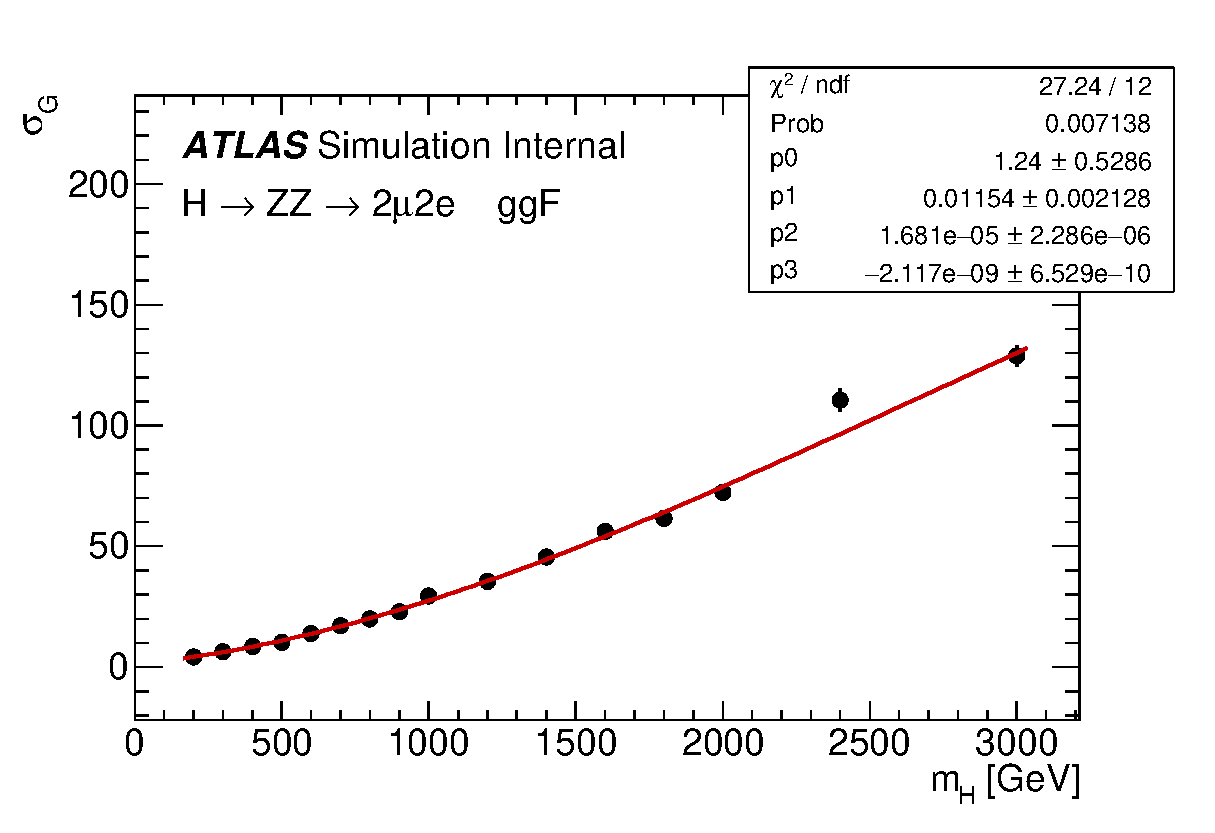
\includegraphics[width=0.32\textwidth]{figures/HMHZZ/signal/NWA//ggf_graph_mass_gauss_sigma_2mu2e_fit.eps} \\
    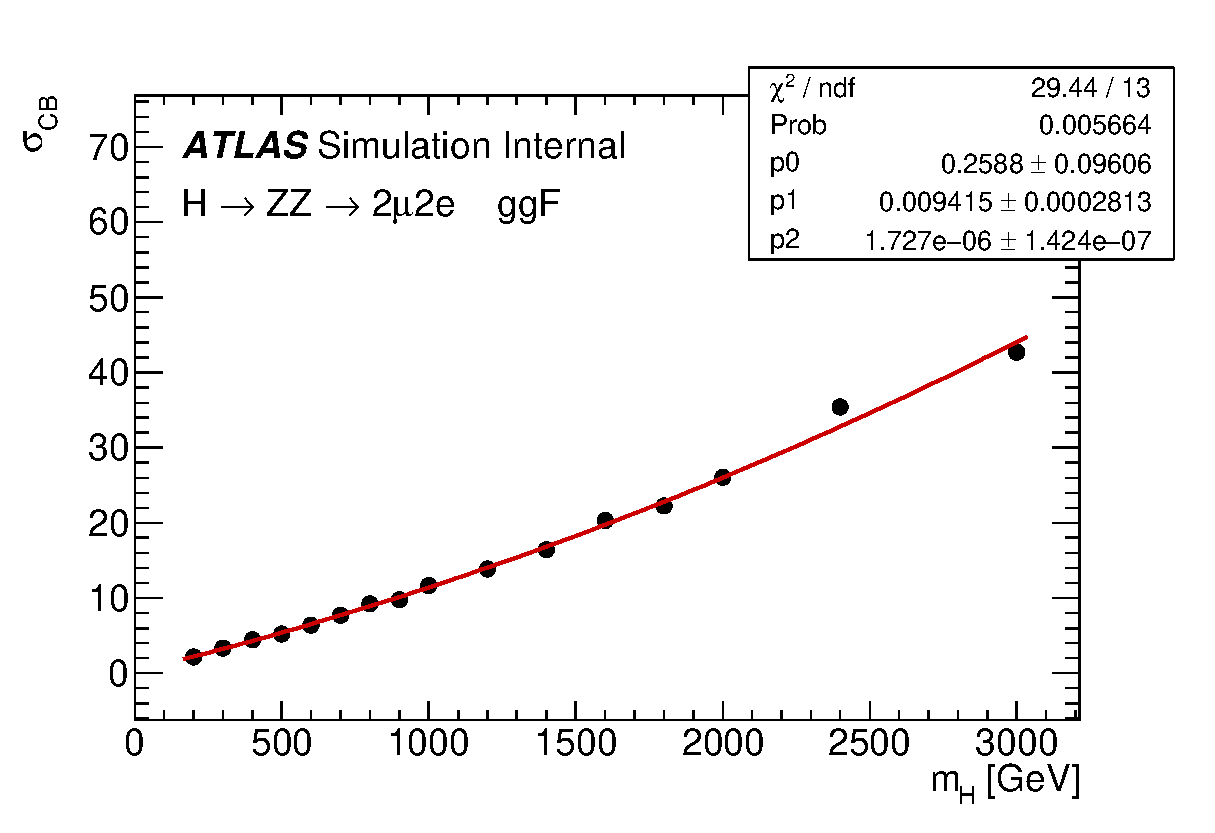
\includegraphics[width=0.32\textwidth]{figures/HMHZZ/signal/NWA//ggf_graph_mass_cb_sigma_2mu2e_fit.eps}
    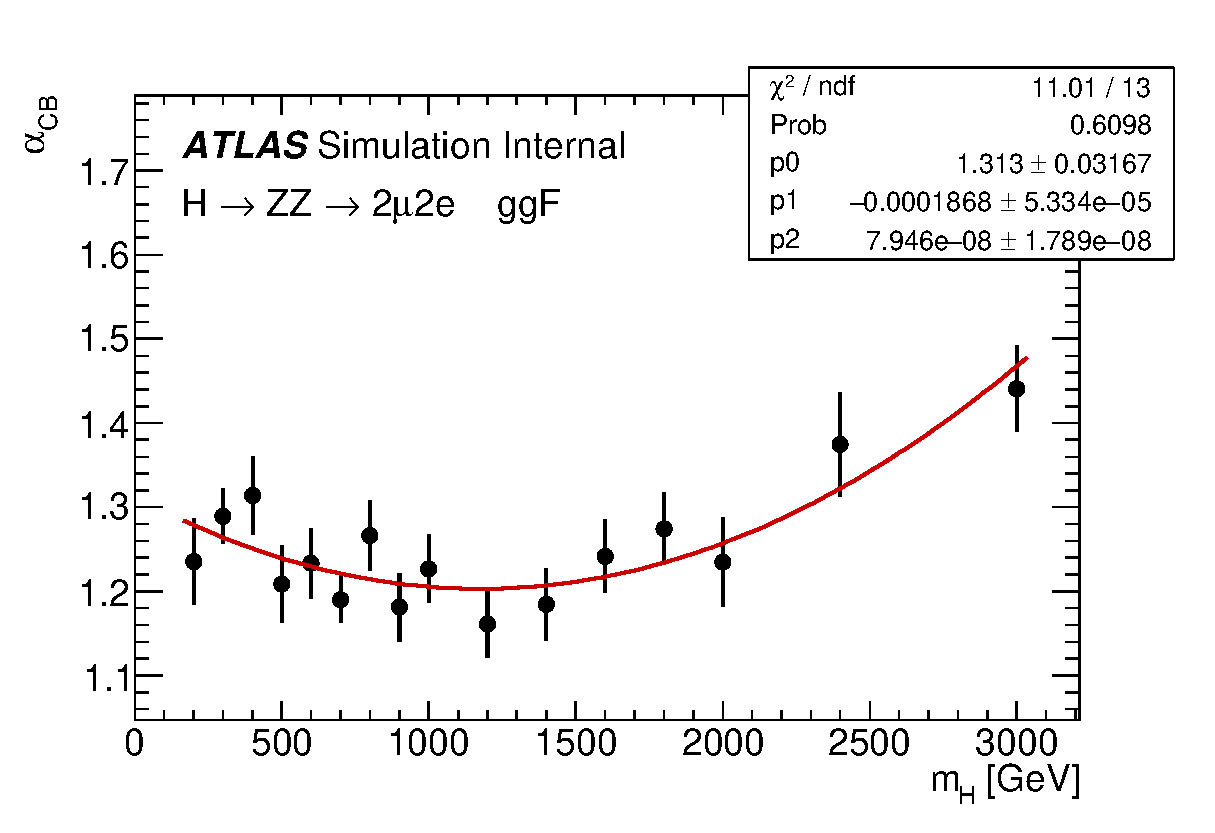
\includegraphics[width=0.32\textwidth]{figures/HMHZZ/signal/NWA//ggf_graph_mass_cb_alpha_2mu2e_fit.eps}
    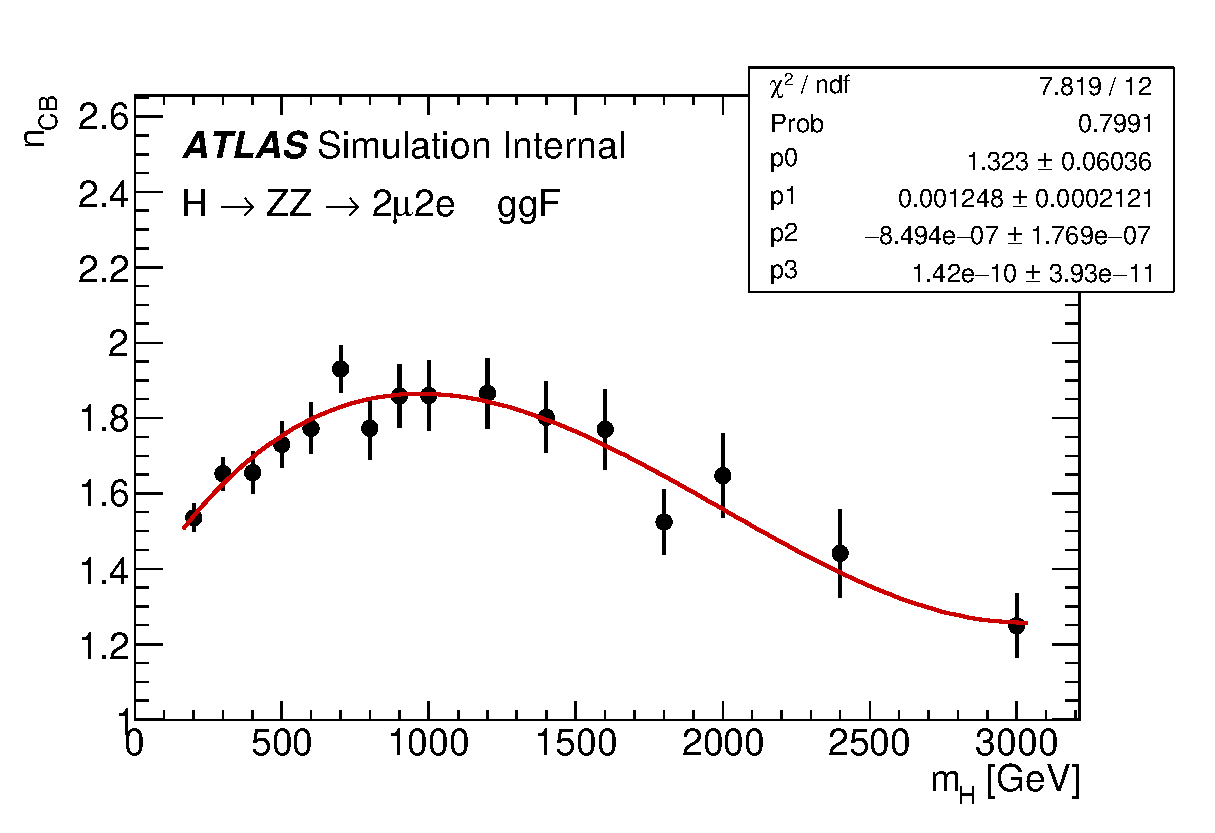
\includegraphics[width=0.32\textwidth]{figures/HMHZZ/signal/NWA//ggf_graph_mass_cb_n_2mu2e_fit.eps}
    \caption{Polynomial fits of the parameters $\mu$, $f_{\mathcal{C}}$, $\sigma_{\mathcal{G}}$, $\sigma_{\mathcal{C}}$,
    $n_{\mathcal{C}}$ and $\alpha_{\mathcal{C}}$ for the signal $\mathcal{C}+\mathcal{G}$ model in the $2\mu 2e$ channel as a function of \mH for
    the ggF production mode. The combination of the mc16a, mc16d and mc16e MC campaigns is used.}
    \label{fig:ggf_fitParams_interpolation_2mu2e}
\end{figure}

In addition, possible difference on the signal yield extracted from parameterization and MC simulation is studied.
Figure~\ref{fig:ggf_graph_YieldCheckAll} shows this difference by computing $\frac{N_{\text{reco}}-N_{\text{fit}}}{N_{\text{fit}}}$, where $N_{\text{reco}}$ denotes the total number of reconstructed events observed from MC simulation at that mass point
and $N_{\text{fit}}$ depicts the number of events obtained from the fitted pdf.
The differences are treated as an additional systematic uncertainty with the value of 2\% (1\%) for 2$e$2$\mu$ (4$e$ and 4$\mu$) channel in statistical fit.

\begin{figure}[htbp]
    \centering
    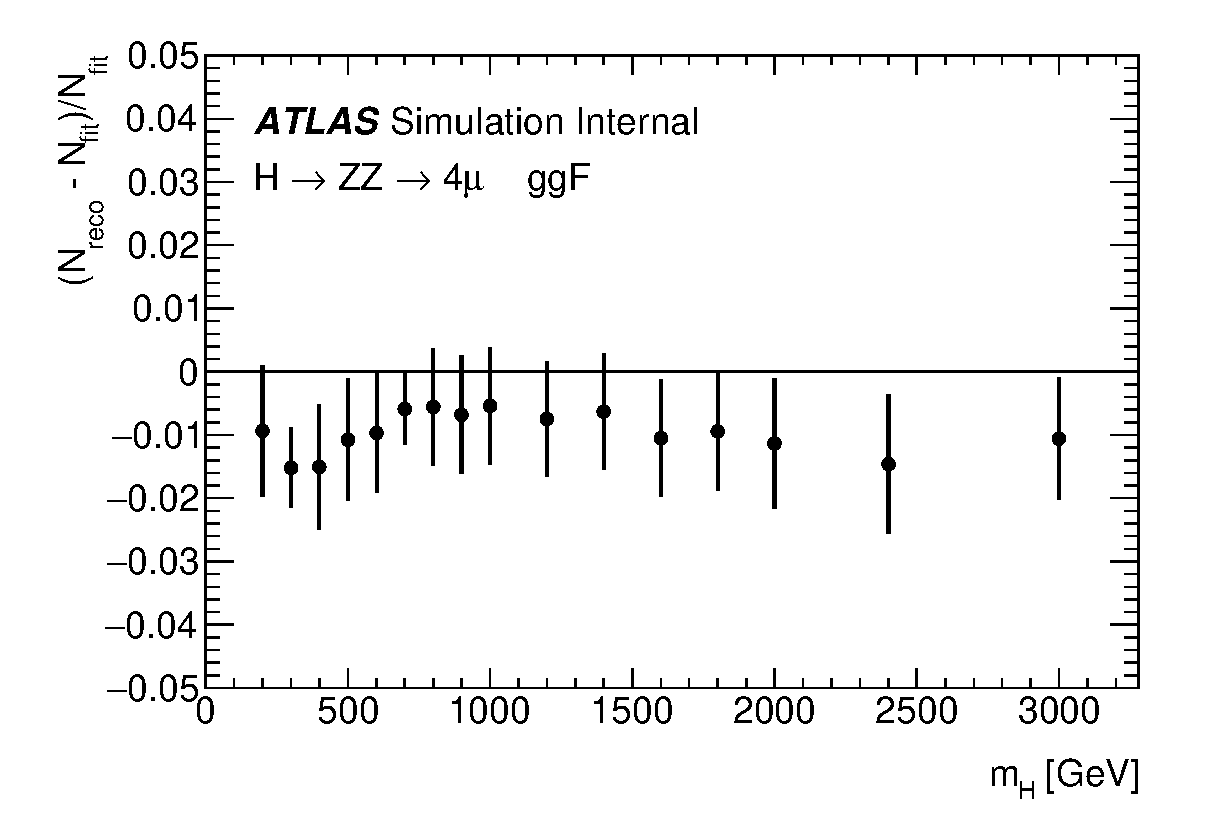
\includegraphics[width=0.32\textwidth]{figures/HMHZZ/signal/NWA//ggf_graph_YieldCheck_4mu_fixed.eps}
    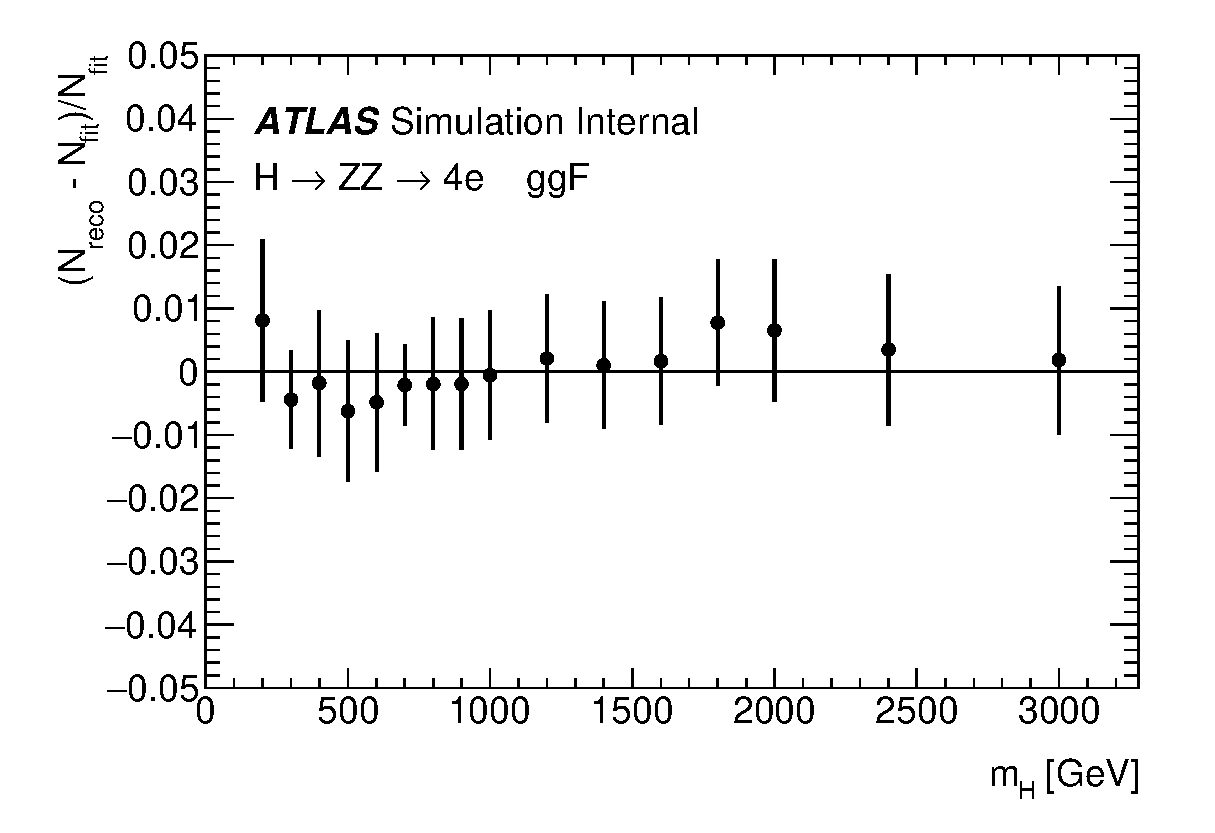
\includegraphics[width=0.32\textwidth]{figures/HMHZZ/signal/NWA//ggf_graph_YieldCheck_4e_fixed.eps}
    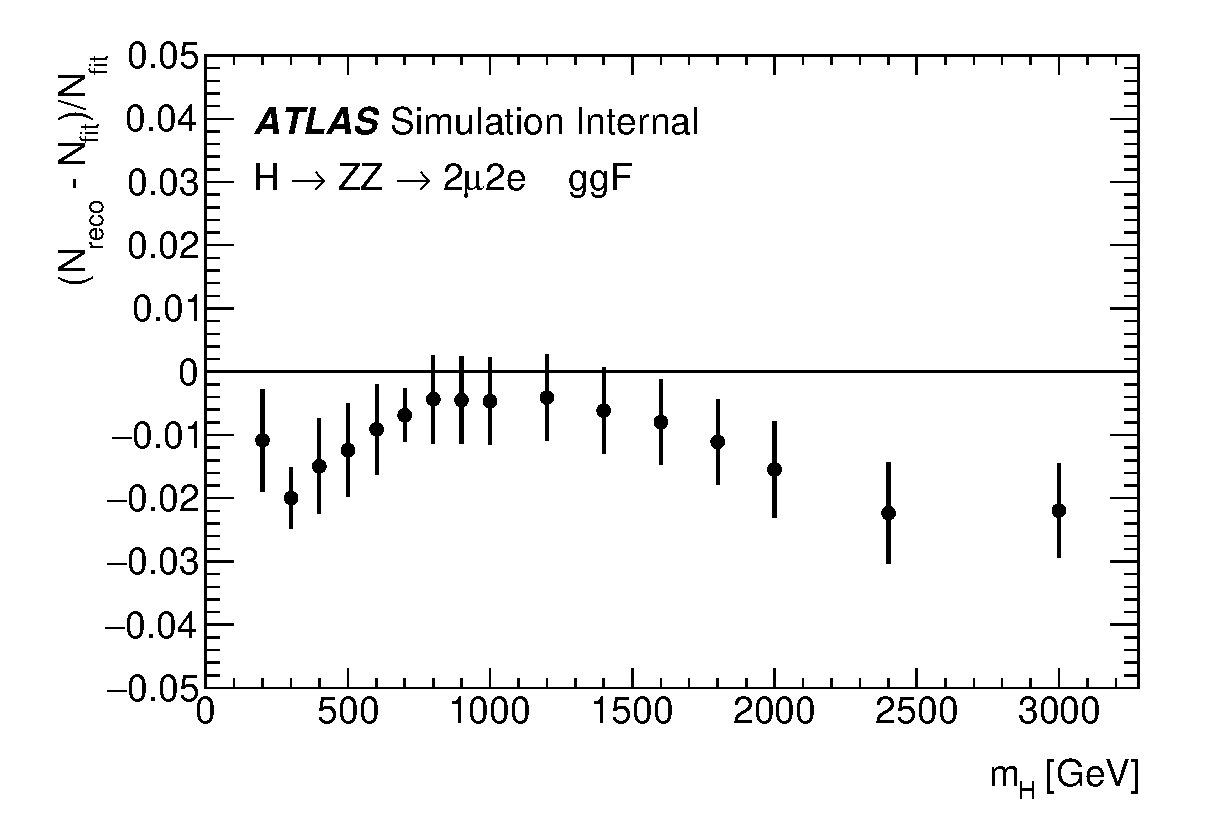
\includegraphics[width=0.32\textwidth]{figures/HMHZZ/signal/NWA//ggf_graph_YieldCheck_2mu2e_fixed.eps}
    \caption{The difference between MC simulation and parameterization of
    $4\mu$ (left), $4e$ (middle) and $2\mu 2e$ (right) for the ggF production
    mode. The combination of the mc16a, mc16d and mc16e MC campaigns is used.}
    \label{fig:ggf_graph_YieldCheckAll}
\end{figure}

In summary, the final interpolated signal shapes for the ggF production mode are shown together in figure~\ref{fig:ggf_multipeak} for mass points with step of 100~\gev~ from 200~\gev~ to 3000~\gev.

\begin{figure}[htbp]
    \centering
    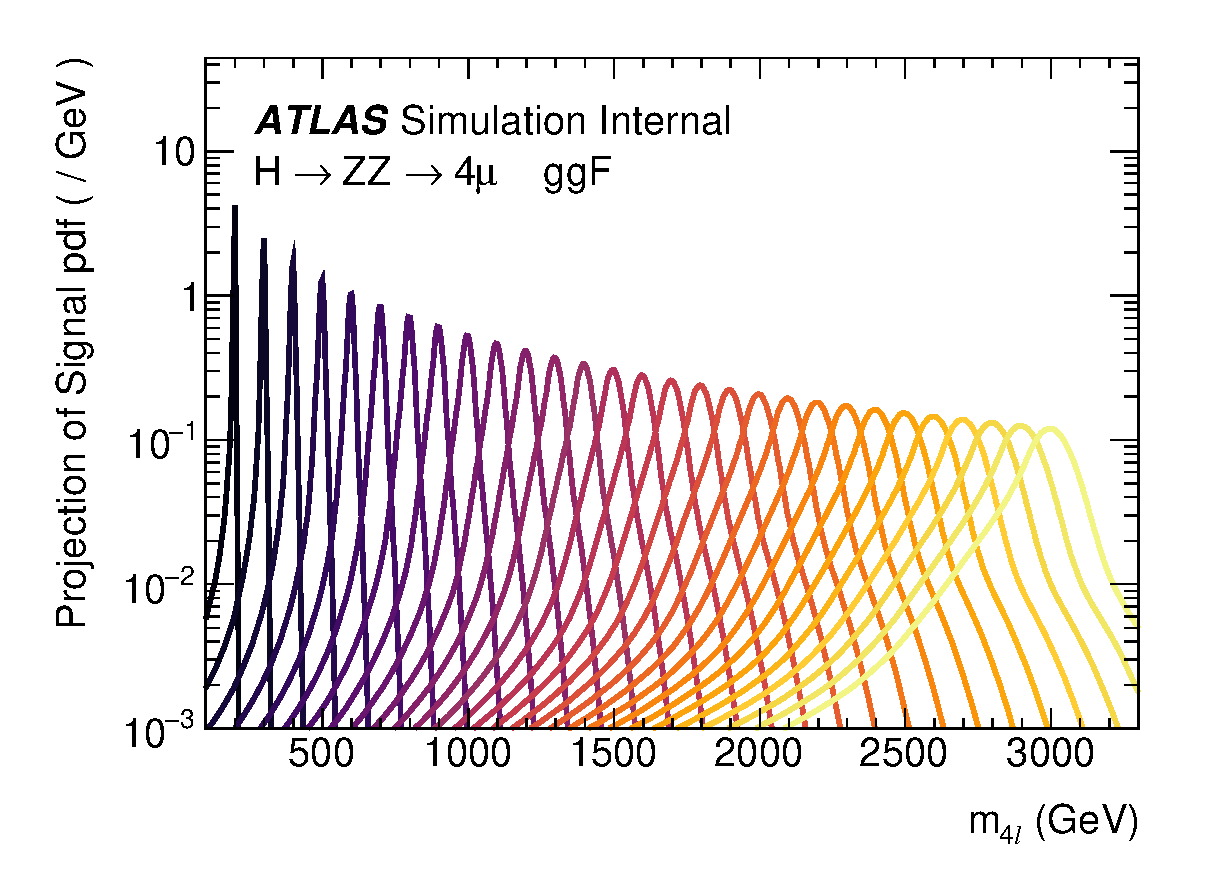
\includegraphics[width=0.32\textwidth]{figures/HMHZZ/signal/NWA//ggf_multipeakplot_4mu.eps}
    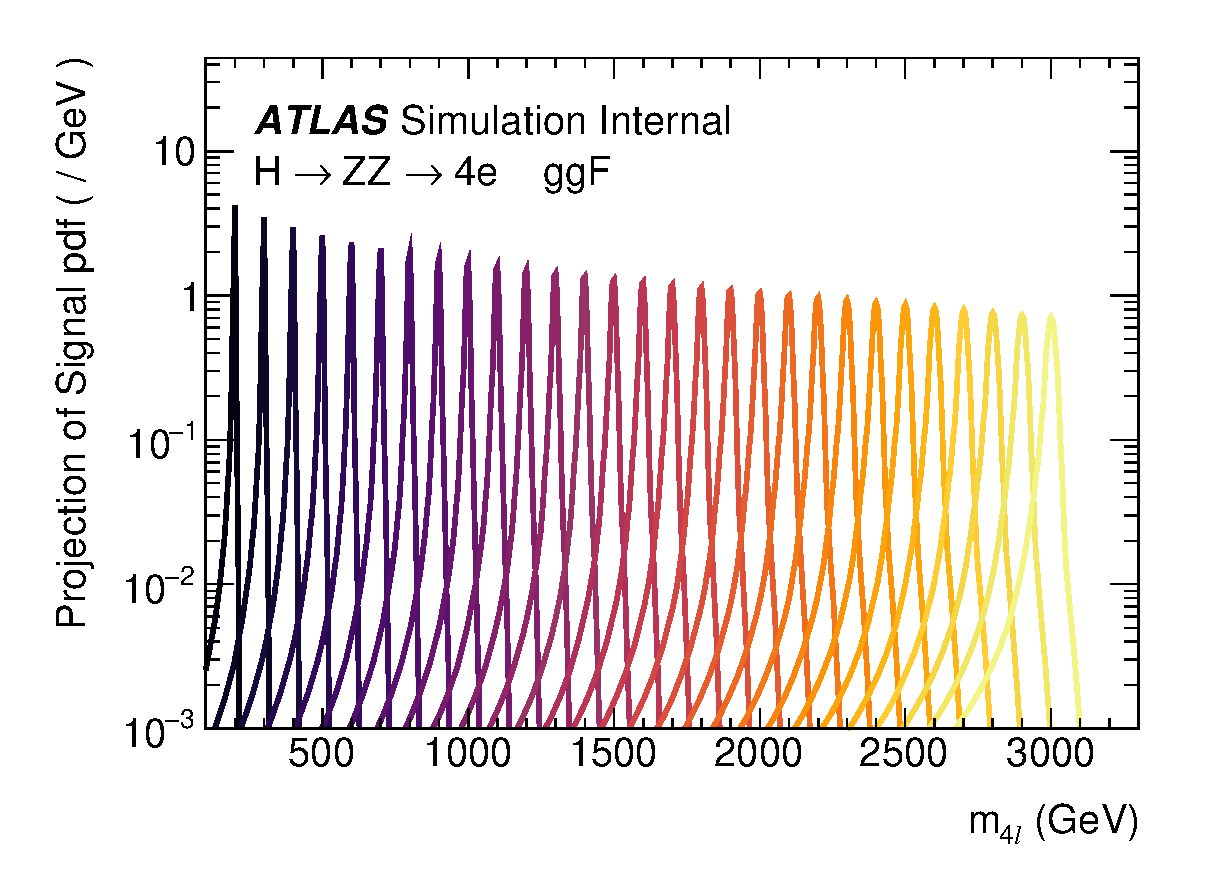
\includegraphics[width=0.32\textwidth]{figures/HMHZZ/signal/NWA//ggf_multipeakplot_4e.eps}
    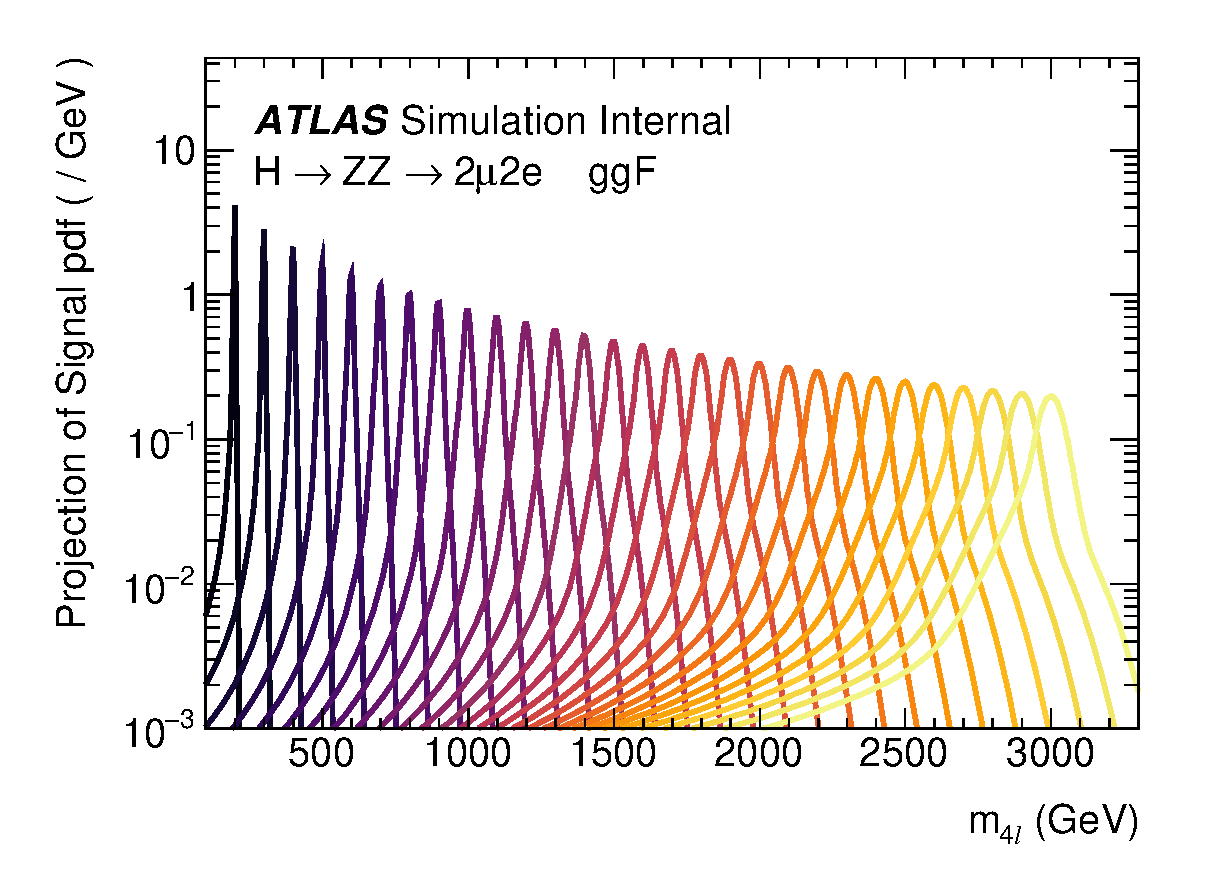
\includegraphics[width=0.32\textwidth]{figures/HMHZZ/signal/NWA//ggf_multipeakplot_2mu2e.eps}
    \caption{The final signal shapes for the ggF production mode, interpolated from the polynomial fit parameters.}
    \label{fig:ggf_multipeak}
\end{figure}

%%========================================================================================================================
%% LWA

\subsection{Modelling of large-width signal}
\label{sec:signal_lwa}

The \mfl shape of heavy Higgs model in large-width (LWA) hypothesis can be described by a convolution of a truth distribution and a resolution from detector effect.
The detector resolution effect is the one modelled by the function described in NWA parameterization, as in NWA model the truth level width is negligible.

The differential parton cross section for the heavy Higgs model can be written as~\cite{Goria:2011wa}:
\begin{equation}
    \sigma_{gg \to H \to ZZ} (s) = \frac{1}{2s}  \int d \Omega \left | A_{gg \to H}(s,\Omega) \right |^2 \frac{1}{ \left | s - s_H \right |^2}  \left | A_{H \to ZZ}(s,\Omega) \right |^2
\end{equation}
where $A_{gg \to H}(s,\Omega)$ and $A_{H \to ZZ}(s,\Omega)$ are corresponding Higgs production and decay amplitudes,
and $\frac{1}{s - s_H}$ denotes the Higgs propagator and $\Omega$ represents the phase space of the process.

Using the definition of a partial width,
\begin{equation} \label{eq:PartialWidth}
    \Gamma_{H \to F} (s) = \frac{1}{2\sqrt{s}}  \int d \Omega \left | A_{H \to F}(s,\Omega) \right |^2
\end{equation}
the parton cross section can be rewritten as,
\begin{equation} \label{eq:HiggsPartonXSection}
    \sigma_{gg \to H \to ZZ} (s) = 2 \frac{1}{ \left | s - s_H \right |^2}  \times \Gamma_{H \to gg} (s) \times \Gamma_{H \to ZZ} (s)
\end{equation}
with the components computed in Ref~\cite{Goria:2011wa,Spira1995}:
\begin{align} \label{eq:propagator}
\begin{split}
    \frac{1}{s - s_H} &= \frac{ 1 + i \cdot \overline{\Gamma}_H / \overline{m}_H} { s - \overline{m}_H^2 +  i \cdot s \cdot\overline{\Gamma}_H / \overline{m}_H }  \\
    \overline{m}_H &= \sqrt{\Gamma_H^2 + m_H^2} \\
    \overline{\Gamma}_H &= \overline{m}_H  \cdot \frac{\Gamma_H}{m_H}
\end{split}
\end{align}

\begin{equation} \label{eq:WidthZZ}
    \Gamma_{H \to ZZ} (s) = C \cdot s^{\frac{3}{2}} \cdot \left [ 1 - \frac{4m_Z^2}{s} + \frac{3}{4}\left ( \frac{4m_Z^2}{s} \right )^2 \right ] \cdot \left [ 1 - \frac{4m_Z^2}{s} \right ]^{\frac{1}{2}}
\end{equation}

\begin{align} \label{eq:WidthGG}
\begin{split}
    \Gamma_{H \to gg} (s) &= C \cdot s^{\frac{3}{2}} \cdot \left | A_t(\tau_t) \right |^{2} \\
    A_t(\tau) &= 2 \frac{\tau+(\tau-1)f(\tau)}{\tau^2} \\
    \tau_t &= \frac{s}{4m_t^2} \\
    f(\tau) &= \left\{\begin{matrix}
    \arcsin^2 (\sqrt{\tau}) , ~ \tau \leqslant 1
    \\
    - \frac{1}{4} \left [  \log{\frac{1+\sqrt{1-\tau^{-1}}}{1-\sqrt{1-\tau^{-1}}}}  - i  \pi \right ]^2 , ~ \tau > 1
    \end{matrix}\right.
\end{split}
\end{align}

where $m_f$ stands for the mass of a fermion $f$, and $\Gamma_H$ denotes an assumed total width of the heavy Higgs boson.

At the LHC, the \mfl line shape can be defined by a hadron cross section that is derived from
equation~\ref{eq:HiggsPartonXSection} by multiplication with gluon-gluon luminosity $\mathcal{L}_{gg}$ described in
\cite{Ball:2012wy}. 
Meanwhile, the cross section is rewritten as a function of \mfl instead of $s$, which will give an extra power of mass dependence in the formula:
\begin{equation} \label{eq:HiggsHadronXSection}
    \sigma_{pp \to H \to ZZ} (m_{4\ell}) = 2 \cdot m_{4\ell} \cdot \mathcal{L}_{gg} \cdot  \frac{1}{ \left | s - s_H \right |^2}  \cdot \Gamma_{H \to gg} (m_{4\ell}^2) \cdot \Gamma_{H \to ZZ} (m_{4\ell}^2)
\end{equation}
The analytical shapes of truth level \mfl distribution of gg2VV MC samples is shown on figure~\ref{fig:truthShape}.

\begin{figure}[!htbp]
    \centering
    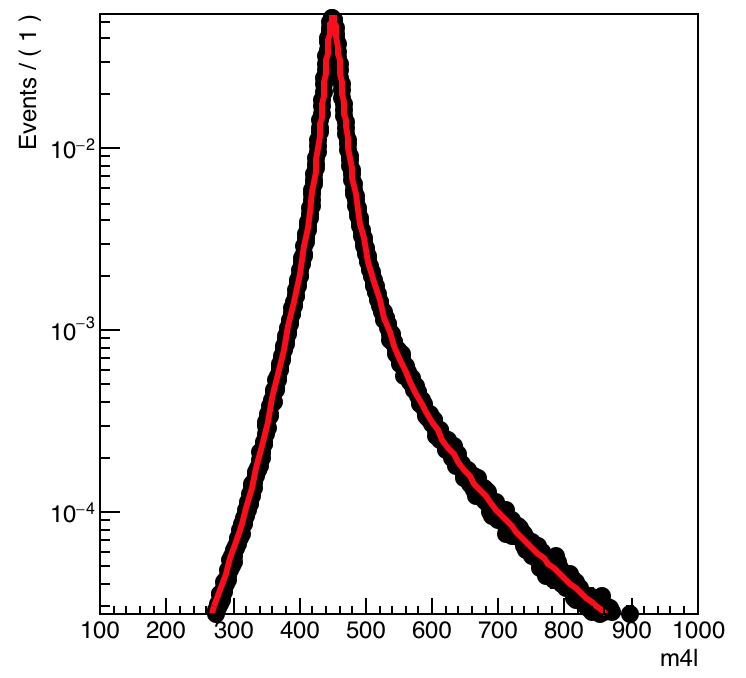
\includegraphics[width=0.32\textwidth]{figures/HMHZZ/signal/LWA/450_5.png}
    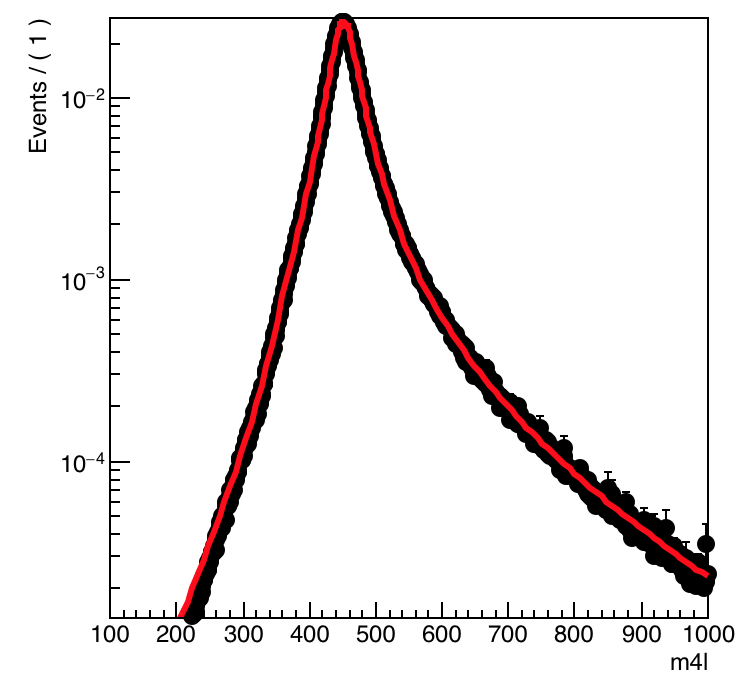
\includegraphics[width=0.32\textwidth]{figures/HMHZZ/signal/LWA/450_10.png}
    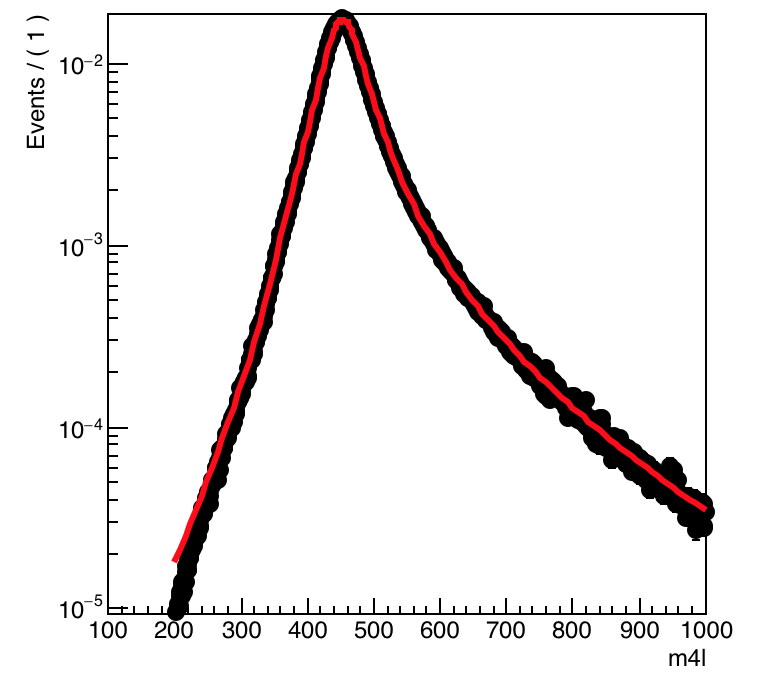
\includegraphics[width=0.32\textwidth]{figures/HMHZZ/signal/LWA/450_15.png}\\
    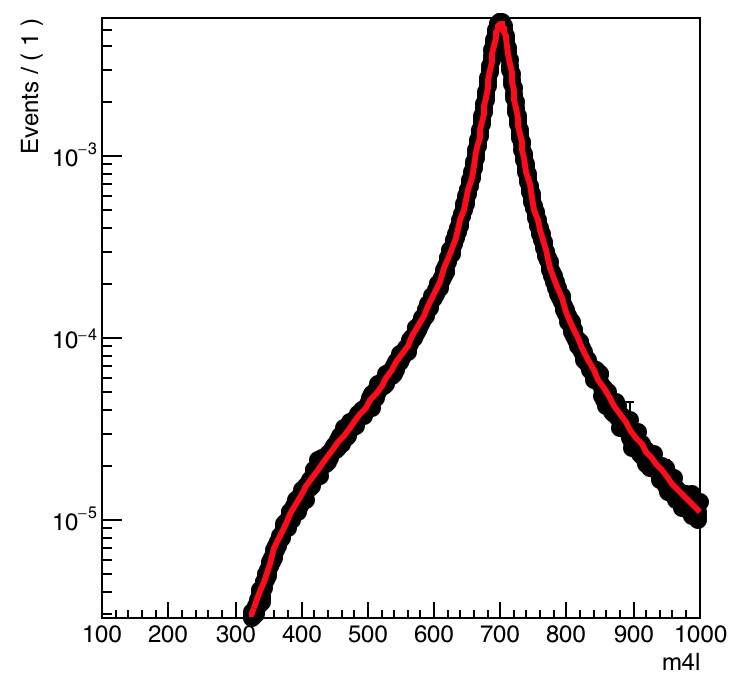
\includegraphics[width=0.32\textwidth]{figures/HMHZZ/signal/LWA/700_5.png}
    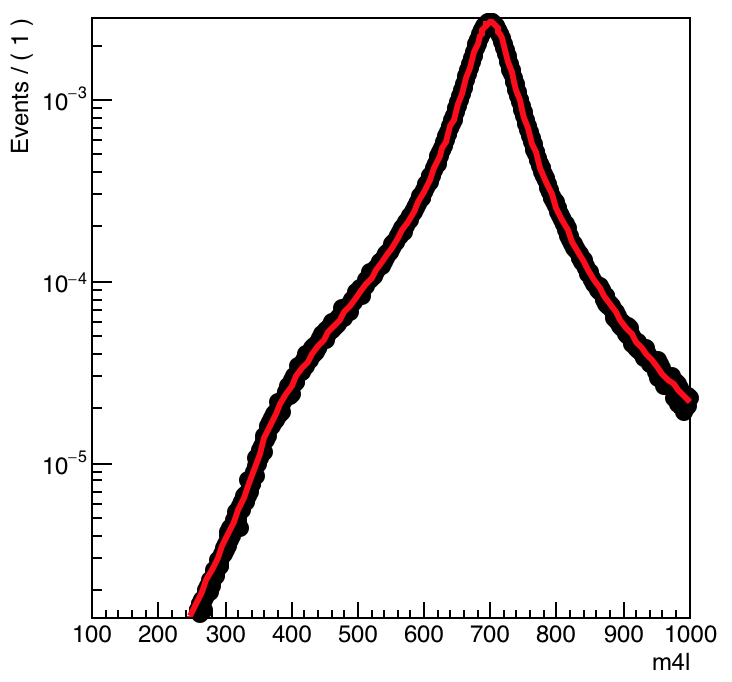
\includegraphics[width=0.32\textwidth]{figures/HMHZZ/signal/LWA/700_10.png}
    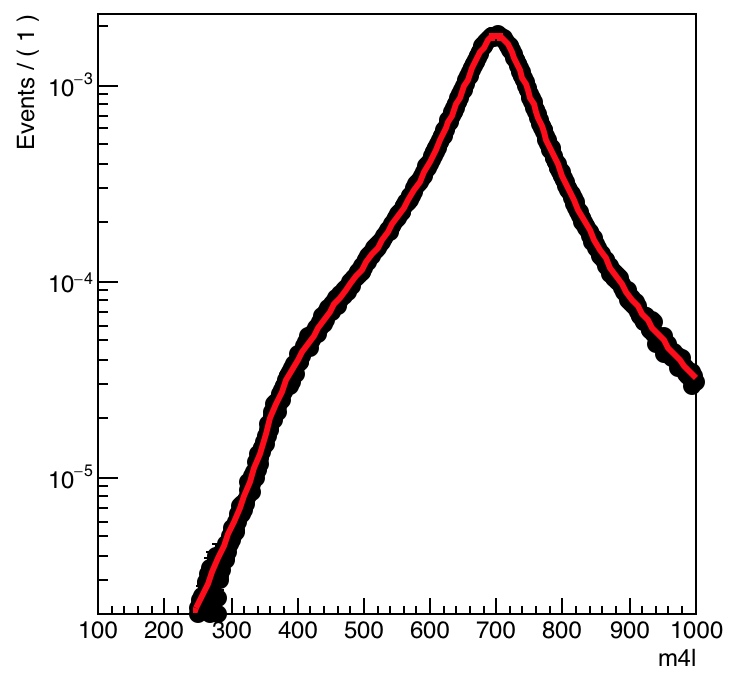
\includegraphics[width=0.32\textwidth]{figures/HMHZZ/signal/LWA/700_15.png}\\
    \caption{Comparison of the analytical shape to a truth $\mfl$ distribution of gg2VV MC samples for $\mH$ = 450~\gev (top), 700~\gev (bottom) 
    and width equal to 5$\%$ (left), 10$\%$ (middle), 15$\%$ (right) of the mass.}
    \label{fig:truthShape}
\end{figure}

The reconstruction level signal shape can then be modelled by the analytical truth shape convoluted with detector effects modelled in section~\ref{sec:signal_nwa}.
A comparison between the modelled shape and reconstruction level MC simulation for signal mass above 400~\gev~ (for ggF production in 2$e$2$\mu$ channel as an example) are shown in figure~\ref{fig:recoShape_2mu2e}, 
the shapes are well compatible between each other.
This modelling is not valid for lower masses due to the rapid change of detector resolution.

\begin{figure}[!htbp]
    \centering
    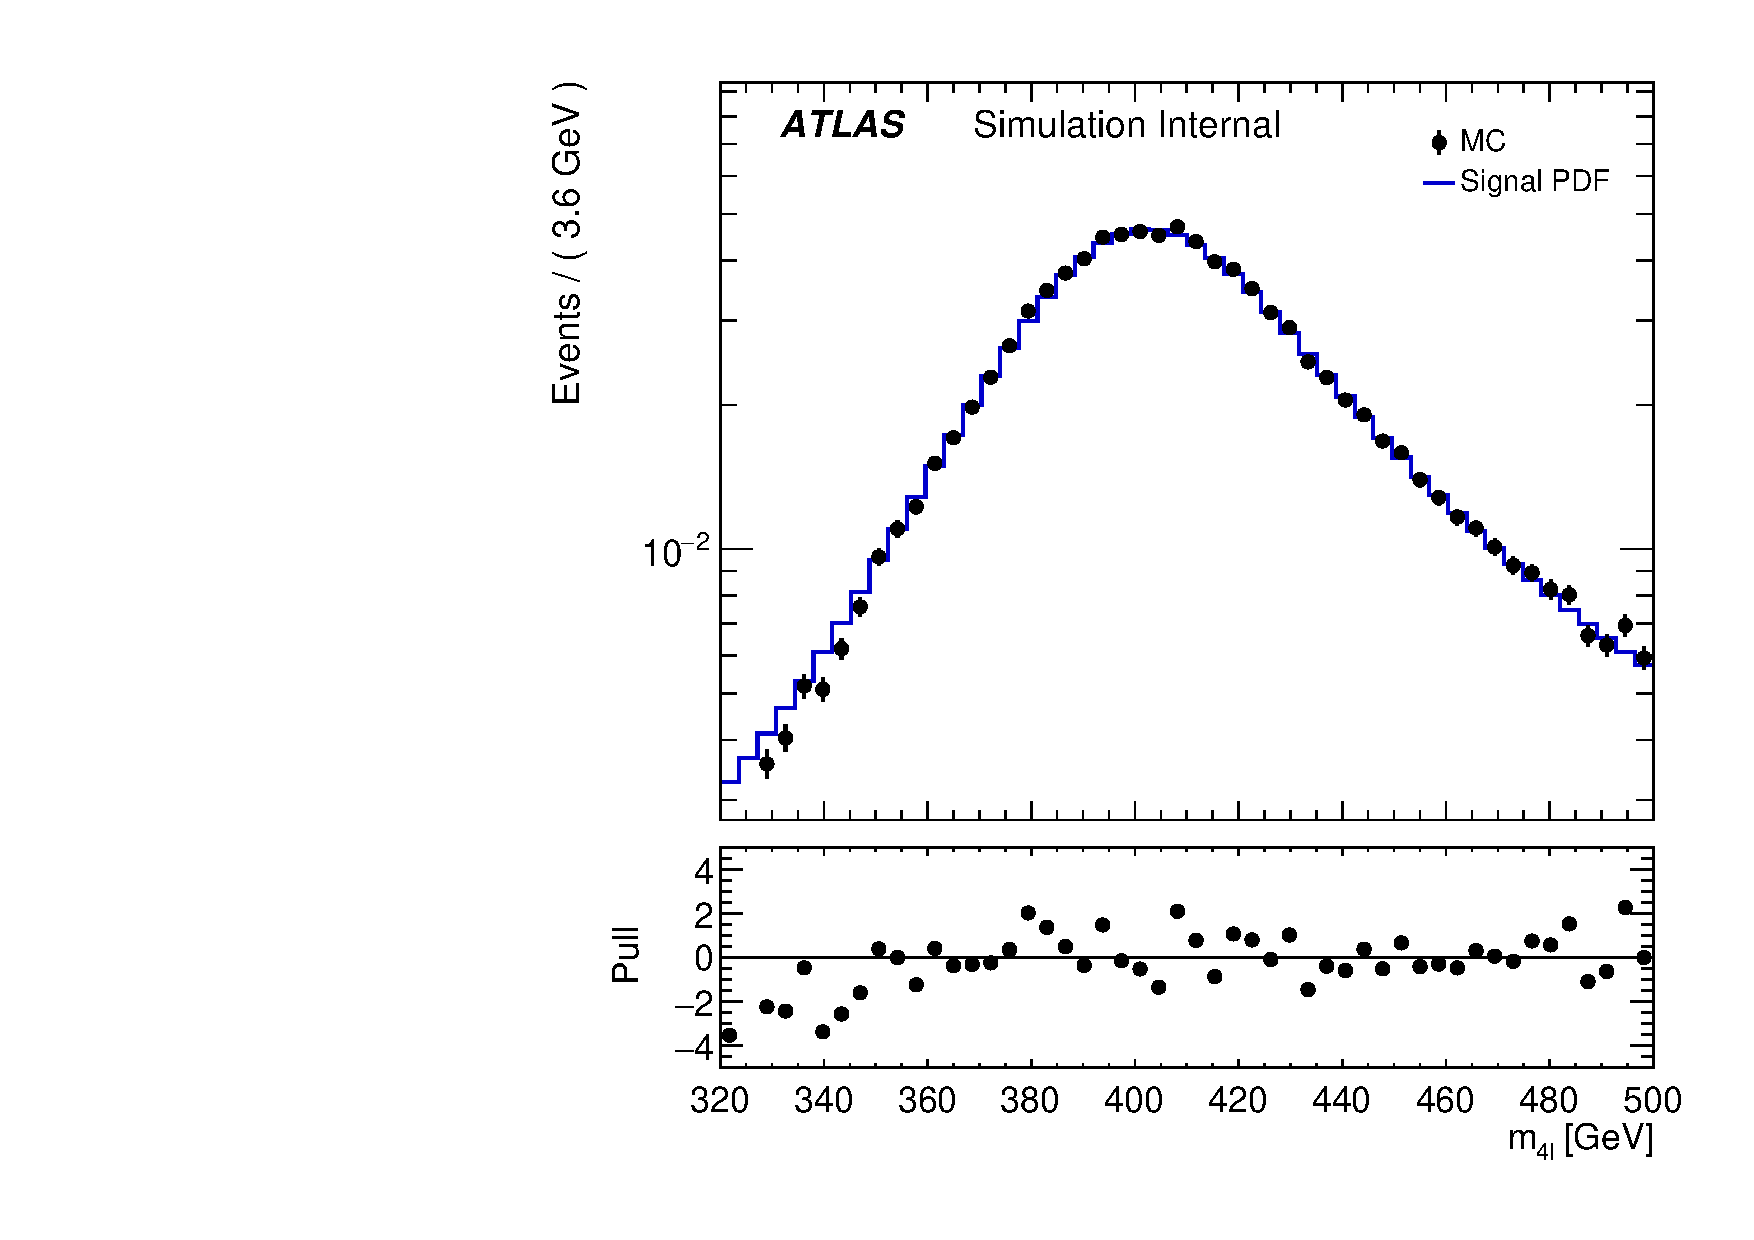
\includegraphics[width=.32\textwidth]{figures/HMHZZ/signal/LWA/cmp_400GeV_ATLAS_Signal_ggF_ggF_2mu2e_13TeV_conv.pdf}
    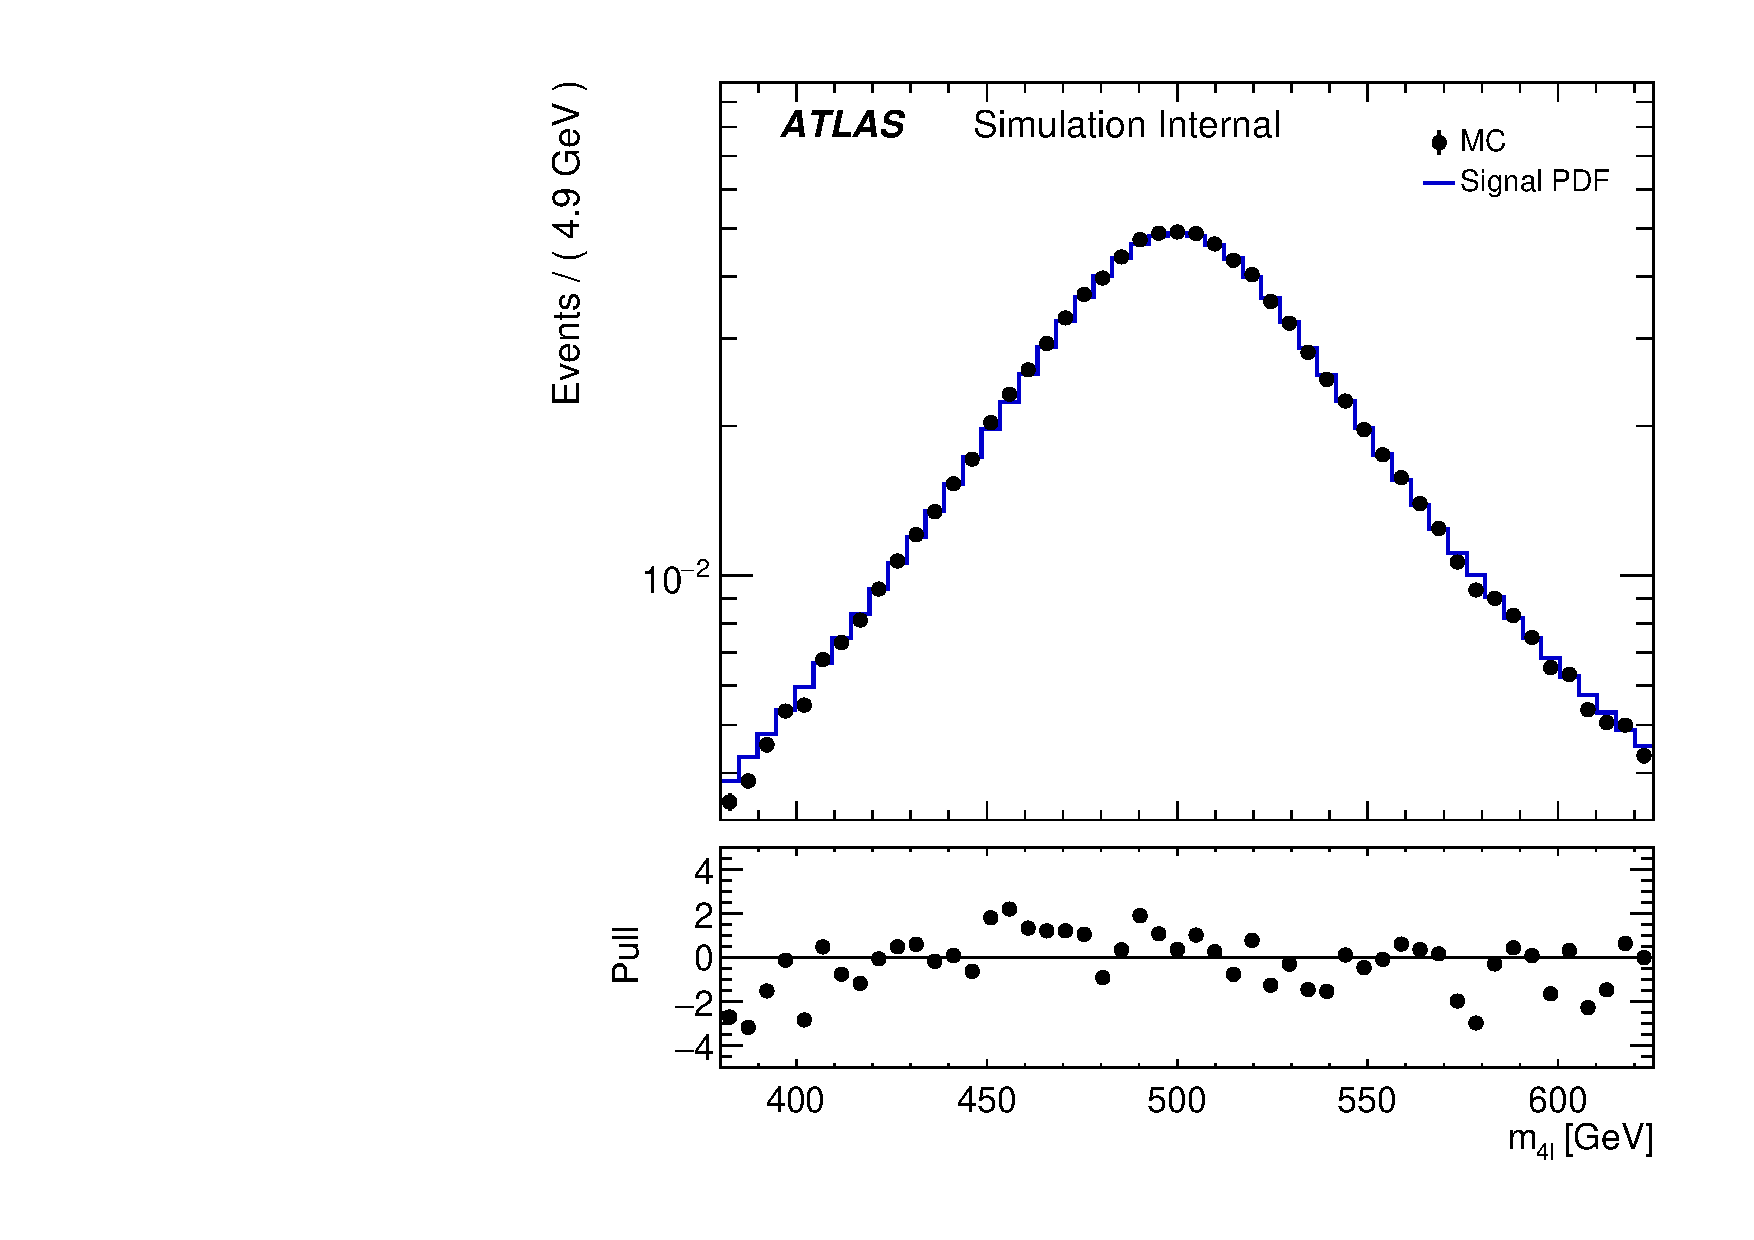
\includegraphics[width=.32\textwidth]{figures/HMHZZ/signal/LWA/cmp_500GeV_ATLAS_Signal_ggF_ggF_2mu2e_13TeV_conv.pdf}
    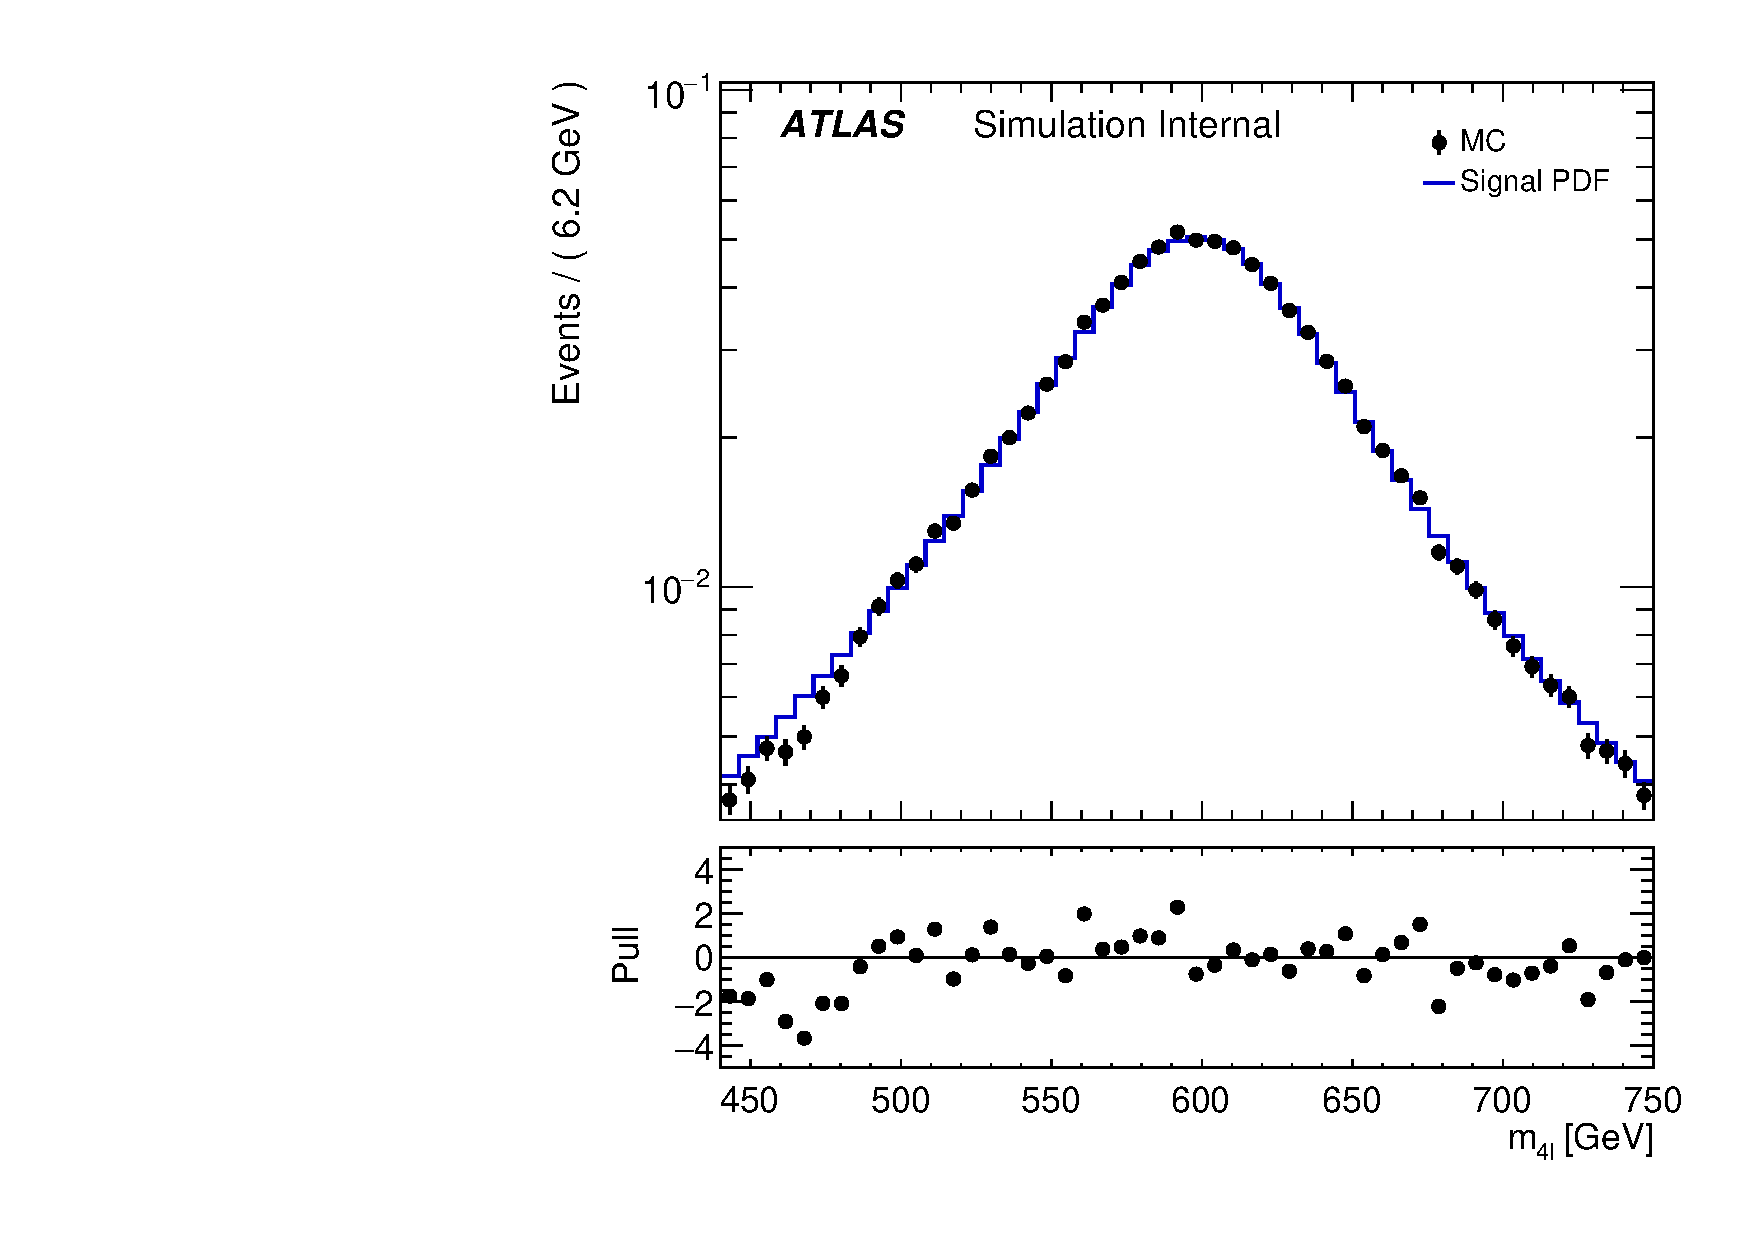
\includegraphics[width=.32\textwidth]{figures/HMHZZ/signal/LWA/cmp_600GeV_ATLAS_Signal_ggF_ggF_2mu2e_13TeV_conv.pdf}\\
    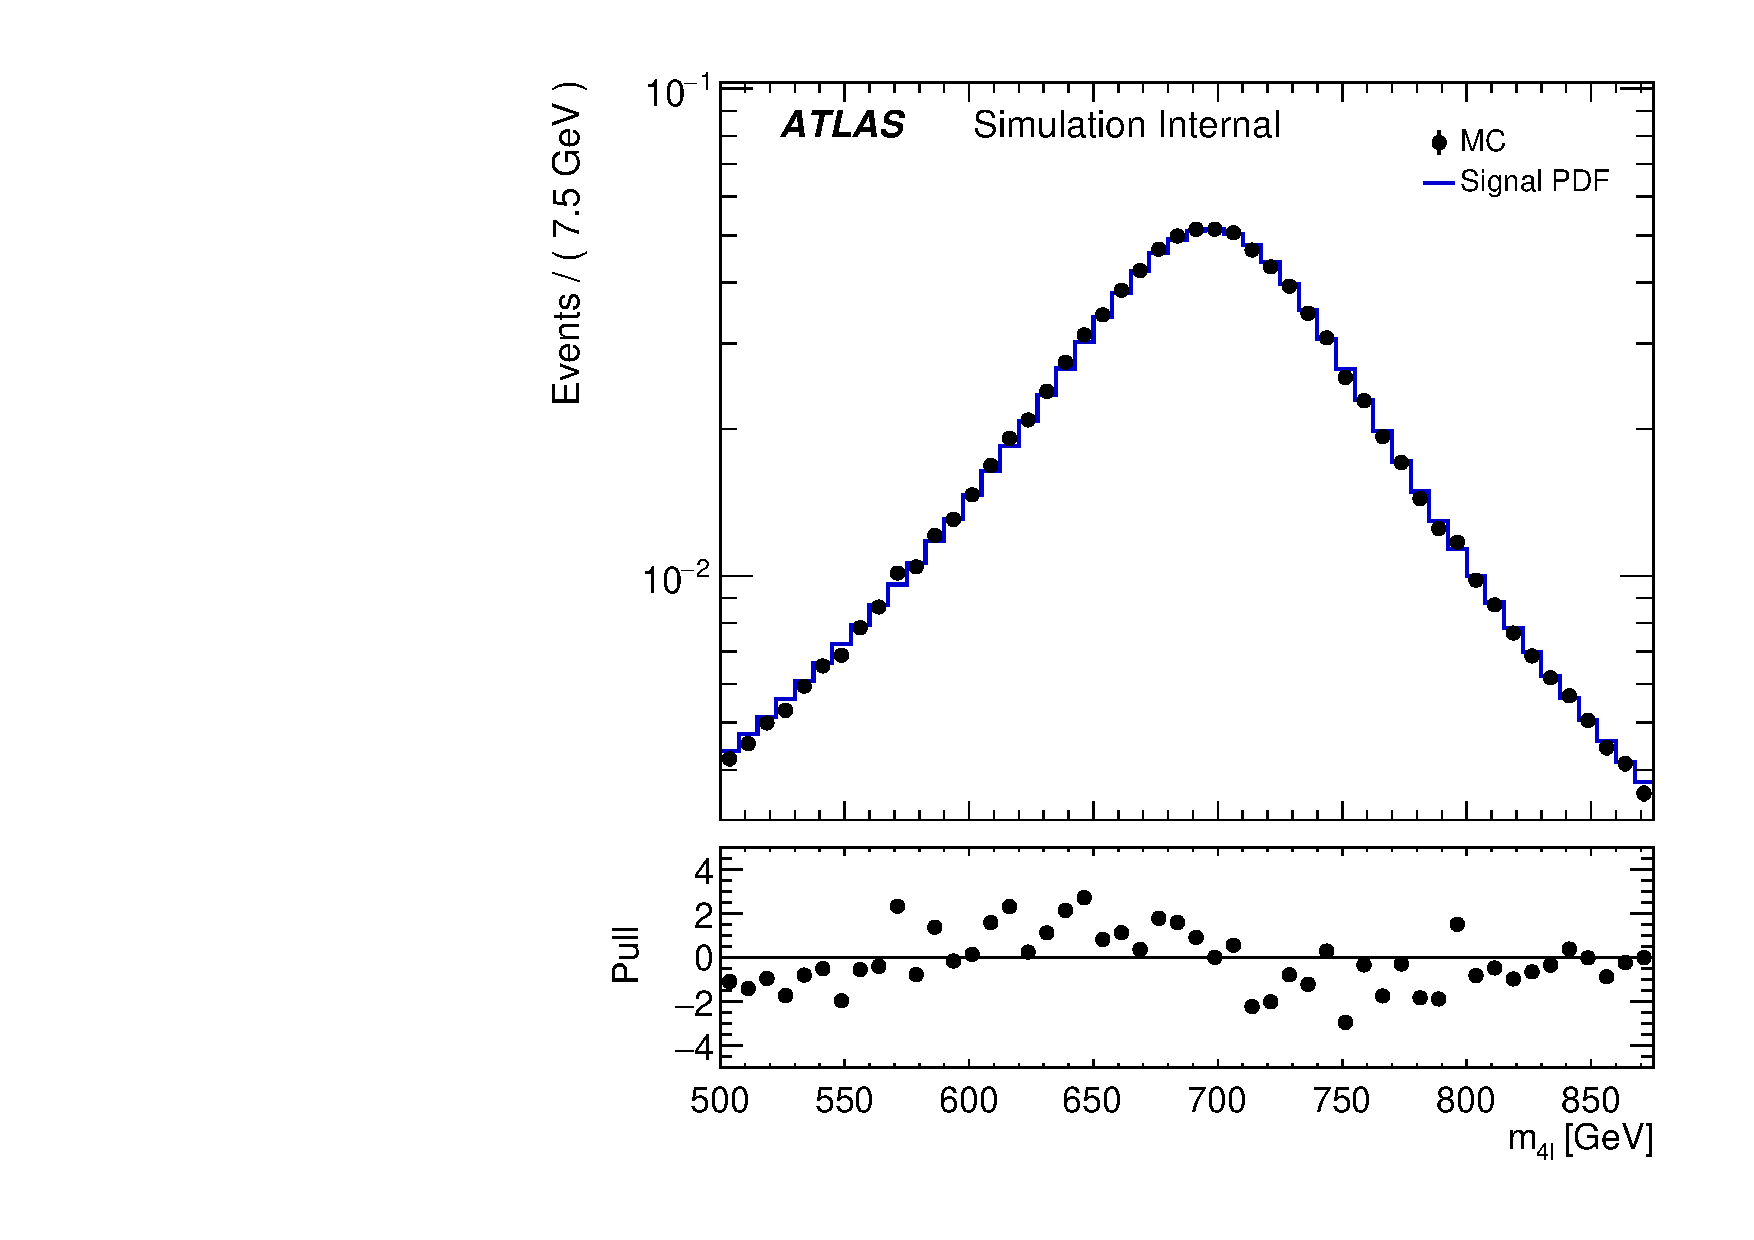
\includegraphics[width=.32\textwidth]{figures/HMHZZ/signal/LWA/cmp_700GeV_ATLAS_Signal_ggF_ggF_2mu2e_13TeV_conv.pdf}
    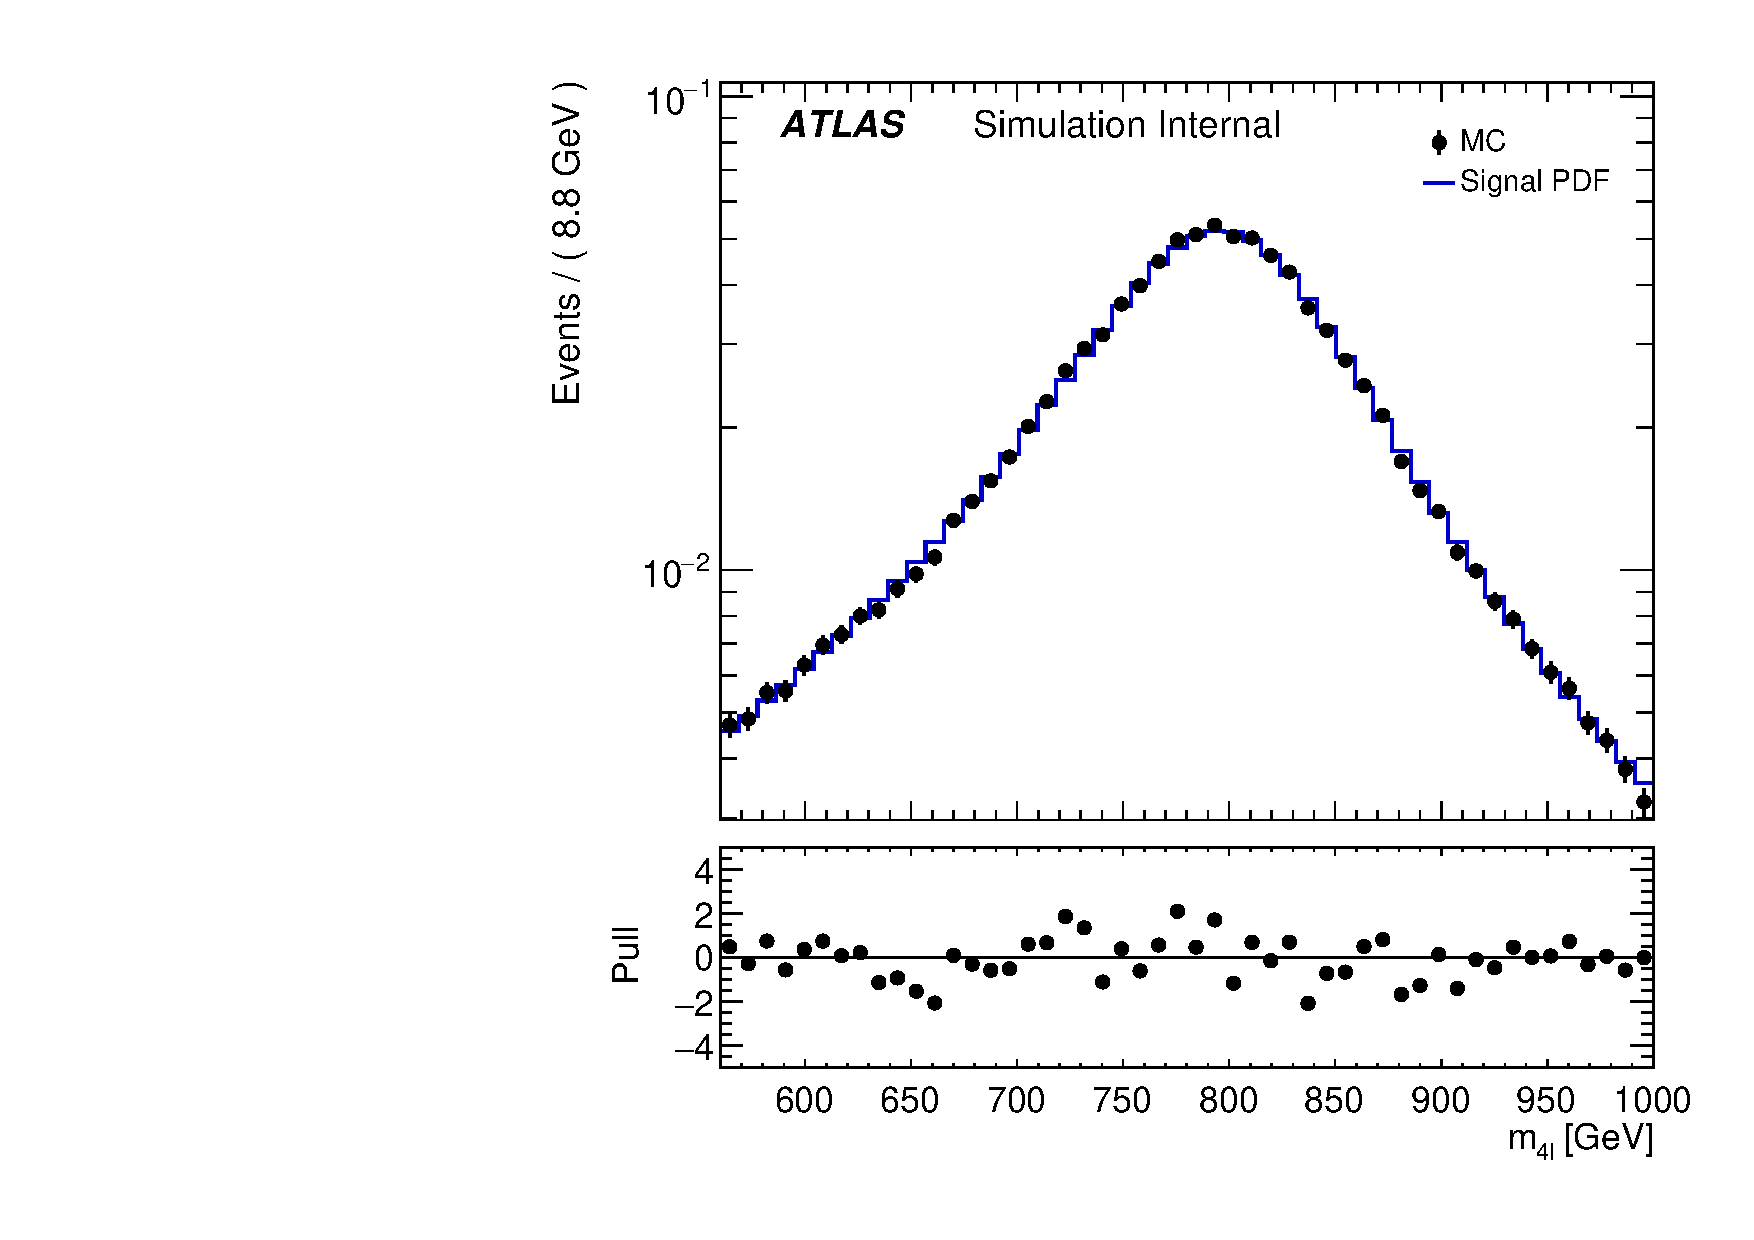
\includegraphics[width=.32\textwidth]{figures/HMHZZ/signal/LWA/cmp_800GeV_ATLAS_Signal_ggF_ggF_2mu2e_13TeV_conv.pdf}
    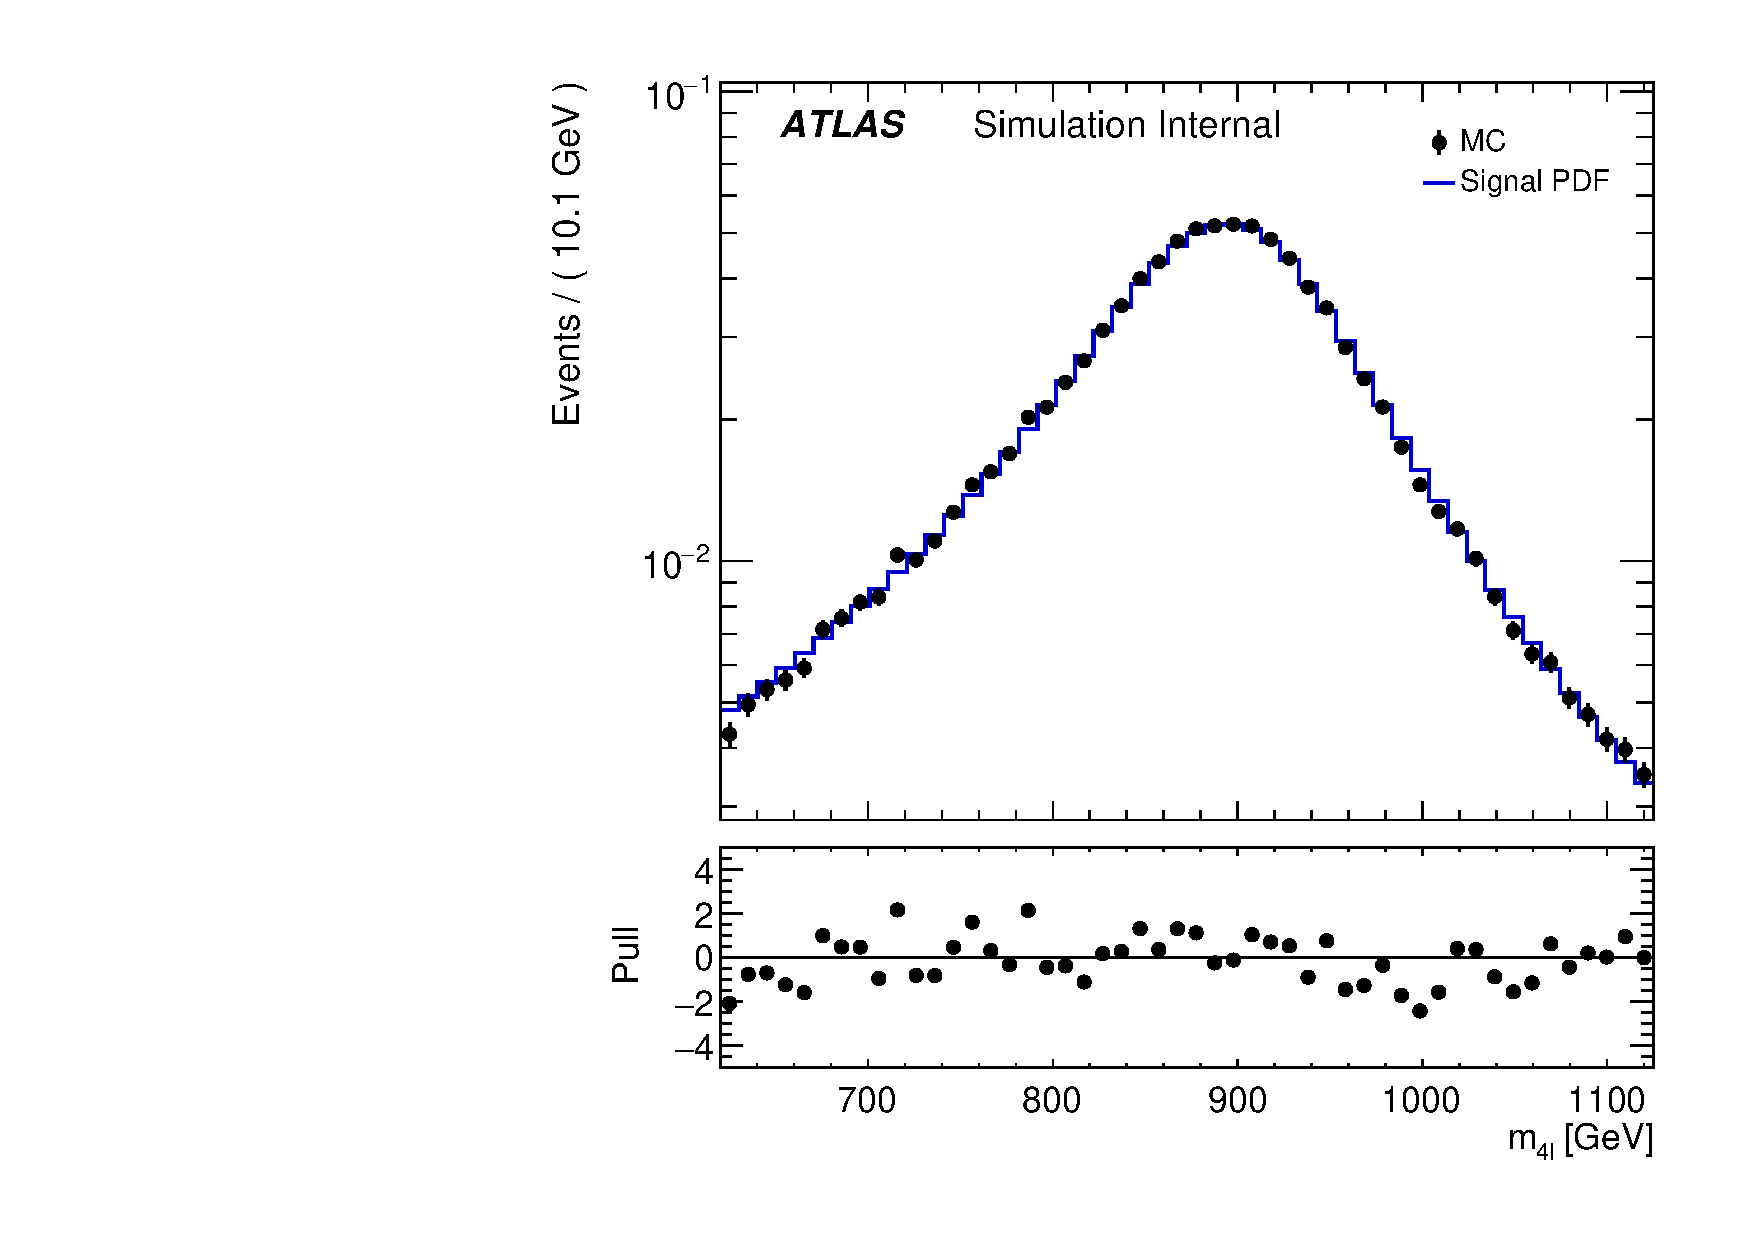
\includegraphics[width=.32\textwidth]{figures/HMHZZ/signal/LWA/cmp_900GeV_ATLAS_Signal_ggF_ggF_2mu2e_13TeV_conv.pdf}\\
    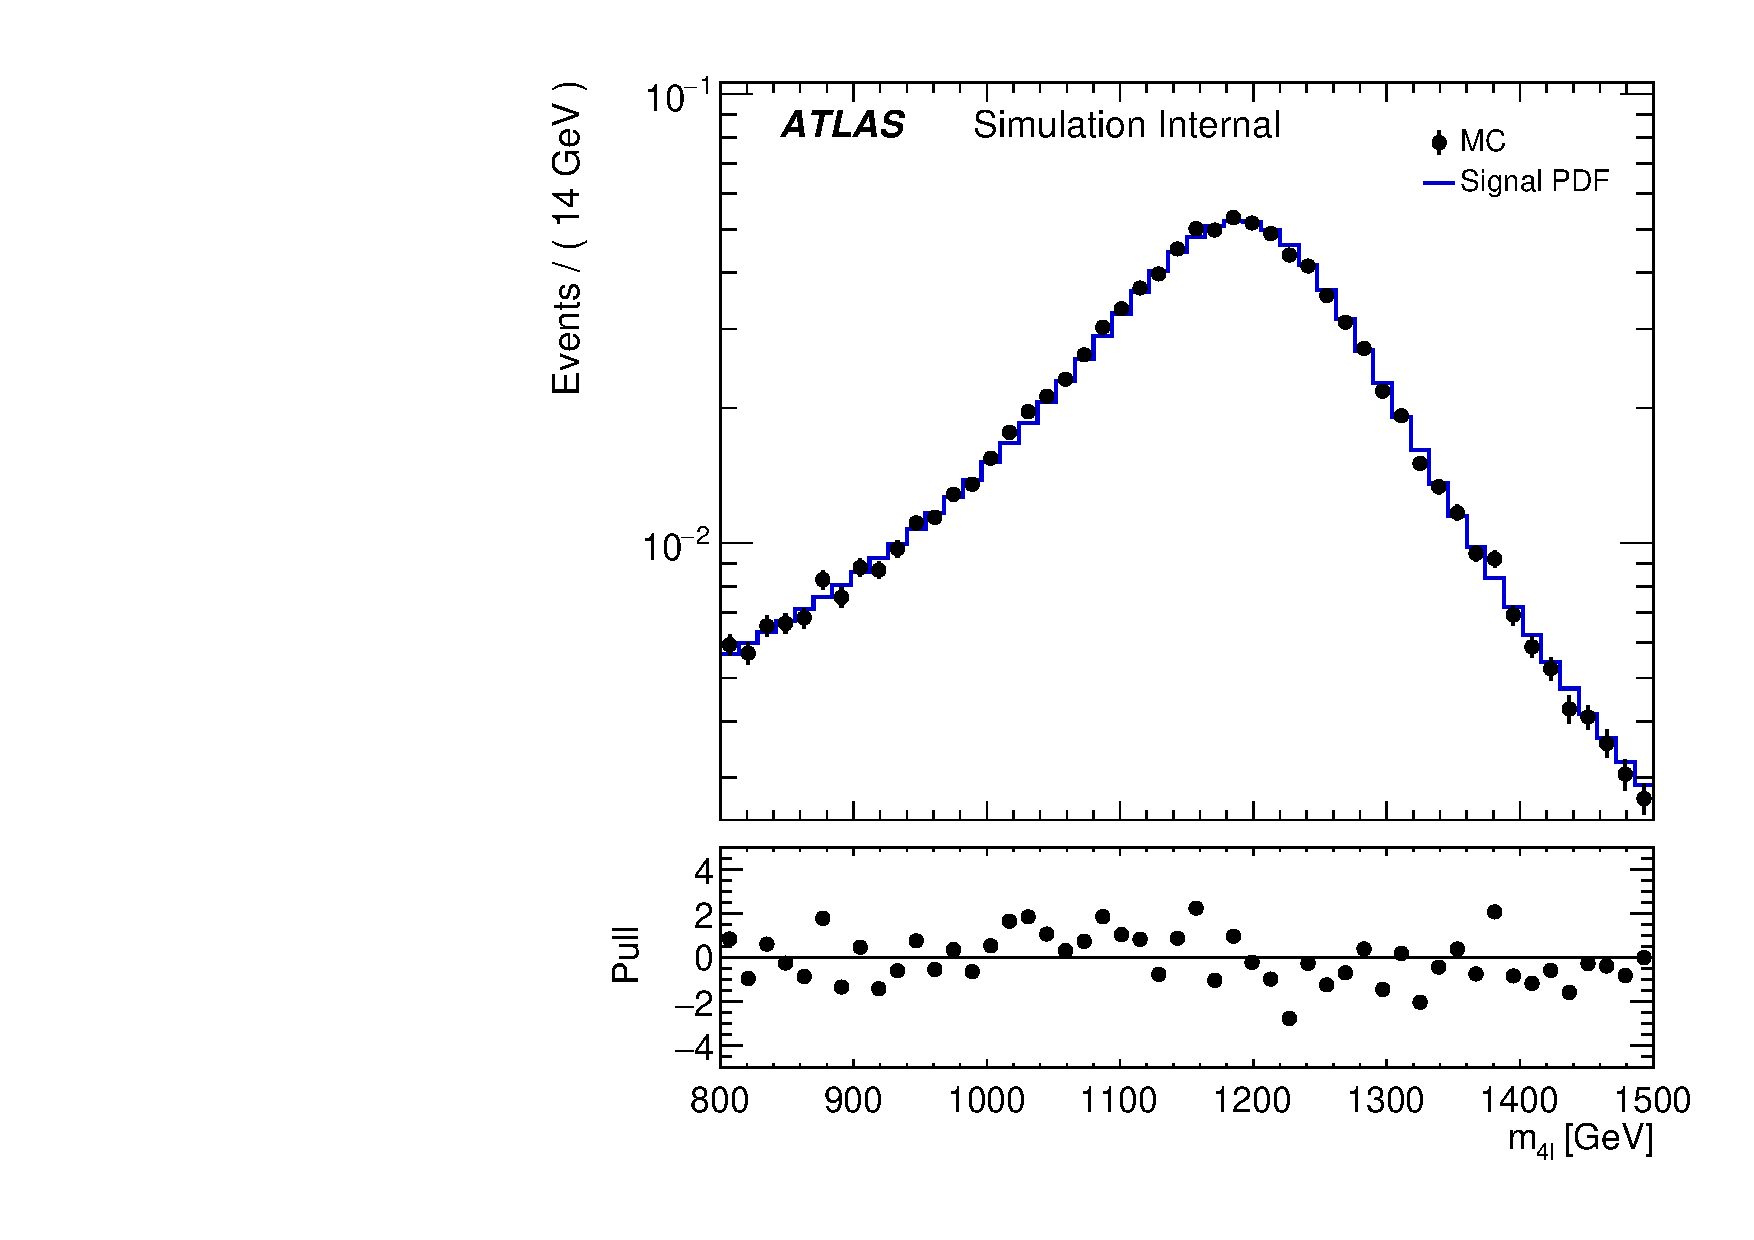
\includegraphics[width=.32\textwidth]{figures/HMHZZ/signal/LWA/cmp_1200GeV_ATLAS_Signal_ggF_ggF_2mu2e_13TeV_conv.pdf}
    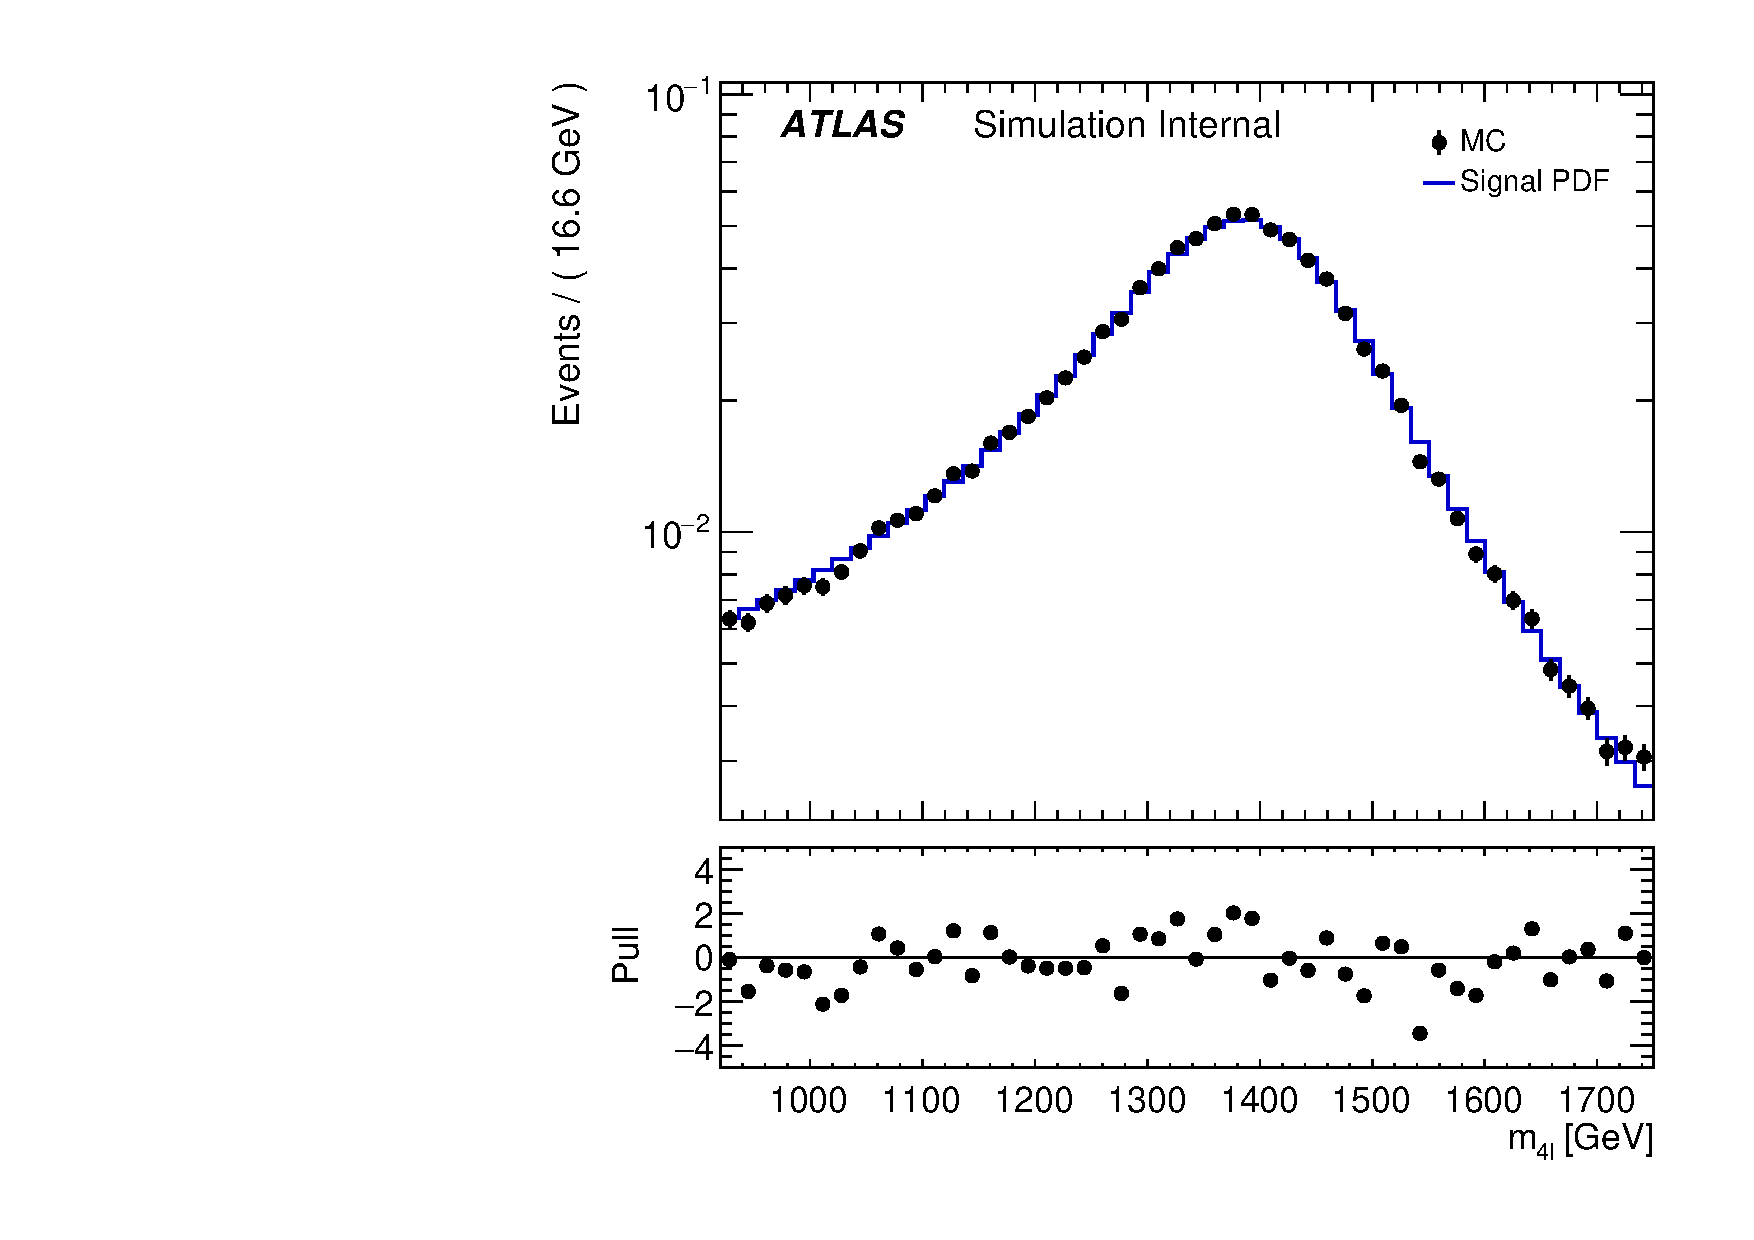
\includegraphics[width=.32\textwidth]{figures/HMHZZ/signal/LWA/cmp_1400GeV_ATLAS_Signal_ggF_ggF_2mu2e_13TeV_conv.pdf}
    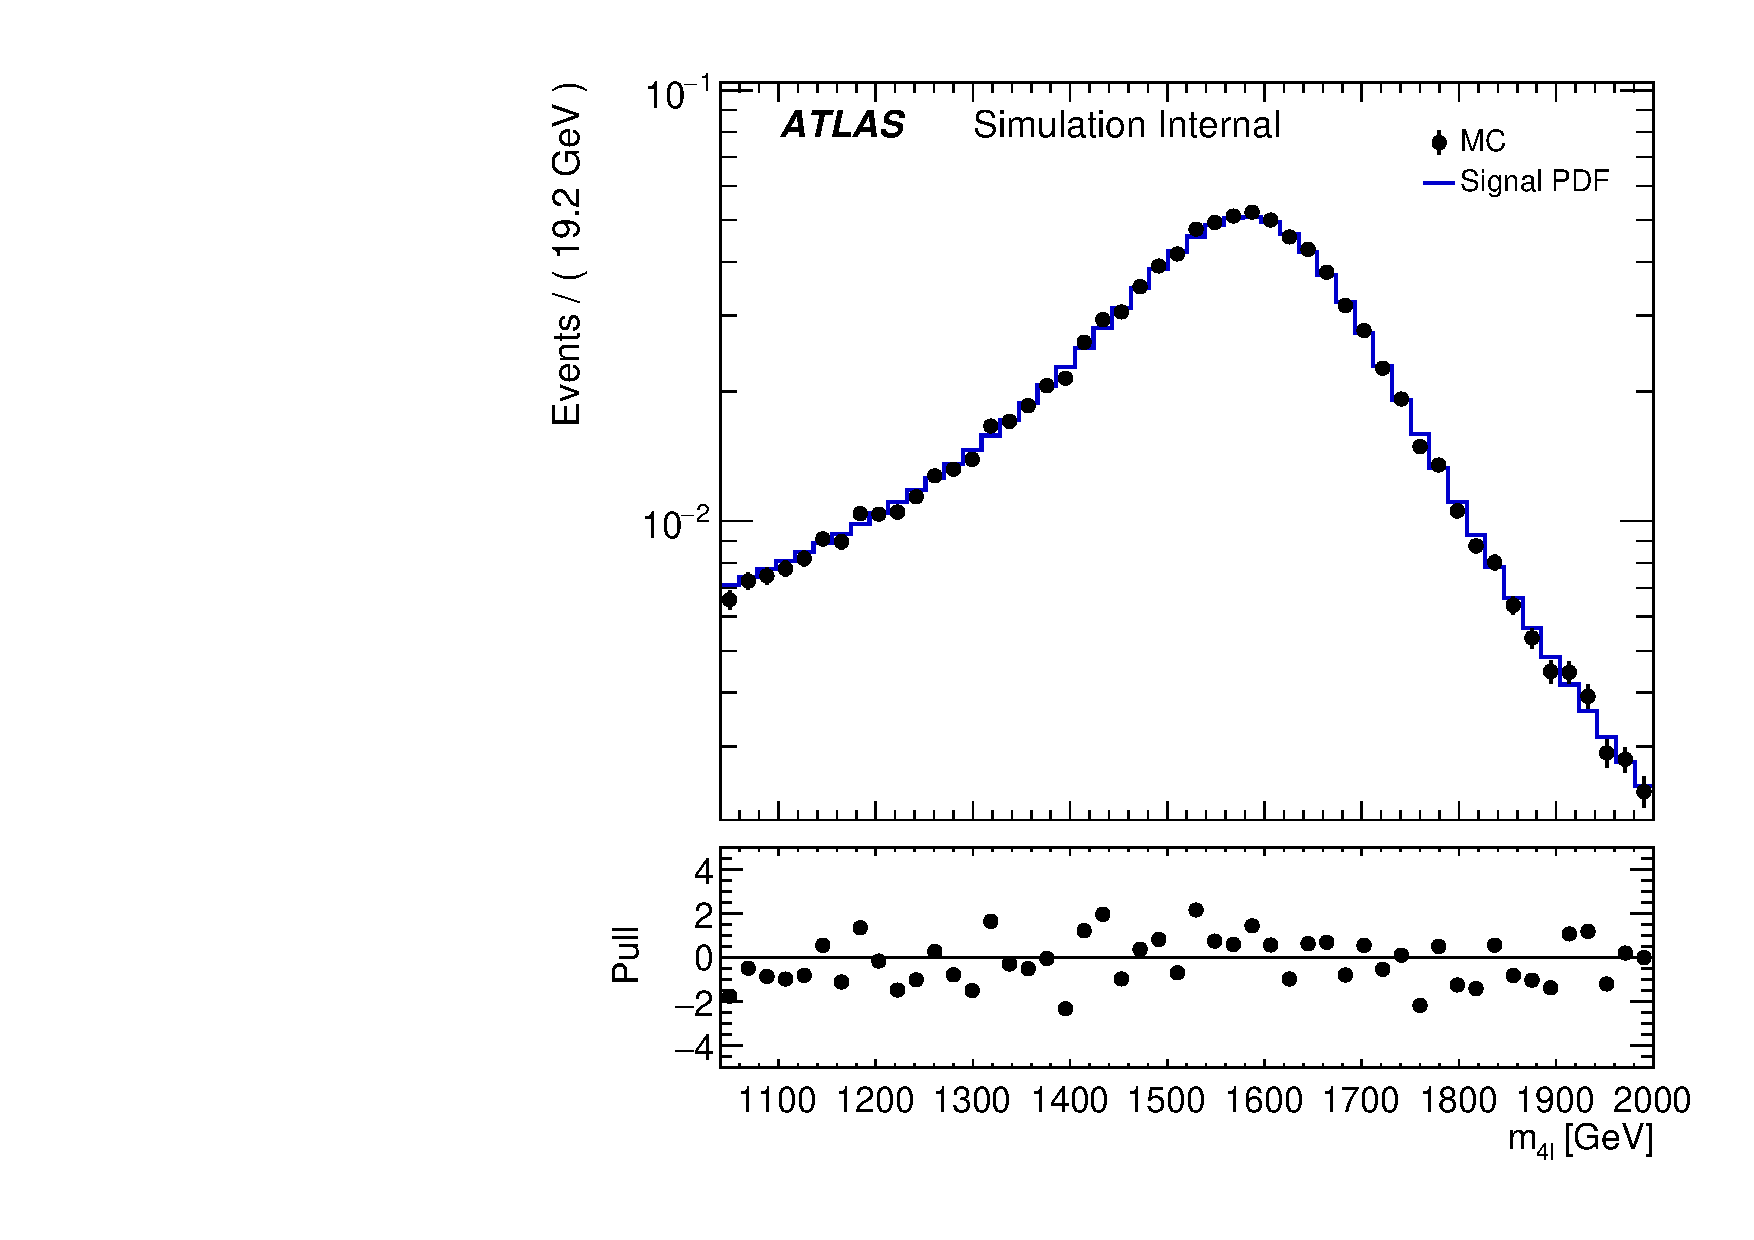
\includegraphics[width=.32\textwidth]{figures/HMHZZ/signal/LWA/cmp_1600GeV_ATLAS_Signal_ggF_ggF_2mu2e_13TeV_conv.pdf}\\
    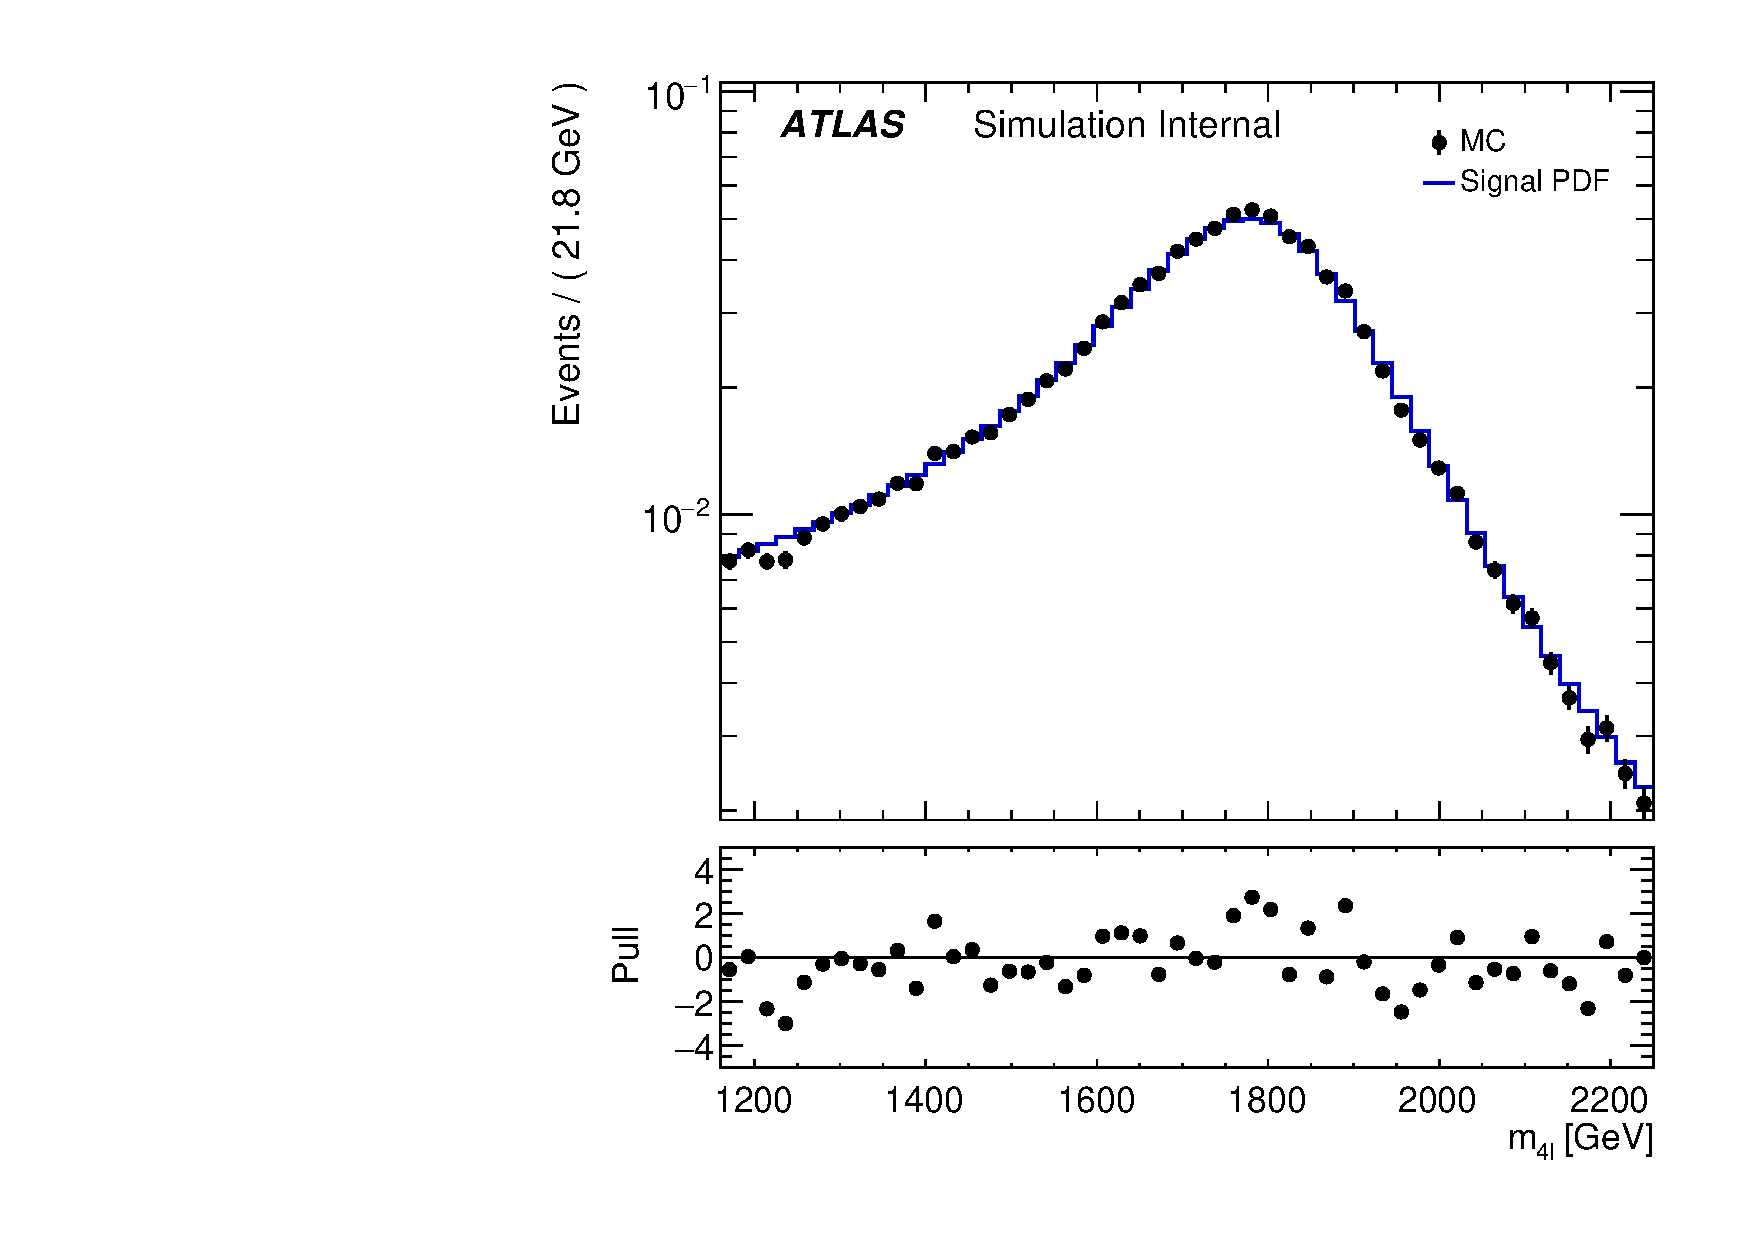
\includegraphics[width=.32\textwidth]{figures/HMHZZ/signal/LWA/cmp_1800GeV_ATLAS_Signal_ggF_ggF_2mu2e_13TeV_conv.pdf}
    \caption{Comparison between the analytical shape convoluted with detector effects and the reconstructed $m_{2\mu 2e}$ MC
    distribution for mass points ranging from 400 to 1800~$\gev$ and width equal to $15\%$ of the mass.}
    \label{fig:recoShape_2mu2e}
\end{figure}

\subsection{Modelling of interference}
\label{sec:int_model}

There are three processes sharing the same $gg$ initial state and $ZZ$ final state:
\begin{itemize}
	\item The SM \ggZZ process with an amplitude $A_{B}$
	\item The SM (light) Higgs at mass of around 125~\gev~ with an amplitude $A_{h}$
	\item The BSM heavy Higgs we are searching in this analysis with an amplitude $A_{H}$
\end{itemize}
The three processes can interfere with each other due to the same initial and final states.
The parton cross section for these processes can be written as:

\begingroup
%\small
\begin{equation} \label{eq:xsec_parton_int}
\begin{split}
    \sigma_{gg \to (X) \to ZZ} (s) &= \frac{1}{2s}  \int d \Omega \left | A_h(s,\Omega) + A_H(s,\Omega) + A_B(s,\Omega) \right |^2 \\
    &= \frac{1}{2s}  \int d \Omega  \left (  \left | A_h(s,\Omega)  \right |^2 +  \left | A_H(s,\Omega)  \right |^2 +  \left | A_B(s,\Omega)  \right |^2  \right )  + \\
    &+ \frac{1}{s}  \int d \Omega  \big( Re \left [ A_h(s,\Omega) \cdot A^*_B(s,\Omega)  \right ] \\
    &+ Re \left [ A_H(s,\Omega) \cdot A^*_B(s,\Omega)  \right ] + Re \left [ A_H(s,\Omega) \cdot A^*_h(s,\Omega)  \right ]  \big) \\
    %&+ \frac{1}{s} \mathrm{Re} \left [ \frac{1}{s-s_H}  \int d \Omega \cdot A_H^P(s,\Omega)  \cdot A_H^D(s,\Omega) \cdot A^*_B(s,\Omega)  \right ] \\
    %&+ \frac{1}{s} \int d \Omega \cdot \mathrm{Re} \left [A_H^P(s,\Omega)\cdot  \frac{1}{s-s_H}   \cdot A_H^D(s,\Omega) \cdot A_h^{P*}(s,\Omega)\cdot  \frac{1}{(s-s_h)^*}   \cdot A_h^{D*}(s,\Omega)   \right ]
\end{split}
\end{equation}
\endgroup

The first term in equation~\ref{eq:xsec_parton_int} denotes the on-shell SM Higgs contribution, which is negligible in this analysis.
The second term corresponds to the heavy Higgs contribution, whose line shape has been described in previous section.
The third term is the \ggZZ continuum process, while the forth term is the interference between SM Higgs and \ggZZ continuum.
The fifth and sixth terms are the interferences between heavy Higgs and \ggZZ continuum (H-B), and between heavy Higgs and SM Higgs (H-h) that we are interested in.
More details about the parameterization of these two interferences are described as below.

\subsubsection{Interference between heavy Higgs and \ggZZ continuum}

The parton cross section of this interference term can be expressed as:
\begin{equation}
	\sigma_{gg} (s) = \frac{1}{s} \mathrm{Re} \left [ \frac{1}{s-s_H}  \int d \Omega \cdot A_H^P(s,\Omega)  \cdot A_H^D(s,\Omega) \cdot A^*_B(s,\Omega)  \right ]
\end{equation}
By assuming that this function has a smooth behaviour, it can be replaced with complex polynomial:
\begin{equation}
    \int d \Omega \cdot A_H^P(s,\Omega)  \cdot A_H^D(s,\Omega) \cdot A^*_B(s,\Omega)  \approx  (a_0 + a_1 \cdot \sqrt{s} + \dots) + i \cdot (b_0 + b_1 \cdot \sqrt{s} + \dots)
\end{equation}

The parameters $a_i$ and $b_i$ can be extracted by fitting to the \mfl distribution from truth level MC simulation after analysis selection.
Since the signal mass and width does not enter into this function, the parameters should be independent for every tested signal hypothesis.

Same as description for equation~\ref{eq:HiggsHadronXSection}, the parton cross section can be transformed into a hadron cross section as a function of \mfl:

\begingroup
\small
\begin{equation} \label{eq:HBHadronXSection}
    \sigma_{pp} (m_{4\ell}) = \mathcal{L}_{gg} \cdot \frac{1}{m_{4\ell}} \cdot \mathrm{Re} \left [   \frac{1}{s-s_H}  \cdot  \left ( (a_0 + a_1 \cdot m_{4\ell} + \dots) + i \cdot (b_0 + b_1 \cdot m_{4\ell} + \dots) \right )\right ]
\end{equation}
\endgroup
where the propagators are shown in equation~\ref{eq:propagator}.

Figure~\ref{fig:HB_Int_2mu2e} shows the distributions of interference function obtained by simultaneous fitting to \mfl shape from truth level H-B interference simulation at different mass in 2$e$2$\mu$ channel as an example.

\begingroup
\small
\begin{figure}[!htbp]
    \centering
    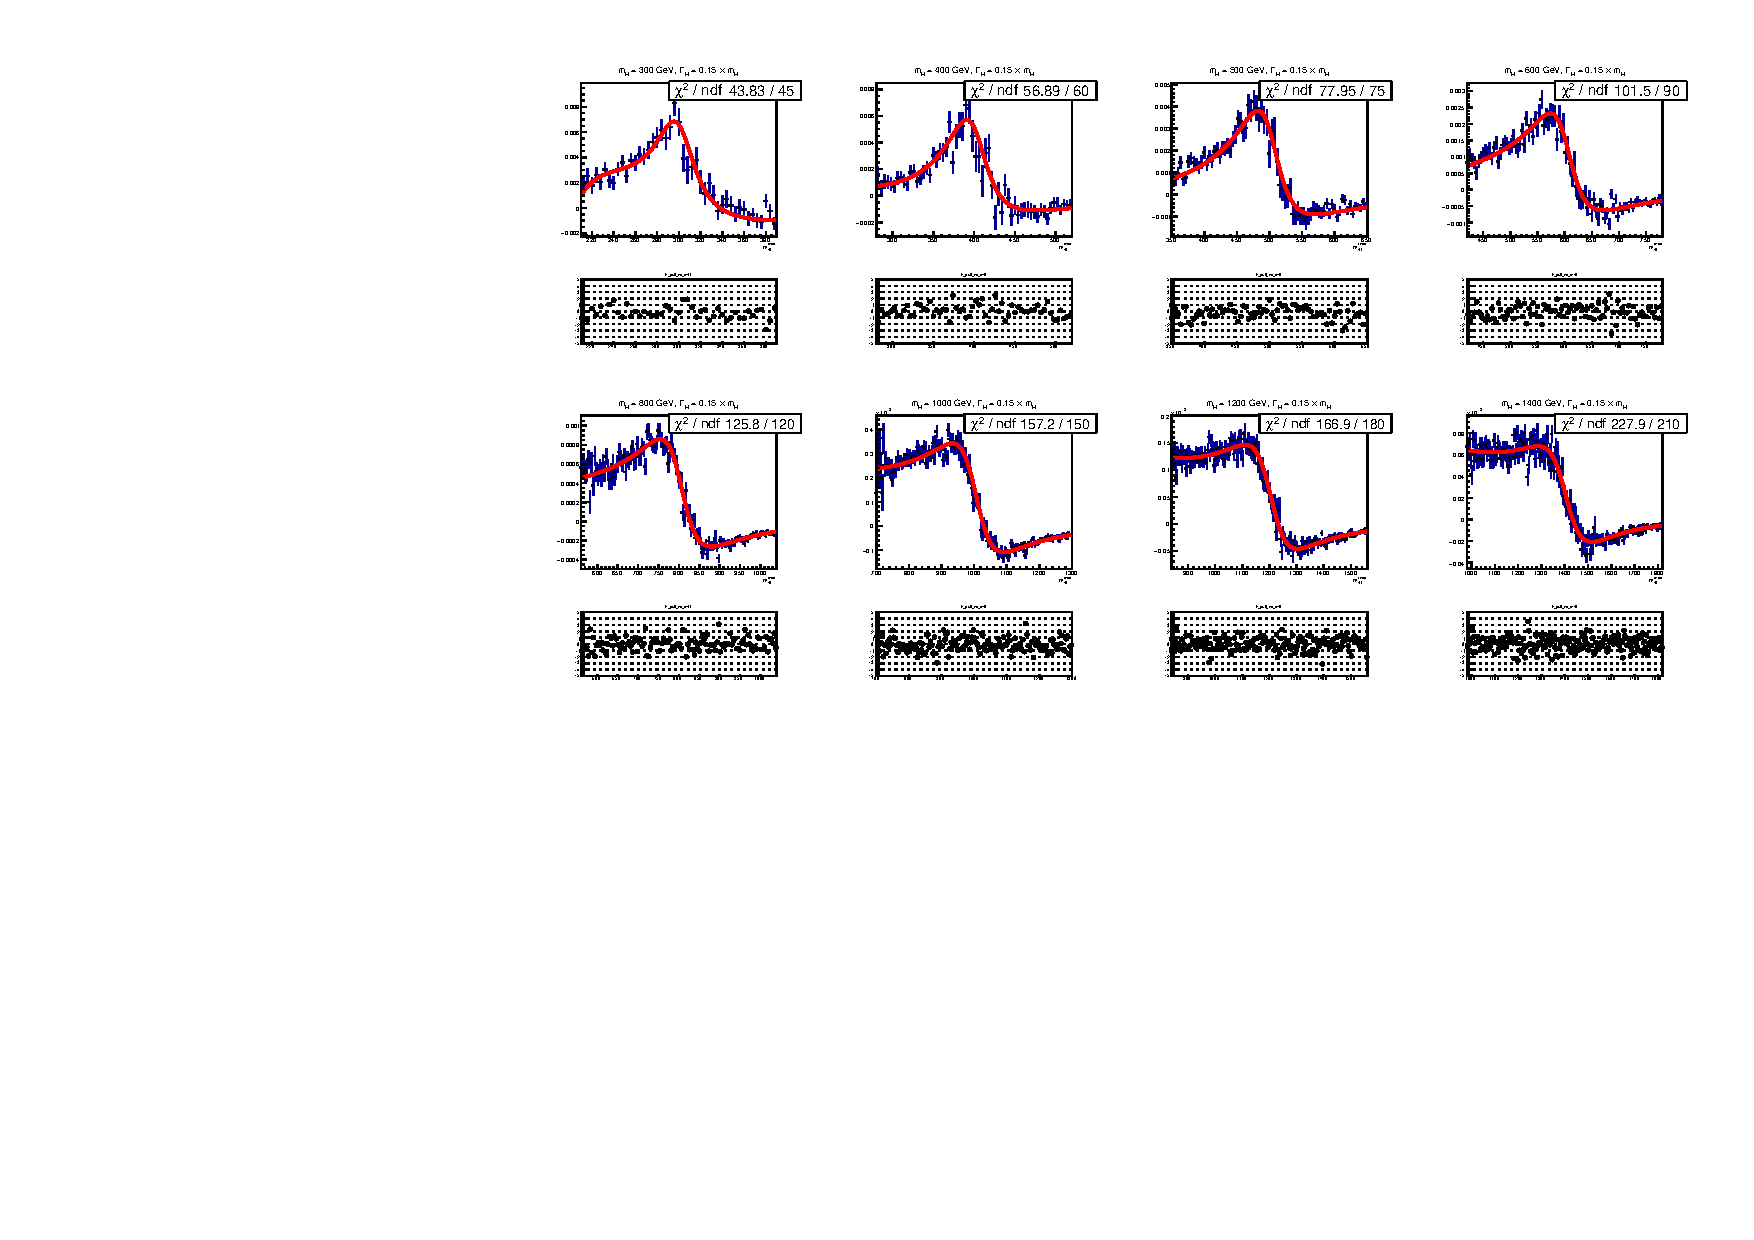
\includegraphics[width=1.\textwidth]{figures/HMHZZ/signal/Interference/HB_Int_2mu2e.pdf}
    \caption{The interference (H-B) model fitted to the truth~\mfl~MC distribution after signal region selection for $2\mu2e$~channel. \label{fig:HB_Int_2mu2e} }
\end{figure}
\endgroup

\subsubsection{Interference between heavy Higgs and SM Higgs}

The parton cross section of this interference term can be written as:
\begingroup
\small
\begin{equation}
	\sigma_{gg} (s) = \frac{1}{s} \int d \Omega \cdot \mathrm{Re} \left [A_H^P(s,\Omega)\cdot  \frac{1}{s-s_H}   \cdot A_H^D(s,\Omega) \cdot A_h^{P*}(s,\Omega)\cdot  \frac{1}{(s-s_h)^*}   \cdot A_h^{D*}(s,\Omega)   \right ]
\end{equation}
By assuming the production and decay amplitudes are the same for heavy Higgs boson and SM Higgs boson, the cross section function can be simplified to:
\begin{equation}
    \sigma_{gg} (s) = \frac{1}{s}  \int d \Omega \cdot \mathrm{Re} \left [\frac{1}{s-s_H} \cdot  \frac{1}{(s-s_h)^*} \right ] \cdot \left | A_{gg \to H}(s,\Omega) \right |^2 \left | A_{H \to ZZ}(s,\Omega) \right |^2
\end{equation}
\endgroup

Taking into account Equation~\ref{eq:PartialWidth}:

\begin{equation} \label{eq:HhInterference_2}
    \sigma_{gg} (s) = 4 \cdot \mathrm{Re} \left [\frac{1}{s-s_H} \cdot  \frac{1}{(s-s_h)^*} \right ] \cdot  \Gamma_{H \to gg} (s) \cdot \Gamma_{H \to ZZ} (s)
\end{equation}

where the propagators are described in equation~\ref{eq:propagator}, and the partial widths are described in equations~\ref{eq:WidthZZ}~and~\ref{eq:WidthGG}.

Same as previous procedure, the parton cross section can be transformed to a hadron cross section as a function of \mfl:

\begin{equation} \label{eq:HhInterference}
    \sigma_{pp} (m_{4\ell}) = 4 \cdot m_{4\ell} \cdot  \mathcal{L}_{gg}\cdot \mathrm{Re} \left [\frac{1}{s-s_H} \cdot  \frac{1}{(s-s_h)^*} \right ] \cdot  \Gamma_{H \to gg} (m_{4\ell}) \cdot \Gamma_{H \to ZZ} (m_{4\ell})
\end{equation}

%This equation is similar to the differential cross section of signal only production with the only difference in propagator.
%Since the propagator does not affect the kinematic performance of the final state, this interference process can be reproduced by reweighting the signal events with weights defined as:
%
%\begin{equation}
%    w(m_{4\ell}) = \frac{2 \cdot \mathrm{Re} \left [\frac{1}{s-s_H} \cdot  \frac{1}{(s-s_h)^*} \right ] }{\frac{1}{\left | s - s_H \right |^2}}
%\end{equation}

The modelling procedure of interference is the same as the way for large-width signal described in section~\ref{sec:signal_lwa}.
The truth line shape is measured as analytical function from equation~\ref{eq:HhInterference}, and then convolute with detector effect from NWA parameterization to get the reconstruction level shape.

For LWA signal model, these two interferences are carefully taken into account, and the integration of the pure LWA signal with the interferences is used for further studies.
Figure~\ref{fig:LWASignalModel} shows the signal model for large-width scenario at mass points of 400~\gev, 600~\gev, 800~\gev, for three different signal widths: 5\%, 10\%, 15\%, with and without interference.
Additionally, the contribution of the interference between heavy Higgs and SM Higgs (H-h) is shown together with the one between heavy Higgs and SM \ggZZ background (H-b).
One can see the interference effect on signal shape becomes less important when going to higher mass.

\begin{figure}[htbp]
    \centering
    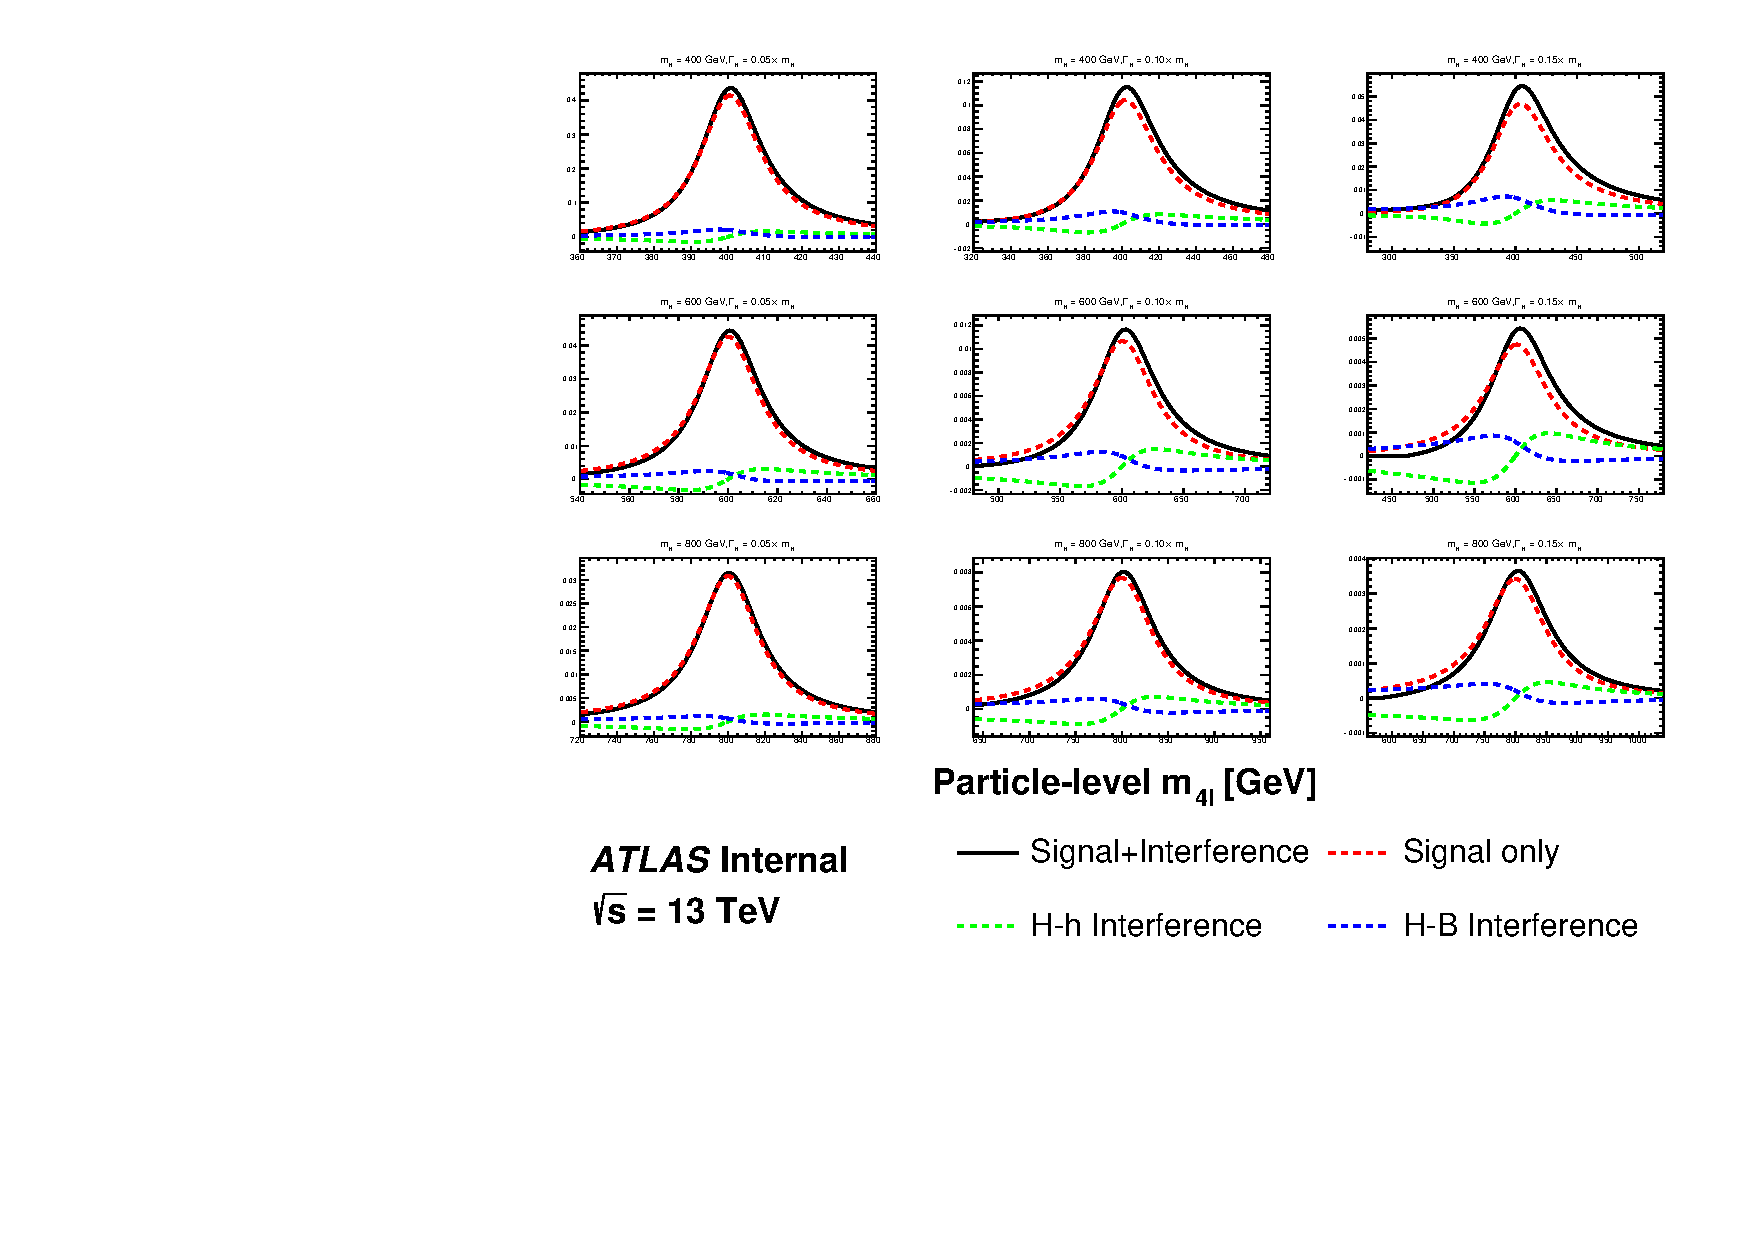
\includegraphics[width=1.0\textwidth]{figures/HMHZZ/signal/LWA/LWAModel.pdf}
    \caption{The signal modelling for the large-width scenario at \mH of 400 GeV (top), 600 GeV (middle) and 800 GeV (bottom), as well as three different signal width:  5\%  (left), 10\%  (middle) and 15\% (right). 
    The contribution of the interference between heavy Higgs and SM Higgs (H-h) is shown together with the one between heavy Higgs and SM \ggZZ background (H-b).}
    \label{fig:LWASignalModel}
\end{figure}


\subsection{Modelling of spin-2 RS Graviton signal}

The search for Randall-Sundrum (RS) graviton is performed in mass region between 600 to 2000~\gev.
The width of resonance is determined by the \kOverMpl, which, as mentioned in section~\ref{sec:hmhzz_signal_mc}, is set to be 1. 
In this configuration, the width of signal is expected to be about 6\% of its mass.

The reconstructed \mfl lineshape of graviton is also built by convolving the truth-level lineshape with a detector resolution function,
where the detector resolution effect is modelled by a Gaussian + Crystal Ball function, whose parameters are taken from the NWA signal parameterization in section~\ref{sec:signal_nwa}.
And the truth-level shape is modelled as the product of a relativistic Breit-Wigner (RBW) term, a term corresponding to the squared matrix element of the production process and a parton luminosity term $\mathcal{L}$ as given in ~\cite{Bijnens_2001}.
So the truth lineshape of \mfl is taken from:
\begin{equation*}
        \mfl^{\text{Truth}} \sim \mathcal{L}_{gg} \cdot s^2 \cdot \frac{s(1 + s)(1 + 2s + 2s^2)}{(s^2 - \mG^2)^2 + \mG^2 \Gamma^2}
\end{equation*}
The truth-level signal model is extracted by fitting to MC simulation at truth-level with the mass $\mG$ and width $\Gamma$ parameters floating at each mass points respectively.
And then the two parameters are parameterized as the function of \mH by a linear fit as shown in figure~\ref{fig:graviton_truth_param_vs_mG}.
\begin{figure}[htbp]
        \centering
        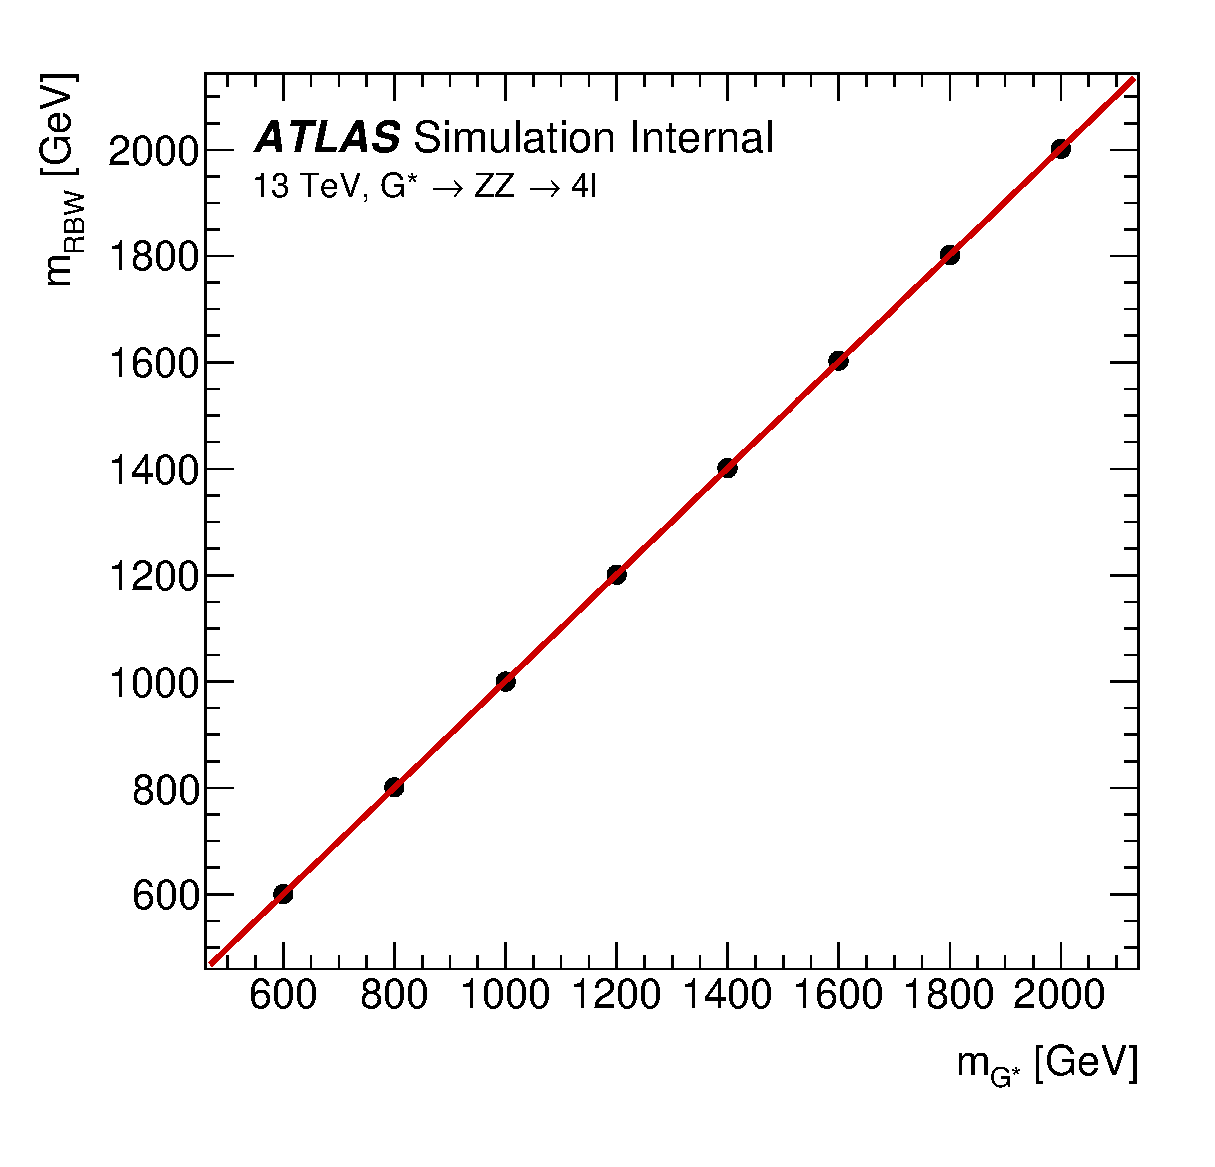
\includegraphics[width=0.4\textwidth]{figures/HMHZZ/signal/RSGraviton/graviton_param_m_RBW.eps}
        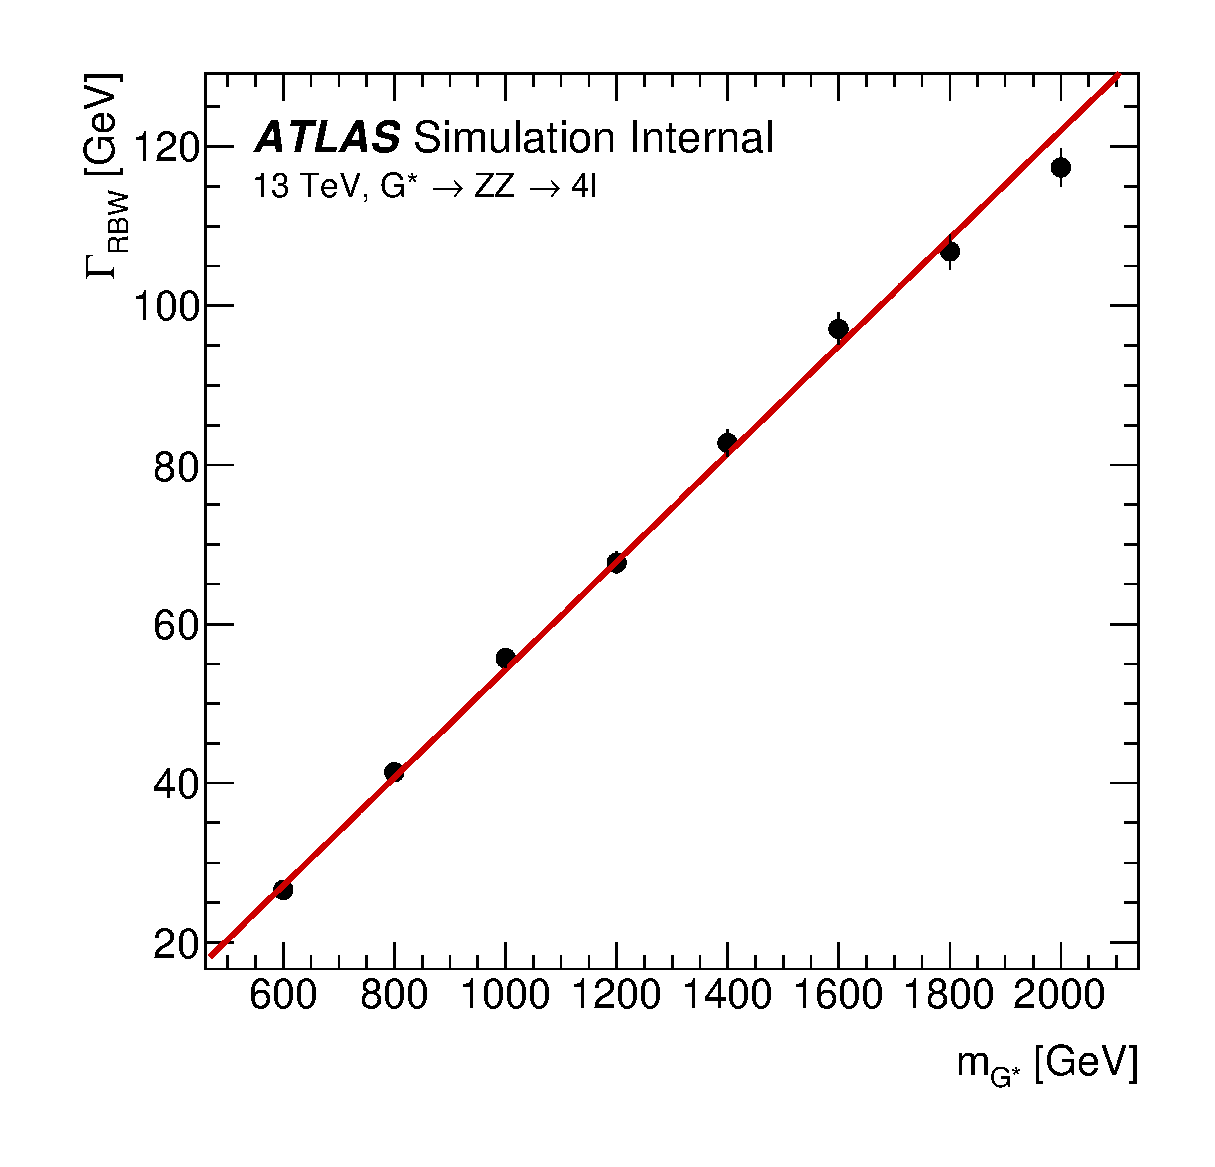
\includegraphics[width=0.4\textwidth]{figures/HMHZZ/signal/RSGraviton/graviton_param_G_RBW.eps}
        \caption{Fitted parameters of the graviton RBW, $m_{\text{RBW}}$ and $\Gamma_{\text{RBW}}$, as a function of the
        graviton resonance mass, \mG.}
        \label{fig:graviton_truth_param_vs_mG}
\end{figure}

The final signal model is obtained by convolving the truth-level lineshape with the detector resolution function.
To verify the result, figure~\ref{fig:graviton_reco_shape_2mu2e} compares the \mfl lineshape from parameterization with the one observed from reconstructed-level MC simulation in 2$e$2$\mu$ channel at masses of 600~\gev, 1600~\gev~and 2000~\gev~as examples.

\begin{figure}[htbp]
    \centering
    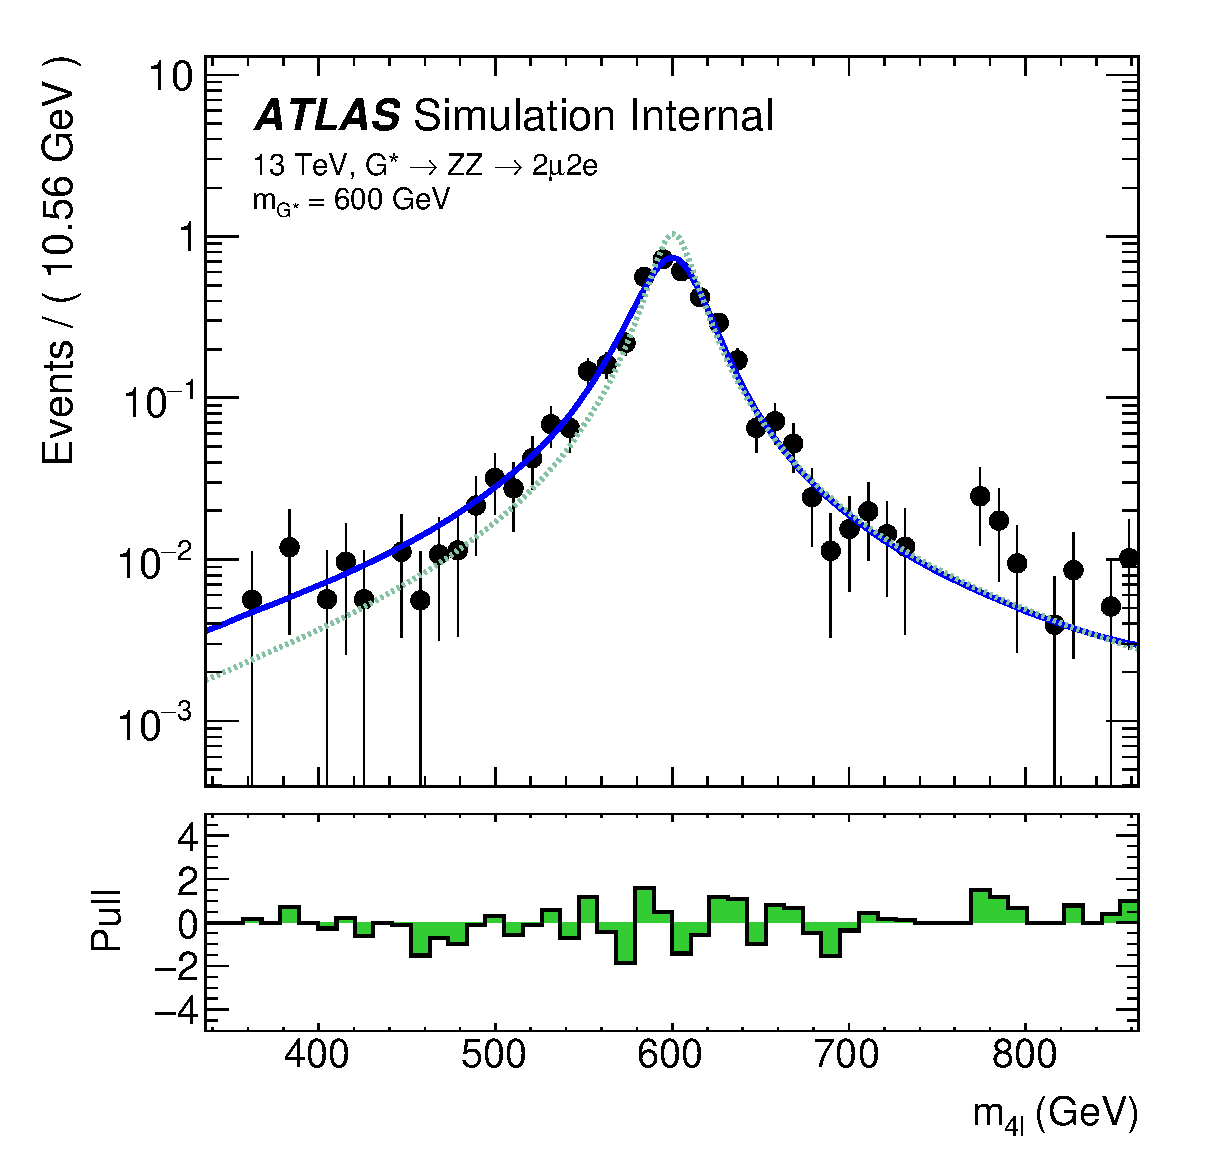
\includegraphics[width=0.32\textwidth]{figures/HMHZZ/signal/RSGraviton/graviton_reco_shape_m4l_constrained_HM_600GeV_2mu2e.eps}
    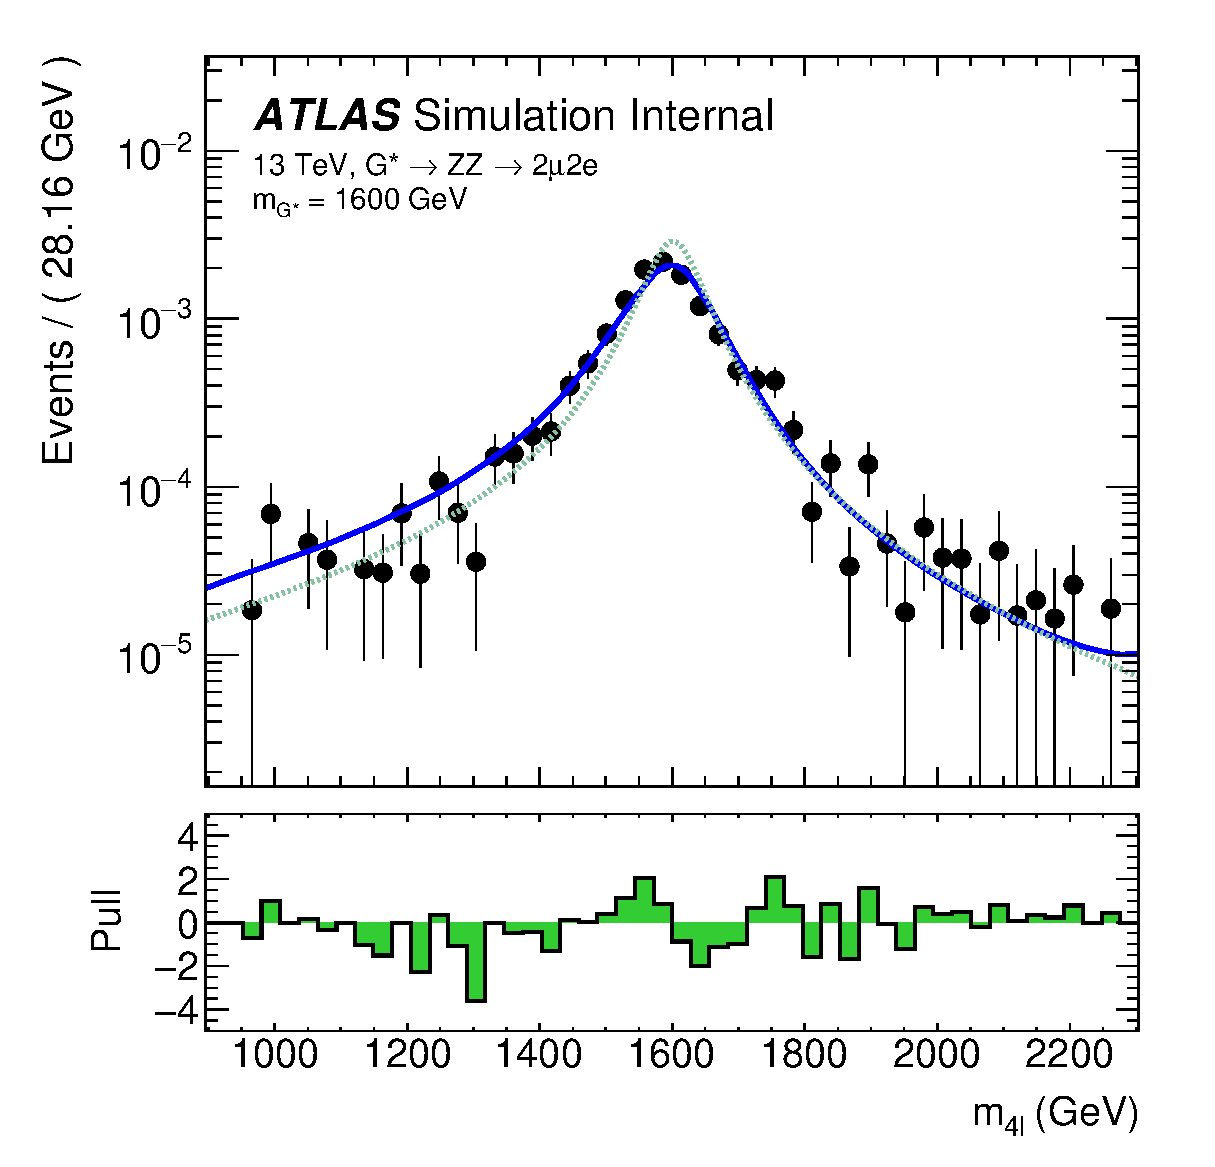
\includegraphics[width=0.32\textwidth]{figures/HMHZZ/signal/RSGraviton/graviton_reco_shape_m4l_constrained_HM_1600GeV_2mu2e.eps}
    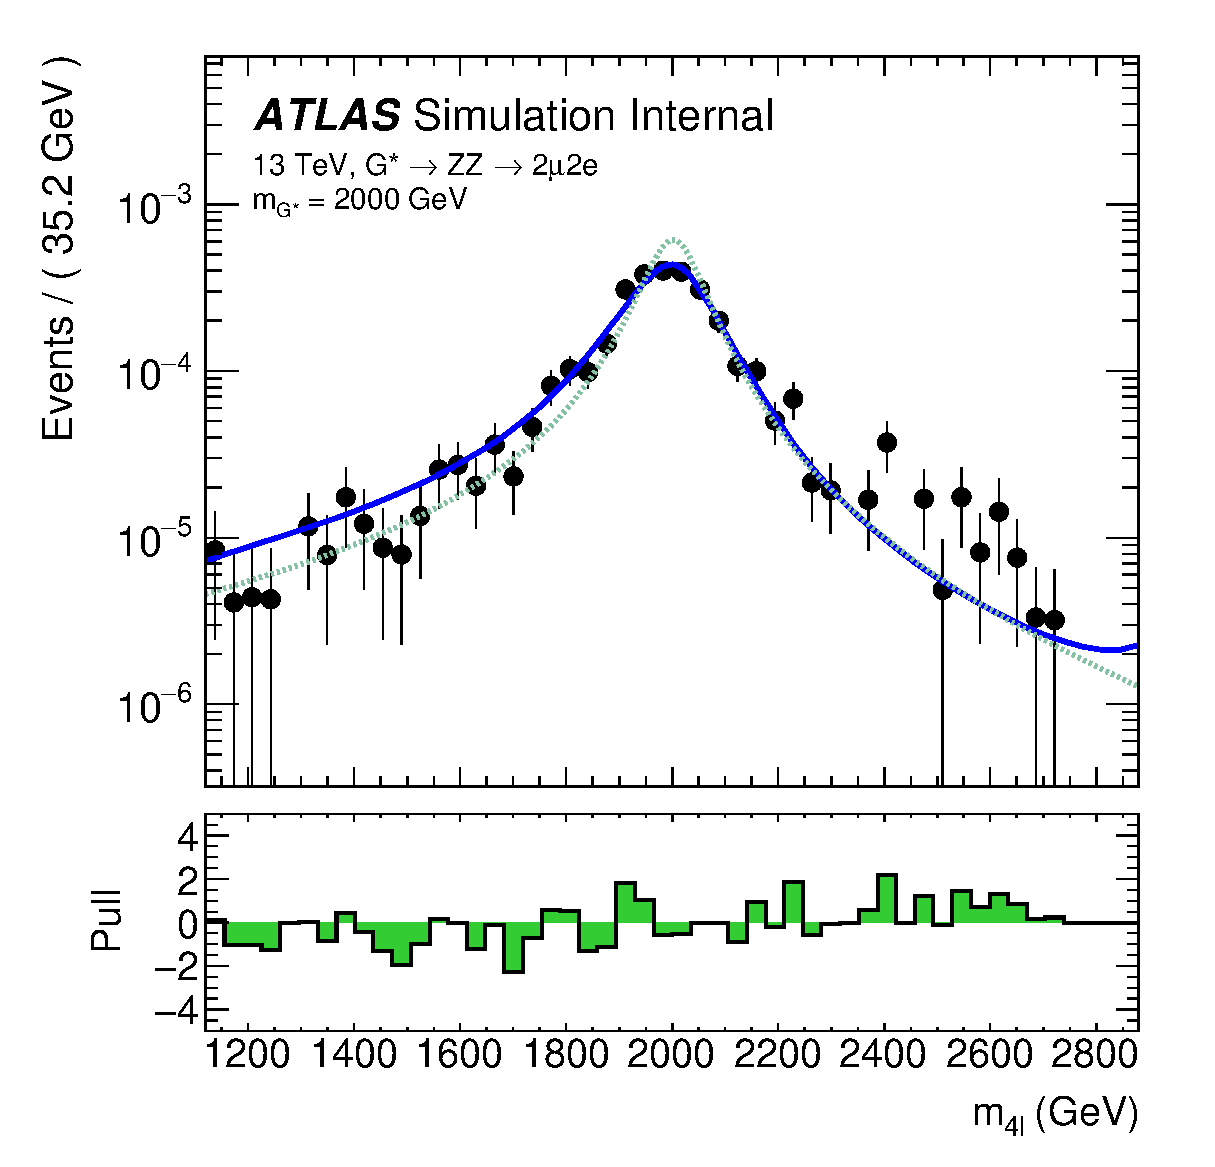
\includegraphics[width=0.32\textwidth]{figures/HMHZZ/signal/RSGraviton/graviton_reco_shape_m4l_constrained_HM_2000GeV_2mu2e.eps}
    \caption{Reconstructed \mfl distributions in the $2\mu 2e$ channel with the final signal
        model superimposed for each RS graviton signal sample at masses of 600~$\gev$, 1600~$\gev$ and 2000~$\gev$. The lower panel in each plot shows
        the pull distribution. The dashed green lines show the truth-level graviton signal models for reference.}
    \label{fig:graviton_reco_shape_2mu2e}
\end{figure}
